\documentclass[11pt]{report} % Schriftgrösse 11
\usepackage{graphicx} % Required for inserting images
\usepackage[english, german]{babel}
\usepackage{lipsum}
\usepackage{csquotes}
%\usepackage[PetersLenny]{fncychap}
\usepackage{amsmath}
\usepackage{array}
\usepackage{float}
\usepackage{amssymb}
\usepackage[many]{tcolorbox}
\tcbuselibrary{theorems}
\usepackage[framemethod=TikZ]{mdframed} % noteboxes, boxes, etc.
\usepackage{tocloft}
\usepackage{svg}
\usepackage{pgfplots}
\pgfplotsset{width=9cm,compat=1.18}


\usepackage[%
    left=3.5cm,%
    right=3cm,%
    top=2.5cm,%
    bottom=3cm,%
]{geometry}%

\usepackage[style=apa,sorting=anyt]{biblatex}
\addbibresource{bibli.bib}
% Überschreibe das Format für die Überschrift des Literaturverzeichnisses
\defbibheading{myheading}[Literaturverzeichnis]{%
  \section{#1}%
  \markboth{#1}{#1}%
}

\renewcommand{\baselinestretch}{1.5} % Zeilenabstand

% DEFINITION DER COMMANDS FÜR PARTIELLE ABLEITUNGEN UND N-TER PARTIELLER ABLEITUNGEN
\newcommand\pd[2]{\displaystyle\frac{\partial #1}{\partial #2}}
\newcommand\nthpd[3]{\displaystyle\frac{\partial^#3 #1}{\partial #2^#3}}

\newtcbtheorem[auto counter]{Theorem}{Theorem}%
{colback=red!5,colframe=red!35!black,fonttitle=\bfseries, breakable}{th}
\newtcbtheorem[auto counter]{Beispiel}{Beispiel}%
{colback=blue!5,colframe=blue!35!black,fonttitle=\bfseries, breakable}{ex}
\newtcbtheorem[auto counter]{Definition}{Definition}%
{colback=black!5,colframe=black!35!black,fonttitle=\bfseries, breakable}{def}
\newtcbtheorem[auto counter]{Beweis}{Beweis}%
{colback=green!5,colframe=green!35!black,fonttitle=\bfseries, breakable}{proof}

\usepackage{listings}
\usepackage{color}

\definecolor{dkgreen}{rgb}{0,0.6,0}
\definecolor{gray}{rgb}{0.5,0.5,0.5}
\definecolor{mauve}{rgb}{0.58,0,0.82}

\lstset{frame=tb,
  language=Python,
  aboveskip=3mm,
  belowskip=3mm,
  showstringspaces=false,
  columns=flexible,
  basicstyle={\normalsize\ttfamily},
  numbers=none,
  numberstyle=\tiny\color{gray},
  keywordstyle=\color{blue},
  commentstyle=\color{dkgreen},
  stringstyle=\color{mauve},
  breaklines=true,
  breakatwhitespace=true,
  tabsize=3
}

\title{\textbf{Reich werden mit Mathematik}\\Methoden zur Optionspreisberechnung und Entwicklung eines Pricing-Tools}
\author{Nils Blunier}
\date{\today}

\begin{document}

\begin{titlepage}
    \vspace*{\fill}
    \begin{center}
        \vspace{1cm}
        \Huge \textbf{Reich werden mit Mathematik}\\Methoden zur Optionspreisberechnung und Entwicklung eines Pricing-Tools \\
        \vspace{1cm}
        \Large Wettbewerbsarbeit für Schweizer Jugend forscht\\Nils Blunier\\Neue Kantonsschule Aarau\\ \today{}
    \end{center}
    \vspace*{\fill}
    \begin{flushright}
        \Large Experte von Schweizer Jugend forscht: Matthias Grützner\\Lehrperson an der Neuen Kantonsschule Aarau: Dr. Maik Berchtold
    \end{flushright}
\end{titlepage}

\selectlanguage{english}
\begin{abstract}
Das Ziel der vorliegenden Arbeit ist, die Binomialmodellformeln, die Black-Scholes-Formeln und die rekursive Berechnungsmethode für amerikanische Optionspreise selber zu verstehen und verständlich zu erklären. Es wird gezeigt, wie mithilfe von Monte-Carlo-Simulationen europäische Optionspreise berechnet werden können. Zudem wird ein Pricing-Tool programmiert, mit dem man den Preis einer gewünschten Option berechnen kann. Es wird zudem der Einfluss von verschiedenen Parametern auf den europäischen und amerikanischen Optionspreis untersucht. Ausserdem werden Long- und Short-Butterfly-Spreads besprochen und gezeigt, wie man den Preis von Optionen mit einer beliebigen Payoff-Funktion berechnet. Es wird gezeigt, dass der Call-Optionspreis positiv vom Aktienpreis, dem risikolosen Zinssatz, der Volatilität und der Laufzeit und negativ vom Ausübungspreis beeinflusst wird. Der Put-Optionspreis wird positiv vom Ausübungspreis und der Volatilität und negativ vom Aktienpreis und dem risikolosen Zinssatz beeinflusst. Die Annahmen, die getroffen werden, um die Pricing-Formeln herzuleiten, werden kritisiert, da sie viele reale Begebenheiten missachten und so ein verfälschtes Resultat liefern. Zudem würde sich für niedrige Modellschrittzahlen das Trinomialmodell besser als das Binomialmodell zur Optionspreisberechnung eignen. Die Benutzeroberfläche des Pricing-Tools könnte man gestalterisch noch weiter ausbauen und die programmiertechnische Berechnung von amerikanischen Optionspreisen möglicherweise effizienter umsetzen.

\end{abstract}
\selectlanguage{german}

\chapter*{Vorwort}
Schon seit längerer Zeit interessiere ich mich sehr fest für Mathematik und die Finanzwelt. Deshalb war bereits klar, dass ich meine Maturaarbeit zu einem finanzmathematischen Thema schreiben werde. Auf Vorschlag von Herrn Berchtold entschied ich mich schlussendlich für die Berechnung von Optionspreisen. Diese Arbeit hat mir unglaublich viel Spass gemacht, ich bin sehr dankbar für die Möglichkeit, mich so intensiv mit einem Thema meiner Wahl zu beschäftigen. Nach rund 170 Stunden Arbeitszeit bin ich äusserst zufrieden mit dem Endprodukt und zugegebenermassen auch ein wenig stolz auf mich selber. Nichtsdestotrotz hätte ich diese Arbeit niemals im totalen Alleingang bewältigen können. Ich bedanke mich deshalb herzlichst bei meiner Betreuungsperson Dr. Maik Berchtold für den Themenvorschlag, die allzeitige, sehr hilfreiche fachliche Unterstützung und die konstruktive Zusammenarbeit. Ich danke Matthias Grützner von der ETH Zürich, dem Experten von Schweizer Jugend forscht, für die anregenden Besprechungen und die hilfreichen Ratschläge. Zudem bedanke ich mich bei Steven Roman, der das Buch \textit{Introduction to the Mathematics of Finance: Arbitrage and Option Pricing} geschrieben hat, welches so verständlich formuliert ist, dass sogar ich als Kantonsschüler es verstehen konnte. Ich möchte mich zuletzt noch bei meiner Freundin bedanken, die während des anstrengenden Arbeitsprozesses immer für mich da war und mentale Unterstützung bot.
\\\\
\includesvg[width=5cm]{images/signature-better.svg}\\Nils Blunier
\newpage
\tableofcontents
\newpage

\chapter{Einleitung}
Eine Option ist das Recht, etwas zu bzw. bis zu einem bestimmten Zeitpunkt zu kaufen bzw. verkaufen zu einem im Voraus abgemachten Preis. Mit Optionen wurde bereits in der Antike gehandelt. So habe der griechische Philosoph Thales im Winter bereits geahnt, dass die Olivenernte im Sommer gut werden sollte und hat viele Olivenölpressen zu einem guten Preis reserviert. Als im Sommer die Olivenernte tatsächlich ausserordentlich ertragreich war, konnte Thales die Ölpressen für mehr Geld vermieten, als er im Winter bezahlt hatte (Thales, \cite{wikithales2024}). Wie viel Thales damals für das Recht, die Ölpressen bereits im Voraus zu reservieren, bezahlt hat, weiss man heute nicht. Die Frage, wie hoch ein Optionspreis sein sollte, beschäftigt dennoch bis heute Investoren, Banken, Mathematiker und sonstig Interessierte. \textcite{Black1973} und \textcite{Merton1973} lieferten praktisch zeitgleich eine Berechnungsmöglichkeit, welche heute als Black-Scholes-Formeln bzw. Black-Scholes-Merton-Formeln bekannt sind. Merton und Scholes erhielten 1997 den Wirtschaftsnobelpreis für ihre Leistung, Black war zu diesem Zeitpunkt bereits verstorben. 1979 veröffentlichten \textcite{Cox1979} mit den Binomialmodellformeln eine Berechnungmethode für Optionspreise, welche mithilfe von einfacherer Mathematik hergeleitet werden kann als die Black-Scholes-Formeln.\\Die vorliegende Arbeit beschäftigt sich mit der mathematischen Herleitung der Black-Scholes-Formeln und der Binomialmodellformeln. Zusätzlich wird die rekursive Berechnung von amerikanischen Optionspreisen behandelt. Die theoretischen Überlegungen und die Notation stammen aus dem Buch \textit{Introduction to the Mathematics of Finance: Arbitrage and Option Pricing} von Steven Roman. Da praktisch alle Theorie in den Kapiteln 3, 4 und 5 aus dem Buch von \textcite{Roman2012-sk} stammt, wird in diesen Kapiteln -- gemäss Absprache mit Herrn Berchtold -- nicht immer noch zitiert. Zusätzlich zu der theoretischen Herleitung der Pricing-Methoden wird der Einfluss von unterschiedlichen Parametern auf den Optionspreis untersucht, es wird die Preisberechnung von Optionen mit anderen Payoff-Strukturen, namentlich Butterfly-Spreads und Optionen mit frei wählbaren Payoff-Funktionen, besprochen und die Programmierung eines Pricing-Tools mithilfe von Python dokumentiert. Der Programmcode ist sowohl im Anhang als auch online auf \texttt{https://github.com/nlsblnr/MA} zu finden. In der vorliegenden Arbeit wird grundsätzlich das generische Maskulinum verwendet.\\Das Ziel der Arbeit war erstens, dass ich die Theorie gut verstehe und an Beispielen anwenden kann. Das zweite Ziel war, dass ein Mitschüler die mathematische Herleitung ohne fremde Hilfe nachvollziehen kann und drittens anschliessend mithilfe des von mir programmierten Pricing-Tools gewünschte Optionspreise berechnen kann. Die Kapitel zum Einfluss von gewissen Parametern auf den Optionspreis und der Betrachtung von Optionen mit anderen Payoff-Strukturen geht über den in der Projektvereinbarung festgelegten Rahmen hinaus und soll interessierten Lesern noch mehr Inhalt bieten und das Verständnis des Themas erweitern.

\chapter{Grundlagen}
\section{Was sind Optionen?}
\begin{Definition}{Option}{def-option}
    Optionen sind Verträge zwischen Käufern und Verkäufern. Der Käufer bezahlt eine bestimmte Menge Geld -- den \textit{Optionspreis} -- für das Recht,
    \begin{itemize}
        \item ein Wertpapier (z. B. eine Aktie)
        \item zu einem vereinbarten Zeitpunkt (\textit{europäische} Option) oder innerhalb eines vereinbarten Zeitraums (\textit{amerikanische} Option)
        \item in einer vereinbarten Menge (z. B. 50 Stück)\footnote{Grundsätzlich wird in dieser Arbeit aber angenommen, dass eine Option für genau ein Wertpapier gilt.}
        \item zu einem festgelegten Preis (\textit{Ausübungspreis}, engl. \textit{exercise price})
        \item zu kaufen (\textit{Call}-Option) oder zu verkaufen (\textit{Put}-Option).
    \end{itemize}
\end{Definition}

Der Käufer kauft mit der Option also einfach das Recht, z. B. eine Aktie zu kaufen. Er muss dieses Recht aber nicht ausüben und darf die Option auch einfach verfallen lassen. Wenn der Käufer eine Call-Option kauft, hofft er darauf, dass der Marktwert der Aktie über den Ausübungspreis steigt. Ist das der Fall, übt er die Option aus und darf die Aktie für weniger Geld kaufen, als sie eigentlich kosten würde. Der Verkäufer der Option hingegen hofft darauf, dass der Aktienpreis unter den Ausübungspreis sinken wird. Ist dies der Fall, wird der Käufer die Option nicht ausüben und der Verkäufer kann einfach den Optionspreis behalten, den der Käufer zu Beginn bezahlt hat.\\
Bei einer Put-Option funktioniert es umgekehrt: Der Käufer hofft, dass die Option unter den Ausübungspreis sinken wird und er die Aktie für mehr Geld verkaufen kann, als sie eigentlich kosten würde. Der Verkäufer hingegen setzt darauf, dass die Aktie über dem Ausübungspreis bleibt und er wieder einfach den Optionspreis einstreichen kann (\cite{Becker2018}, S. 303--307).


\section{Anwendungen von Optionen}
\subsection{Hedging}
Investoren benutzen sogenannte Hedging-Methoden, um ihr Portfolio vor starken und schnellen Verlusten zu schützen. So können z. B. Put-Optionen auch als Hedging-Instrumente verwendet werden. Ein Investor kauft also Put-Optionen auf ein Wertpapier, das er besitzt. Den Ausübungspreis setzt er so, dass im Falle, dass er die Option ausübt, kein allzu grosser Verlust entsteht. Wenn das Wertpapier, für das der Investor die Put-Optionen gekauft hat, plötzlich massiv an Wert verliert und unter den vereinbarten Ausübungspreis sinkt, kann der Investor die Option ausüben und das Wertpapier für mehr Geld verkaufen, als es eigentlich wert wäre. Er verringert so den Verlust, den er mit dem Wertpapier macht (\cite{Yates_2022}).
\begin{Beispiel}{}{}
    Ein Investor besitzt am 6. April 2024 100 Apple-Aktien. Momentan ist jede Aktie \$170\footnote{https://finance.yahoo.com/quote/AAPL/ (Abgerufen am 6. April 2024)} wert. Er kauft nun Put-Optionen mit Ausübungsdatum 3. Mai 2024 und Ausübungspreis \$170 für je \$4.65\footnote{https://finance.yahoo.com/quote/AAPL/options?date=1714694400 (Abgerufen am 6. April 2024)}. Er bezahlt also insgesamt $100\cdot\$4.65=\$465$. Wenn bis am 3. Mai der Kurs der Aktie auf \$150 fällt, übt der Investor seine Optionen aus und darf die Aktien für den Ausübungspreis \$170 verkaufen. Er verliert nur das Geld, das er für die Optionen bezahlt hat, also \$465. Hätte er die Optionen nicht besessen, hätte er $100\cdot(\$170-\$150)=\$2000$ Verlust gemacht. So kann man sich mithilfe von Put-Optionen gegen zu grosse Verluste absichern.
\end{Beispiel}

\subsection{Spekulation}
Mit Optionen kann zudem spekuliert werden. Das heisst, dass man auf eine bestimmte Kursentwicklung hofft und Optionen kauft, die sich lohnen, wenn die Anlage tatsächlich die erhoffte Kursentwicklung durchmacht (\cite{Yates_2022}).
\begin{Beispiel}{}{}
    Eine Aktie kostet momentan \$100. Eine Investorin geht davon aus, dass die Aktie in einem Jahr sehr viel mehr wert sein wird. Sie kauft 50 Call-Optionen mit Ausübungspreis \$110 für je \$20. Sie bezahlt also $50\cdot\$20=\$1000$. Ein Jahr später ist der Wert der Aktie auf \$150 gestiegen. Als Optionsbesitzerin darf sie jetzt 50 Aktien zum Preis von insgesamt $50\cdot\$110=\$5500$ kaufen. Da die Aktie aber eigentlich auf dem Markt für \$150 verkauft wird, kann sie ihre 50 Aktien für insgesamt $50\cdot\$150=\$7500$ verkaufen. Sie hat insgesamt also einen Gewinn von $\$7500-\$5500-\$1000=\$1000$ gemacht.
\end{Beispiel}
\begin{Beispiel}{}{}
    Eine Aktie kostet momentan \$100. Ein Investor geht davon aus, dass der Aktienpreis im nächsten Jahr sehr stark sinken wird. Er kauft 50 Put-Optionen mit Ausübungspreis \$90 für je \$20. Er bezahlt also $50\cdot\$20=\$1000$. Ein Jahr später ist der Wert der Aktie auf \$50 gesunken. Der Investor kauft nun 50 Aktien für insgesamt $50\cdot\$50=\$2500$. Als Optionsbesitzer darf er diese 50 Aktien für den Ausübungspreis von \$90 verkaufen, womit er $50\cdot\$90=\$4500$ einnimmt. Insgesamt hat der Investor also einen Gewinn von $\$4500-\$2500-\$1000=\$1000$ gemacht.
\end{Beispiel}

\section{Optionspreis}
Wie oben erwähnt, bezahlt der Käufer dem Verkäufer für die Option den Optionspreis. Doch wie hoch ist dieser?\\
Man betrachte eine Option, die sofort ausgeübt werden muss, weil man am Ende der Laufzeit der Option angekommen ist. Eine Call-Option ist in diesem Fall wertlos, wenn der Aktienpreis $S_T$ unter dem Ausübungspreis $K$ liegt, weil man die Aktie ja einfach billiger auf dem normalen Markt kaufen könnte, statt die Option auszuüben. Liegt der Aktienpreis hingegen über dem Ausübungspreis, lohnt sich die Option und der Wert der Option ist gleich dem Unterschied zwischen dem Aktienpreis und dem Ausübungspreis. Mathematisch ausgedrückt ist der Preis der Call-Option am Tag der Ausübung (europäisch) bzw. am Ende der Laufzeit (amerikanisch)
$$C_T=\max\{0, S_T-K\}=(S_T-K)^+=
\begin{cases}
  S_T-K & \text{falls } S_T>K\\  
  0 & \text{falls } S_T \le K
\end{cases}
$$
Analog gilt für den Preis der Put-Option
$$P_T=\max\{0, K-S_T\}=(K-S_T)^+=
\begin{cases}
  0 & \text{falls } S_T\geq K\\  
  K-S_T & \text{falls } S_T<K
\end{cases}
$$
Das sind die Preise für Call- bzw. Put-Optionen in dem Moment, in dem sie fällig werden und auslaufen (\cite{Adelmeyer2003}, S. 112). Normalerweise kauft man aber Optionen eine gewisse Zeit im Voraus. Wie oben demonstriert, muss man für die Berechnung des Optionspreises den Aktienpreis kennen. Wenn man im Voraus einen Optionspreis berechnen will, müsste man den Aktienpreis in der Zukunft kennen. Dies ist jedoch (leider) nicht möglich, weshalb man versucht, den Aktienpreis zu einem zukünftigen Zeitpunkt \textit{vorauszusagen}. Aktienpreise lassen sich natürlich nicht exakt voraussagen aufgrund von diversen Kursschwankungen und unvorhersehbaren Ereignissen wie Wirtschaftskrisen oder Pandemien. Trotzdem existieren verschiedene finanzmathematische Modelle, die versuchen, das Verhalten von Aktienkursen nachzuahmen und somit Aktien- und folglich auch Optionspreise für zukünftige Zeitpunkte zu bestimmen. Solche Modelle, wie das Binomialmodell oder das Black-Scholes-Modell, stehen im Mittelpunkt dieser Arbeit.

\chapter{Europäische Optionen -- Das Binomialmodell}

\section{Grundlegende Definitionen}
Um loszulegen, müssen einige grundlegende Begriffe definiert werden. Die Definitionen sind teilweise für ungeübte Kantonsschüler schwierig zu verstehen, müssen aber trotzdem genannt werden, damit mathematisch sauber gearbeitet werden kann.
\begin{Definition}{Partition}{partition}
    Es sei $\Omega$ eine nichtleere Menge. Eine Partition von $\Omega$ sei eine Menge $\mathcal{P}=\{ B_1, \ldots, B_n\}$ von Teilmengen von $\Omega$, die folgende zwei Bedingungen erfüllt: 
    \begin{enumerate}
        \item $B_i \cap B_j = \emptyset \text{ für alle } i\neq j $
        \item $\displaystyle\bigcup_{i=1}^n B_i=B_1 \cup \ldots \cup B_n = \Omega$
    \end{enumerate}
    Die Elemente $B_i$ nennt man \textit{Blöcke}.
\end{Definition}
\begin{Definition}{Verfeinerung}{refinement}
    $\mathcal{P}=\{ B_1, \ldots, B_k\}$ sei eine Partition von $\Omega$. Man nennt die Partition $\mathcal{Q}=\{ C_1, \ldots, C_n\}$ eine Verfeinerung von $\mathcal{P}$, wenn jeder Block $C_i$ von $\mathcal{Q}$ vollständig in einem Block $B_j$ von $\mathcal{P}$ enthalten ist. Man schreibt $\mathcal{P}\succ\mathcal{Q}$.
\end{Definition}
\begin{Definition}{Filtrierung}{Filtrierung}
    $\mathbb{F}=(\mathcal{P}_0, \ldots, \mathcal{P}_N)$ sei eine Folge von Partitionen der Menge $\Omega = \{ \omega_1, \ldots, \omega_m \}$, für die gilt $$\mathcal{P}_0 \succ \ldots \succ \mathcal{P}_N$$ Man nennt $\mathbb{F}$ eine Filtrierung.
\end{Definition}
\begin{Definition}{Bedingter Erwartungswert}{cond-expected-value}
    Es sei $(\Omega, \mathbb{P})$ ein endlicher Wahrscheinlichkeitsraum und es sei $A$ ein Ereignis, für welches $\mathbb{P}(A)>0$. Der bedingte Erwartungswert einer Zufallsvariablen $X$, wobei $A$ gegeben ist, ist $$\mathcal{E}(X|A)=\sum_{\omega \in \Omega}X(\omega)\mathbb{P}(\omega|A)$$ 
\end{Definition}
\begin{Definition}{Messbarkeit}{measurability}
    $\mathcal{P}=\{ B_1, \ldots, B_n\}$ sei eine Partition von $\Omega$. Eine Zufallsvariable $X$ definiert auf $\Omega$ ist $\mathcal{P}$-messbar, wenn $X$ die Form $$X=\sum_{i=1}^{n}c_i1_{B_i}$$ für konstante $c_i \in \mathbb{R}$ hat.
    \\\\Grob gesagt hat die Messbarkeit folgende Bedeutung, dass man die Wahrscheinlichkeit berechnen kann, dass eine Zufallsvariable gewisse Werte annimmt. Wenn eine Zufallsvariable $X$ $\mathcal{P}$-messbar ist, dann lassen sich für alle Blöcke $B_i$ bzw. alle möglichen Kombinationen von Blöcken $B_i$ die Wahrscheinlichkeit berechnen, dass diese eintreten. Es sei $\mathcal{P}=\{ B_1, \ldots, B_n\}$. Wenn $X$ $\mathcal{P}$-messbar ist, so lässt sich beispielsweise $\mathbb{P}(B_2)$ berechnen. $\mathbb{P}(C)$, wobei $C\subset B_2$, lässt sich hingegen nicht berechnen, da $C$ kein Block oder keine Kombination von Blöcken von $\mathcal{P}$ ist.
\end{Definition}
\begin{Definition}{Bedingter Erwartungswert bezüglich einer Partition}{cond-expected-value-partition}
    Es sei $(\Omega, \mathbb{P})$ ein endlicher Wahrscheinlichkeitsraum und es sei $\mathcal{P}=\{ B_1, \ldots, B_n\}$ eine Partition von $\Omega$, wobei $\mathbb{P}(B_i)>0$ für alle $i$. Der bedingte Erwartungswert $\mathcal{E}(X|\mathcal{P})$ einer Zufallsvariablen $X$ bezüglich der Partition $\mathcal{P}$ ist 
    $$\mathcal{E}(X|\mathcal{P})=\mathcal{E}(X|B_1)1_{B_1}+\ldots+\mathcal{E}(X|B_n)1_{B_n}=\sum_{i=1}^{n}\mathcal{E}(X|B_i)1_{B_i}$$
    wobei $$1_{B_i}=\begin{cases}
        1&\text{ falls }\omega \in B_i\\
        0&\text{ falls }\omega \notin B_i
    \end{cases}$$
\end{Definition}
\begin{Definition}{Stochastischer Prozess}{stoch-process}
    Ein diskreter stochastischer Prozess auf $\Omega$ ist die Folge $$\mathbb{X}=(X_0, \ldots, X_N)$$ bestehend aus Zufallsvariablen, welche für $\Omega$ definiert sind.
\end{Definition}
\begin{Definition}{Adaptierter stochastischer Prozess}{adapted-stoch-process}
    Es sei $\Omega$ eine endliche Menge mit der Filtrierung $\mathbb{F}=(\mathcal{P}_0, \ldots, \mathcal{P}_N)$. Ein stochastischer Prozess $$\mathbb{X}=(X_0,\ldots, X_N)$$ auf $\Omega$ ist $\mathbb{F}$-adaptiert, wenn für alle $i \leq N$ gilt, dass $X_i$ $\mathcal{P}_i$-messbar ist. 
\end{Definition}
\section{Zustandsbäume und Informationsstrukturen}
Ein Zustandsbaum besteht aus einer endlichen Anzahl Knoten, welche teilweise durch Kanten (Verbindungslinien) verbunden sind. Abbildung \ref{fig:state-tree} ist ein Beispiel für einen Zustandsbaum. Hierbei beginnt man im Knoten (Block) ganz links und anschliessend bewegt man sich entweder in den oberen oder den unteren Knoten. Noch zweimal kann man sich in eine, zwei oder drei Richtungen -- je nachdem, welche Möglichkeiten im Moment zur Verfügung stehen -- bewegen. Solche Diagramme werden oft in der Schulmathematik für die Illustration von mehrstufigen (im abgebildeten Fall wären es drei Stufen) Zufallsexperimenten verwendet.
\begin{figure}[h!]
    \centering
    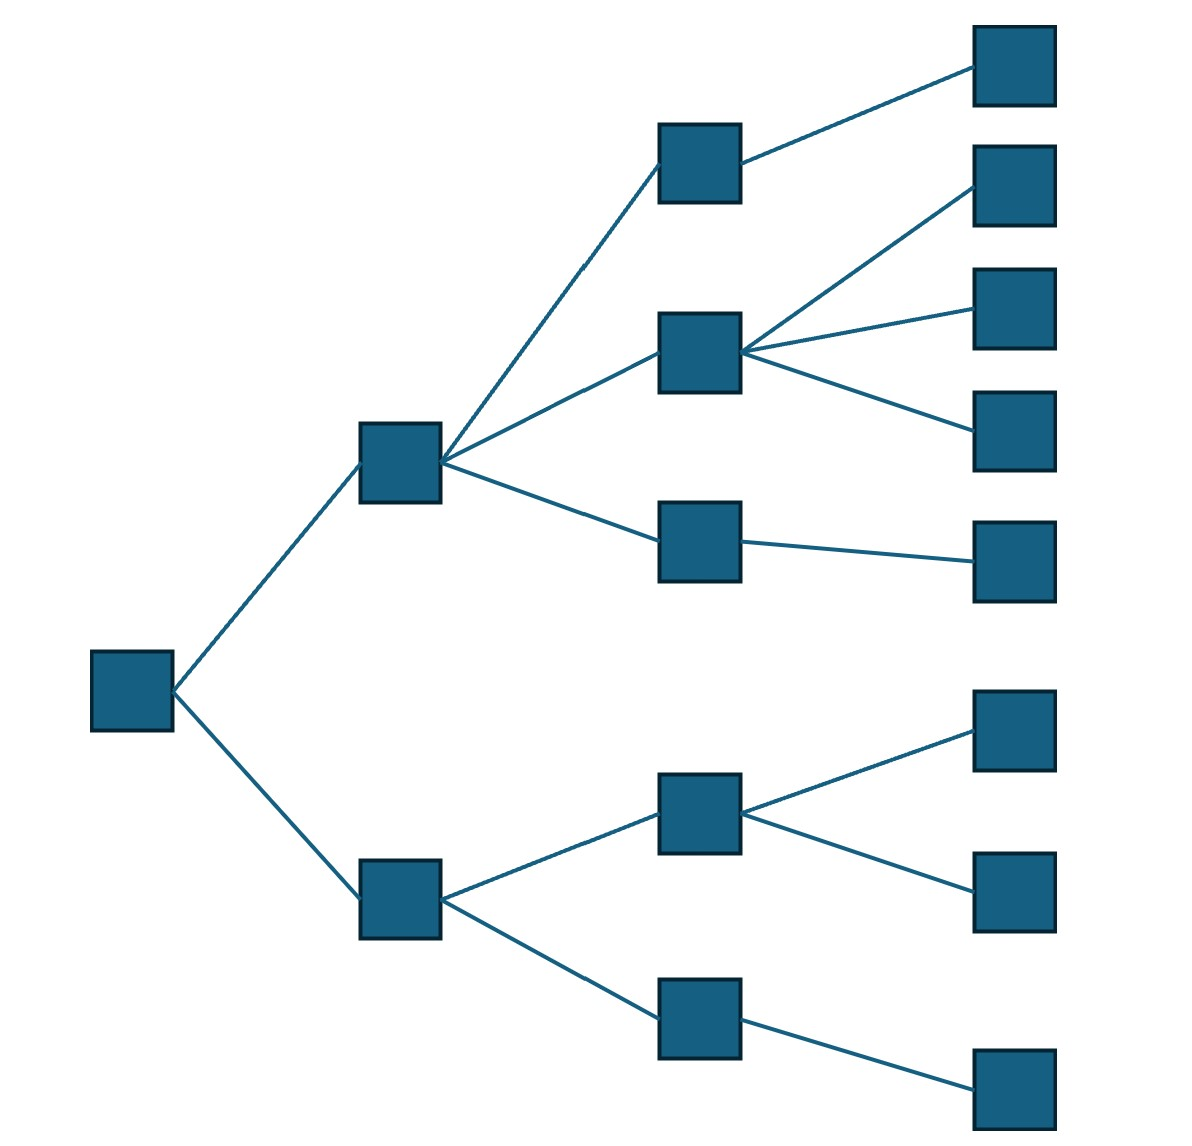
\includegraphics[height=6cm, width=7cm]{images/3-perioden-modell.jpg}
    \caption{Beispiel für einen Zustandsbaum}
    \label{fig:state-tree}
\end{figure}
\\Es sei $\Omega = \{ \omega_1, \ldots, \omega_m \}$ eine endliche Menge und $\mathbb{F}=(\mathcal{P}_0, \ldots, \mathcal{P}_N)$ eine Filtrierung von $\Omega$. Ein Zustandsbaum kann so aufgebaut werden, dass die $k$-te (vertikal stehende) Schicht aus den Blöcken der Partition $\mathcal{P}_k$ besteht. Abbildung \ref{fig:Filtrierung} zeigt ein Beispiel eines Zustandbaumes für eine Filtrierung. Im ersten Block links sind alle $\omega_i$ enthalten, womit die gesamte Menge $\Omega$ enthalten ist. Nach einem Schritt nach rechts enthält $B_{1,1}$ den ersten Teil und $B_{1,2}$ den zweiten Teil von $\Omega$.\footnote{$\Omega$ ist hierbei nicht unbedingt in zwei gleiche Teile aufgeteilt.} Nach einem weiteren Schritt nach rechts wird $B_{1,1}$ in zwei weitere Teile aufgeteilt, dasselbe gilt für $B_{1,2}$. Das geht so weiter, bis im letzten Schritt ganz rechts in jedem Block genau ein $\omega_i$ enthalten ist. Da im ersten Block ganz links die gesamte Menge $\Omega$ in einem Block und ganz rechts jedes $\omega\in\Omega$ seinen eigenen Block hat, ist diese Filtrierung gleichzeitig eine Informationsstruktur von $\Omega$.
\begin{figure}[h]
    \centering
    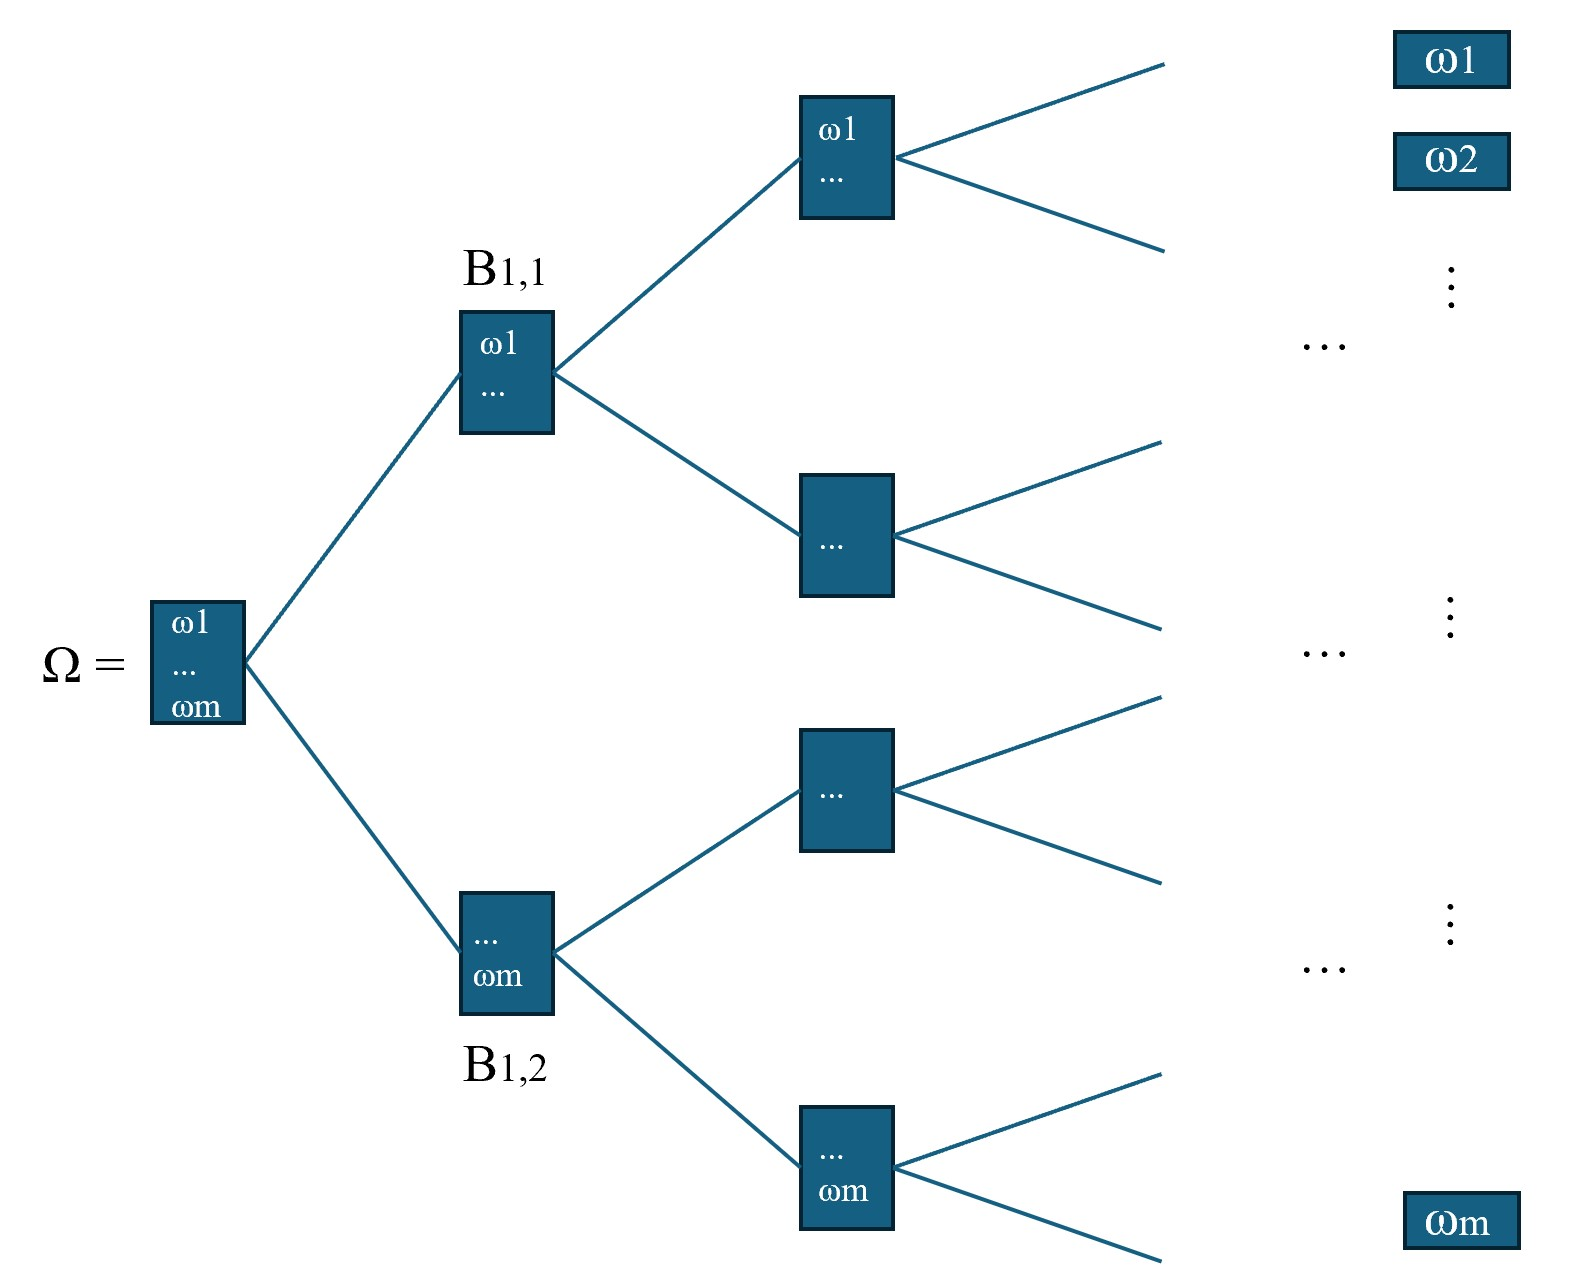
\includegraphics[width=15cm]{images/filtration.jpg}
    \caption{Eine Filtrierung und Informationsstruktur von $\Omega$}
    \label{fig:Filtrierung}
\end{figure}
\begin{Definition}{Informationsstruktur}{information-structure}
    Die Filtrierung $\mathbb{F}=(\mathcal{P}_0, \ldots, \mathcal{P}_N)$ von $\Omega=\{\omega_1, \ldots, \omega_n\}$ heisst Informationsstruktur, wenn $\mathcal{P}_0 = \{ \Omega \}$ und $\mathcal{P}_N = \{ \{\omega_1\}, \ldots, \{\omega_n\}\}$.
\end{Definition}
Betrachten wir den Kursverlauf einer Anlage, zum Beispiel einer Aktie. Der Ereignisraum $\Omega$ sei die (endliche) Menge aller Kursverläufe, die die Aktie während einer klar definierten Zeitdauer durchlaufen kann. Der Aktienpreis beginnt im Zustandsbaum im Block ganz links. Mit voranschreitender Zeit geht man im Zustandsbaum eine Schicht nach rechts. Stellt man sich eine Filtrierung von $\Omega$ vor, befindet sich in der ersten Partition $\mathcal{P}_0$ die gesamte Menge $\Omega$ der möglichen Aktienkursverläufe in einem einzigen Block. Da noch nichts mit dem Aktienpreis passiert ist, sind alle Kursverläufe immer noch möglich. Vergeht nun ein Teil der Zeit, passiert unter Umständen etwas mit dem Aktienkurs: Er könnte beispielsweise um 10\% steigen, um 12\% sinken oder aber einfach gleich bleiben. Es sind schliesslich nicht 
mehr alle Kursverläufe, welche zu Beginn möglich waren, erreichbar, da nun bereits etwas mit dem Aktienkurs passiert ist. Nach einem weiteren Zeitabschnitt verkleinert sich die Anzahl möglicher Kursverläufe pro Block weiter. In der letzten Partition $\mathcal{P}_N$ befindet sich in jedem vorhandenen Block genau ein möglicher Kursverlauf $\omega \in \Omega$. Diese Vorstellung ist grundlegend für das Verständnis des Binomialmodells und wird später noch genauer behandelt.

\section{Martingale}
\subsection{Nullsummenspiel}
Die Idee, die im Folgenden für die Herleitung der Binomialformeln zur Berechnung von Optionspreisen gebraucht wird, ist folgende: Wenn ein Käufer mit einer Aktie eine zu schlechte Aussicht auf Gewinn hätte, würde er die Aktie nie kaufen. Wenn ein Verkäufer mit der Aktie eine zu schlechte Aussicht auf Gewinn hätte, würde er sie nie verkaufen. Deshalb müssen die Preise so \textit{fair} sein, dass alle Beteiligten bereit sind, am Markt teilzunehmen (sprich: zu kaufen oder zu verkaufen). Dieses Konzept nennt man das \textit{No-Arbitrage-Prinzip}.\footnote{Mehr dazu auf Seite \pageref{def:no-arbitrage-principle}.}
\\Man überlegt sich am besten zwei Spieler, nennen wir sie Albert und Blaise, welche ein Spiel spielen. Sie werfen eine (gewichtete) Münze, Albert erhält bei \textit{Kopf} einen Franken, muss jedoch einen Franken zahlen, wenn die Münze auf \textit{Zahl} landet. Blaise hingegen erhält einen Franken bei \textit{Zahl} und verliert einen bei \textit{Kopf}. Die Wahrscheinlichkeit, dass die Münze auf \textit{Kopf} landet, ist $p$, dementsprechend ist die Wahrscheinlichkeit für \textit{Zahl} $1-p$. Albert würde nicht mitspielen, wenn sein erwarteter Gewinn kleiner als 0 wäre. Dasselbe gilt für Blaise. Die Spieler können jedoch auch nicht einen positiven erwarteten Gewinn haben, da so Geld \textit{aus dem Nichts} geschaffen würde. Das Spiel funktioniert also nur, wenn beide Spieler den erwarteten Gewinn $0$ haben. Der erwartete Gewinn für Albert ist $1\cdot p -1\cdot (1-p)$, was nur $0$ für $p=1/2$ ist.
\\Generalisiert: $X_0$ sei Alberts Gewinn vor dem ersten Münzwurf. $X_0$ ist zwingend $0$, weil ja noch nicht gespielt wurde. $X_1$ sei Alberts Gewinn nach dem ersten Münzwurf. $X_1$ ist entweder $-1$ oder $1$, weil er entweder gewinnt oder verliert. Bei $X_0$ und $X_1$ handelt es sich um Zufallsvariablen. Es muss gelten $$\mathcal{E}(X_1) = X_0 = 0$$
Alberts erwarteter Gewinn zum Zeitpunkt $t_1$ ist also gleich dem vorherigen Gewinn, die erwartete Gewinnveränderung beträgt 0: Es handelt sich um ein Nullsummenspiel.
\subsection{Verallgemeinerung}
Es sei $(\Omega, \mathbb{P})$ ein Wahrscheinlichkeitsraum. Wenn Albert und Blaise das Münzwurfspiel insgesamt $N$-mal spielen, ergeben die Zufallsvariablen $X_i$, welche Alberts Gewinn zum Zeitpunkt $t_i$ angeben, den stochastischen Prozess $$\mathbb{X}=(X_0, \ldots, X_N)$$ auf $\Omega$. $\mathbb{X}$ sei adaptiert auf die Filtrierung $\mathbb{F}=(\mathcal{P}_0, \ldots, \mathcal{P}_N)$ von $\Omega$. Hierbei gibt $\Omega$ die Menge aller möglicher Gewinnverläufe an.
\\Damit der stochastische Prozess $\mathbb{X}$ von jedem Spiel zum nächsten fair ist, muss also der bedingte erwartete Gewinn $X_{k+1}$ zum Zeitpunkt $t_{k+1}$, wobei der aktuelle Zustand $\mathcal{P}_k$ gegeben ist, gleich dem realisierten aktuellen Gewinn $X_k$ sein: $$\mathcal{E}(X_{k+1}|\mathcal{P}_k)=X_k$$ Ist das der Fall, nennt man den stochastischen Prozess $\mathbb{X}$ \textit{Martingal}.
\begin{Definition}{Martingal}{martingale}
    Es sei $(\Omega, \mathbb{P})$ ein endlicher Wahrscheinlichkeitsraum. Es sei $\mathbb{F}=(\mathcal{P}_0, \ldots, \mathcal{P}_N)$ eine Filtrierung von $\Omega$ und $\mathbb{X}=(X_0, \ldots, X_N)$ ein $\mathbb{F}$-adaptierter stochastischer Prozess. $\mathbb{X}$ ist ein Martingal bezüglich $(\Omega, \mathbb{P}, \mathbb{F})$, wenn
    $$\mathcal{E}(X_{k+1}|\mathcal{P}_k)=X_k$$ bzw. $$\mathcal{E}(\Delta_{k, k+1}(\mathbb{X})|\mathcal{P}_k)=0$$ wobei $\Delta_{k, k+1}(\mathbb{X})=X_{k+1}-X_{k}$.
\end{Definition}
Um mehr über Martingale herauszufinden, formuliert man folgendes Theorem:
\begin{Theorem}{Eigenschaften des bedingten Erwartungswerts}{exp-value-properties}
    Es sei $(\Omega, \mathbb{P})$ ein endlicher Wahrscheinlichkeitsraum, $\mathcal{P}=\{ B_1, \ldots, B_n\}$ eine Partition von $\Omega$, wobei für alle $i$ $\mathbb{P}(B_i)>0$
    \begin{enumerate}
        \item $\mathcal{E}(aX+bY|\mathcal{P})=a\mathcal{E}(X|\mathcal{P})+b\mathcal{E}(Y|\mathcal{P})$ wobei $X$ und $Y$ Zufallsvariablen und $a, b \in \mathbb{R}$.
        \item $\mathcal{E}(YX|\mathcal{P})=Y\mathcal{E}(X|\mathcal{P})$ wobei $Y$ eine $\mathcal{P}$-messbare Zufallsvariable ist.
        \item $\mathcal{E}(\mathcal{E}(X|\mathcal{P})|\mathcal{Q})=\mathcal{E}(X|\mathcal{P})=\mathcal{E}(\mathcal{E}(X|\mathcal{Q})|\mathcal{P})$ wobei $\mathcal{P}\succ\mathcal{Q}$. (Turmeigenschaft)
    \end{enumerate}
    Der Beweis findet sich im Anhang auf Seite \pageref{proof:towerprop}.
\end{Theorem}
Man kann damit übrigens auch den letzten Teil der Definition \ref{def:martingale} zeigen:
$$\mathcal{E}(\Delta_{k, k+1}(\mathbb{X})|\mathcal{P}_k)=\mathcal{E}(X_{k+1}-X_k|\mathcal{P}_k)=\mathcal{E}(X_{k+1}|\mathcal{P}_k)-\mathcal{E}(X_k|\mathcal{P}_k)=X_k-X_k=0\ \square$$
Aus Definition \ref{def:martingale} folgt, dass $$\mathcal{E}(X_k|\mathcal{P}_{k-1})=X_{k-1}$$
Wenn man den Erwartungswert bezüglich der Partition $\mathcal{P}_{k-2}$ nimmt, erhält man mithilfe der Turmeigenschaft $$\mathcal{E}(X_k|\mathcal{P}_{k-2})=\mathcal{E}(\mathcal{E}(X_k|\mathcal{P}_{k-1})|\mathcal{P}_{k-2})=\mathcal{E}(X_{k-1}|\mathcal{P}_{k-2})=X_{k-2}$$
Das kann man beliebig oft wiederholen und somit zeigen, dass für jedes $j<k$ gilt $$\mathcal{E}(X_k|\mathcal{P}_{j})=X_{j}$$ Das bedeutet, dass auch $$\mathcal{E}(X_N|\mathcal{P}_{0})=X_{0}$$
%\begin{Theorem}{Martingaleigenschaften}{martingale-props}
%Es sei $(\Omega, \mathbb{P})$ ein endlicher Wahrscheinlichkeitsraum, $\mathbb{F}=(\mathcal{P}_0, \ldots, \mathcal{P}_N)$ eine Filtrierung von $\Omega$ und $\mathbb{X}=(X_0, \ldots, X_N)$ ein $\mathbb{F}$-adaptierter stochastischer Prozess. Die folgenden Aussagen sind äquivalent:
%\begin{enumerate}
    %\item $\mathcal{E}(X_{k+1}|\mathcal{P}_{k})=X_{k}$
    %\item $\mathcal{E}(X_{k+i}|\mathcal{P}_{k})=X_{k}$
    %\item $\mathcal{E}(X_N|\mathcal{P}_{k})=X_{k}$
%\end{enumerate}
%\end{Theorem}

\section{Modelle mit diskreter Zeit}

Am einfachsten berechnet man Optionspreise so, indem man die Zeit in endlich viele Teile unterteilt und annimmt, dass alle Käufe und Verkäufe zu einem dieser Zeitpunkte stattfinden. Man nimmt die Zeit also als \textit{diskret} an.

\subsection{Annahmen}
In der Realität werden Aktienpreise durch unzählige Faktoren, wie spontane, menschliche Entscheidungen, politische Beschlüsse oder der Veröffentlichung von Geschäftsberichten, beeinflusst. Man kann unmöglich alle dieser unvorhersehbaren Einflüsse mathematisch berücksichtigen. Um ein Modell $\mathbb{M}$ zu erstellen, muss man also gewisse Annahmen machen, die die Situation vereinfachen.

\subsubsection*{Risikolose Anlagemöglichkeit}
Man nimmt an, dass es eine risikolose Anlagemöglichkeit gibt, welche im Zeitintervall $[t, t+\Delta t]$ um den Faktor $e^{r\Delta t}$ zulegt. $r$ nennt man den \textit{risikolosen Zinssatz}. Dafür werden Zinssätze genommen, die man auf sehr sichere Anlagemöglichkeiten erhält, beispielsweise auf Staatsanleihen.

\subsubsection*{Reibungsloser/Perfekter Markt}
Käufe und Verkäufe von Anlagen geschehen unverzüglich. Zudem existieren keine Transaktionsgebühren oder sonstige Kommissionen und keine Einschränkungen von Leerverkäufen.\footnote{Ein Leerverkauf funktioniert so, dass man eine Aktie verkauft, die man gar nicht besitzt, sondern nur ausleiht. Wenn der Aktienkurs später fällt, kann man die Aktie günstiger kaufen und zurückgeben. So hat man einen Gewinn gemacht, indem man auf einen fallenden Kurs gewettet hat (\cite{NZZ_2008}).}

\subsubsection*{Bid-Ask-Parität}
Wenn eine Anlage für den Preis $A$ gekauft werden kann, kann sie auch für denselben Preis $A$ verkauft werden. In der Realität sind diese Preise leicht unterschiedlich.

\subsubsection*{Unendlich teilbarer Markt}
Der Markt ist unendlich teilbar, wenn eine beliebige Anzahl Aktien erlaubt sind, beispielsweise $\displaystyle \frac{1}{e}$ oder $-2\sqrt{3}$.

\subsubsection*{Preise nach dem No-Arbitrage-Prinzip}
Man nimmt an, dass das sogenannte No-Arbitrage-Prinzip gilt. Arbitrage kann folgendermassen definiert werden:
\begin{Definition}{Arbitrage}{arbitrage}
    Eine Arbitrage-Möglichkeit ist eine Investitionsmöglichkeit, die mit Sicherheit keinen Verlust und wahrscheinlich Gewinn macht.
\end{Definition}
Wenn eine Arbitrage-Möglichkeit existiert, hat man also eine Aussicht auf Gewinn, ohne dass dabei eigenes Kapital eingesetzt wird. Dabei geht man davon aus, dass, wenn tatsächlich eine Arbitrage-Möglichkeit existiert, diese solange ausgenutzt wird, bis sich die entsprechenden Preise so angepasst haben, dass die Arbitrage-Möglichkeit verschwindet. Deshalb nimmt man einfachheitshalber an, dass grundsätzlich keine Arbitrage-Möglichkeiten existieren.
\begin{Definition}{No-Arbitrage-Prinzip}{no-arbitrage-principle}
    Bei der Berechnung von Anlagepreisen nimmt man an, dass keine Arbitrage-Möglichkeit existiert, weil der Markt dazu tendiert, Arbitrage-Möglichkeiten zu eliminieren. 
\end{Definition}

\subsubsection*{Zeit}
Im Modell existieren $T+1$ Zeitpunkte $$t_0<\ldots<t_T$$ und somit $T$ Zeitschritte/-intervalle $[t_{i-1}, t_i]$ für $i\leq T$.

\subsubsection*{Anlagen}
Man stellt sich vor, dass man zwei Anlagen besitzen kann:
\begin{itemize}
    \item $\mathfrak{a}_1$ ist die risikolose Anlage, welche im Zeitintervall $[t, t+\Delta t]$ um den Faktor $e^{r\Delta t}$ (risikoloser Zinssatz) wächst.
    \item $\mathfrak{a}_2$ ist die risikobehaftete/riskante Anlage, zum Beispiel eine Aktie.
\end{itemize}

\subsubsection*{Zustände}
Zum Zeitpunkt $t_T$ befinden sich die Anlagen in einem von $m$ möglichen Zuständen (jede Anlage hat einen bestimmten Preis), welche durch den Ergebnisraum $$\Omega=\{ \omega_1, \ldots, \omega_m\}$$ gegeben sind. Die Informationsstruktur $$\mathbb{F}=(\mathcal{P}_0, \ldots, \mathcal{P}_T)$$ von $\Omega$ nennt man die Informationsstruktur des Modells $\mathbb{M}$. In jedem Block $B_{i, j}$ befinden sich die Gesamtkursverläufe, die, ausgehend von $B_{i, j}$, theoretisch noch möglich sind. Im Block $B_{0,1}$ befindet sich die gesamte Menge $\Omega$, da man erst am Anfang steht und deshalb noch alles möglich ist. Im Block $B_{T, 1}$ hingegen befindet sich nur noch ein Gesamtkursverlauf, da man sich am Ende der Zeitdauer befindet und deshalb kein anderer als der aktuelle Kursverlauf erreichbar ist.\\Die Partition $$\mathcal{P}_i = \{ B_{i, 1}, \ldots, B_{i, m_i}\}$$ sei die Zustandspartition zur Zeit $t_i$ und für $i<T$ seien die Blöcke von $\mathcal{P}_i$ die Zwischenzustände zur Zeit $t_i$. Abbildung \ref{fig:zustandsbaum_M} zeigt den Zustandsbaum des Modells $\mathbb{M}$:
\begin{figure}[h]
    \centering
    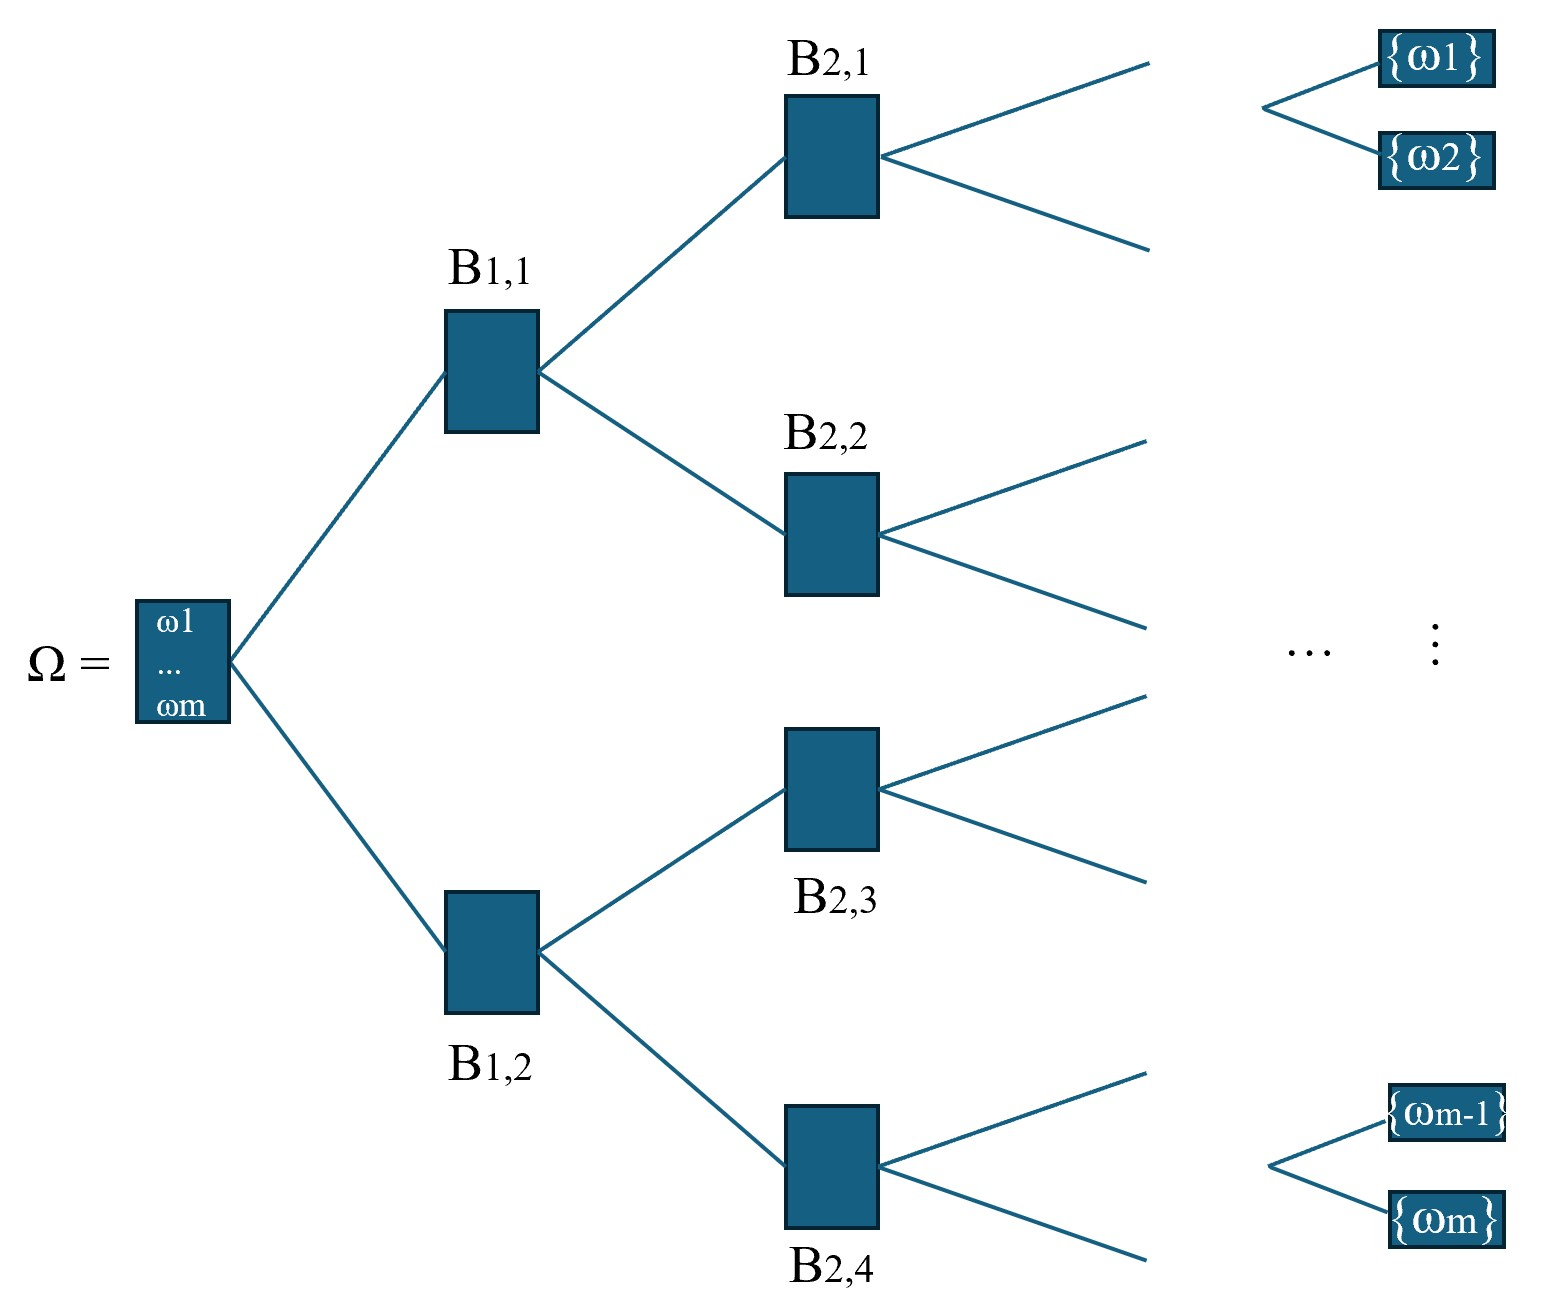
\includegraphics[height=12cm]{images/zustandsbaum_M.jpg}
    \caption{Zustandsbaum des Modells}
    \label{fig:zustandsbaum_M}
\end{figure}

\subsubsection*{Wahrscheinlichkeiten}
Es gebe für jeden möglichen Endzustand $\omega \in \Omega$ eine Wahrscheinlichkeit, die angibt, wie wahrscheinlich es ist, dass $\omega$ eintrifft. 

\subsection{Anlagepreise}
\begin{Definition}{Anlagepreise}{asset-prices}
    \begin{enumerate}
        \item Für jede Zeit $t_i$ und jeden der beiden Anlagen $\mathfrak{a}_j$ gibt es die Zufallsvariable $$S_{i, j}:\Omega \mapsto \mathbb{R}$$ für die $S_{i, j}(\omega)$ den Preis der Anlage $\mathfrak{a}_j$ zum Zeitpunkt $t_i$ für den Endzustand $\omega$ angibt.
        \item Die Folge $$\mathbb{S}_j=(S_{0, j}, \ldots, S_{T, j})$$ ist ein stochastischer Prozess, der die Preisentwicklung der Anlage $\mathfrak{a}_j$ über die Zeit angibt. Man nennt ihn \textit{Preisprozess}.
        \item Da die risikolose Anlage $\mathfrak{a}_1$ mit dem risikolosen Zinssatz $r$ wächst, ist $$S_{0, 1}=1$$ und für alle $i>0$ $$S_{i, 1}=e^{r(t_i-t_0)}$$
    \end{enumerate}
\end{Definition}
\begin{Definition}{Abzinsung}{discounting}
    Um den Wert $A_i$ zur Zeit $t_i$ abzuzinsen, also um auf den äquivalenten Wert $\overline{A}_i$ zur Zeit $t_0$ zu kommen, benutzt man den risikolosen Zinssatz:
    \begin{align*}
        \overline{A}_i&=A_ie^{-r(t_i-t_0)}\\
        &= A_i(S_{i, 1})^{-1}\\
        &= \frac{A_i}{S_{i, 1}}
    \end{align*}
\end{Definition}
\subsection{Portfolios und Handelsstrategien}
\begin{Definition}{Portfolio und Anlagehalteprozess}{portfolio-asset-holding-process}
    \begin{enumerate}
        \item $\theta_{i, j}$ sei eine Zufallsvariable, sodass $\theta_{i, j}(\omega)$ angibt, wie viele Einheiten der Anlage $\mathfrak{a}_j$ man während dem Zeitintervall $[t_{i-1}, t_i]$ für den Endzustand $\omega$ besitzt.
        \item Der Anlagehalteprozess für die Anlage $\mathfrak{a}_j$ ist der stochastische Prozess $$\Phi_j=(\theta_{1, j}, \ldots, \theta_{T, j})$$
        \item Das Portfolio für das Zeitintervall $[t_{i-1}, t_i]$ ist $$\Theta_i=(\theta_{i, 1}, \theta_{i, 2})$$
    \end{enumerate}
\end{Definition}
 \begin{Beispiel}{}{}
     $\Phi_2=(3, 4)$ bedeutet, dass man während dem Intervall $[t_0, t_1]$ 3 Einheiten und während dem Intervall $[t_1, t_2]$ 4 Einheiten der Anlage $\mathfrak{a}_2$ besitzt.
 \end{Beispiel}
\begin{Beispiel}{}{}
    $\Theta_3=(29, 5)$ bedeutet, dass man  während dem Intervall $[t_2, t_3]$ 29 Einheit der risikolosen Anlage $\mathfrak{a}_1$ und 5 Einheiten der risikobehafteten Anlage $\mathfrak{a}_2$ besitzt.
\end{Beispiel}
 Zu den Zeitpunkten $t_k$ können Anlagen verkauft oder gekauft werden, es kann auch gar nichts damit gemacht werden und sie können somit unverändert gelassen werden. Man stellt es sich trotzdem am besten so vor, dass zu jedem Zeitpunkt $t_k$ das ganze Portfolio verkauft (\textit{liquidiert}) und danach ein neues Portfolio gekauft (\textit{akquiriert}) wird. Auch wenn man gar nichts am Portfolio ändern will, verkauft man das ganze Portfolio und kauft es darauf in der exakt gleichen Form wieder ein.\footnote{In Wirklichkeit würde dies keinen Sinn machen, da man für jeden Kauf und Verkauf Transaktionsgebühren bezahlt. Da jedoch der Einfachheit halber angenommen wurde, dass man keine Transaktionsgebühren bezahlen muss (reibungsloser Markt), kann man hier trotzdem so vorgehen.}
 \begin{Definition}{Handelsstrategie}{trading-strat}
     Für ein Modell $\mathbb{M}$ nennt man die Folge $$\Phi=(\Theta_1, \ldots, \Theta_T)$$ -- bzw. die Entwicklung des Portfolios $\Theta$ über die Zeit -- eine \textit{Handelsstrategie}.
 \end{Definition}
Es liegt auf der Hand, anzunehmen, dass am Anfang ($t_0$) eine gewisse Menge Geld in das Portfolio $\Theta_1$ investiert wird und während jeder Liquidation und Akquisition kein Geld aus dem Portfolio herausgenommen wird und kein neues Geld dazukommt.
\\Der Akquisitionspreis des Portfolios $\Theta_i$ sei definiert als\footnote{Ich arbeite hier nur mit zwei Anlagen ($\mathfrak{a}_1$ und $\mathfrak{a}_2$), theoretisch könnte man aber beliebig viele Anlagen verwenden, dann würde man beim Summenzeichen "2" \ durch die entsprechende Anzahl Anlagen ersetzen.} $$\mathcal{V}_{i-1}(\Theta_i)=\sum_{j=1}^{2}\theta_{i, j}S_{i-1, j}=\theta_{i, 1}S_{i-1, 1}+\theta_{i, 2}S_{i-1, 2}$$
Der Liquidationspreis des Portfolios $\Theta_i$ sei definiert als $$\mathcal{V}_{i}(\Theta_i)=\sum_{j=1}^{2}\theta_{i, j}S_{i, j}=\theta_{i, 1}S_{i, 1}+\theta_{i, 2}S_{i, 2}$$
Es wird also weder Geld aus dem Portfolio herausgenommen noch neues Geld dazugetan, wenn der Akquisitionspreis des neuen Portfolios $\Theta_{i+1}$ gleich gross wie der Liquidationspreis des alten Portfolios $\Theta_i$ ist. Man nennt eine solche Handelsstrategie \textit{selbstfinanzierend}.
\begin{Definition}{Selbstfinanzierende Handelsstrategie}{self-financing-trading-strat}
Eine Handelsstrategie $\Phi=(\Theta_1, \ldots, \Theta_T)$ ist selbstfinanzierend, wenn für alle Zeiten $t_i$, wobei $0<i<T$, gilt $$\mathcal{V}_i(\Theta_{i+1})=\mathcal{V}_i(\Theta_i)$$
\end{Definition}
Da also bei selbstfinanzierenden Handelsstrategien $\Phi$ der Liquidationspreis von $\Theta_i$ gleich dem Akquisitionspreis von $\Theta_{i+1}$ ist, kann man verallgemeinert schreiben $$\mathcal{V}_i(\Theta_{i+1})=\mathcal{V}_i(\Theta_i)=:\mathcal{V}_i(\Phi)$$
Zinst man die Portfoliopreise ab, erhält man $$\overline{\mathcal{V}}_{i}(\Phi)=\overline{\mathcal{V}}_{i}(\Theta_i)=\sum_{j=1}^{2}\theta_{i, j}\overline{S}_{i, j}=\frac{\mathcal{V}_i(\Theta_i)}{S_{i, 1}}$$
\begin{Definition}{Wertprozess}{value-process}
    Der stochastische Prozess $$\mathbb{V}=(\mathcal{V}_0(\Phi), \ldots, \mathcal{V}_T(\Phi))$$ heisst Wertprozess von $\Phi$. Der stochastische Prozess $$\overline{\mathbb{V}}=(\overline{\mathcal{V}}_0(\Phi), \ldots, \overline{\mathcal{V}}_T(\Phi))$$ heisst abgezinster Wertprozess von $\Phi$.
\end{Definition}
\section{Martingalmasse}
\begin{Definition}{Abgezinster Zuwachs}{discounted-gain}
    Es sei $\Phi$ eine selbstfinanzierende Handelsstrategie. 
    \begin{enumerate}
        \item Für $j<k$ heisst $$\overline{G}_{j, k}(\Phi)=\overline{\mathcal{V}}_k(\Phi)-\overline{\mathcal{V}}_j(\Phi)=\frac{\mathcal{V}_k(\Phi)}{S_{k, 1}}-\frac{\mathcal{V}_j(\Phi)}{S_{j, 1}}$$ abgezinster Zuwachs $\overline{G}_{j, k}$ von $t_j$ bis $t_k$.
        \item Für jedes $t_k$ heisst $$\overline{G}_{k}(\Phi)=\overline{\mathcal{V}}_k(\Phi)-\overline{\mathcal{V}}_0(\Phi)$$ kumulativer abgezinster Zuwachs von $\Phi$.
    \end{enumerate}
\end{Definition}
\begin{Definition}{Martingalmass}{martingale-meas}
    Es sei $\mathbb{M}$ ein Modell mit diskreter Zeit mit der Informationsstruktur $\mathbb{F}=(\mathcal{P}_0, \ldots, \mathcal{P}_T)$. Ein Wahrscheinlichkeitsmass $\mathbb{P}$ auf $\Omega$ ist ein Martingalmass für $\mathbb{M}$, wenn
    \begin{enumerate}
        \item für alle $\omega \in \Omega$ gilt $$\mathbb{P}(\omega)>0$$
        \item für jede Anlage $\mathfrak{a}_j$ der abgezinste Preisprozess $(\overline{S}_{0, j}, \ldots, \overline{S}_{T, j})$ ein Martingal ist. Das heisst, dass für alle $k\geq0$ $$\mathcal{E}_{\mathbb{P}}(\overline{S}_{k+1, j}|\mathcal{P}_{k})=\overline{S}_{k, j}$$
    \end{enumerate}
\end{Definition}
\begin{Beispiel}{}{}
    Man stellt sich ein Ein-Perioden-Modell vor. Eine Aktie kann also nur vom Zeitpunkt $t_0$ bis $t_1$ ihren Wert verändern. Der Aktienpreis steigt oder er fällt. Bei $t_0$ beträgt der Aktienpreis \$100. Bis $t_1$ ist der Preis entweder auf \$200 gestiegen oder auf \$50 gefallen. Das Wahrscheinlichkeitsmass $$\mathbb{P}(\text{steigt})=\frac{1}{3}, \mathbb{P}(\text{fällt})=\frac{2}{3}$$ ist ein Martingalmass, weil der erwartete Aktienpreis zum Zeitpunkt $t_1$ gleich dem Aktienpreis zum Zeitpunkt $t_0$ ist: $$\frac{1}{3}\cdot \$200 + \frac{2}{3}\cdot \$50=\$100$$
\end{Beispiel}
\subsection{Eigenschaften von Martingalmassen}
Man stelle sich ein Portfolio $\Theta$ vor, das zu Beginn leer ist, also keine einzige Anlage beinhaltet. Im Falle des Zustands $B \in \mathcal{P}_k$ leiht man sich zum Zeitpunkt $t_k$ genau so viel Geld (bzw. risikolose Anlage $\mathfrak{a}_1$),\footnote{Bzw. man macht einen Leerverkauf von Anlage $\mathfrak{a}_1$.} wie für eine Einheit der risikobehafteten Anlage $\mathfrak{a}_2$ gebraucht wird und kauft dann eine Einheit von $\mathfrak{a}_2$. Im nächsten Schritt verkauft man $\mathfrak{a}_2$ wieder. Anders formuliert hat man kein Startkapital und kauft, falls man sich im Zustand $B$ befindet, mit geliehenem Geld die Anlage $\mathfrak{a}_2$ und verkauft sie zum nächstmöglichen Zeitpunkt wieder. Diese Handelsstrategie nennt man \textit{atomare Handelsstrategie}.
\begin{Definition}{Atomare Handelsstrategien}{atomic-trading-strat}
    Die Handelsstrategie
    $$\Theta_i=\begin{cases}
        (0,0) & \text{falls } 1\leq i \leq k\\  
        (-\overline{S}_{k, 2}, 1)1_B & \text{falls } i=k+1\\
        (-\overline{S}_{k, 2}+\overline{S}_{k+1, 2}, 0)1_B & \text{falls } k+1<i\leq T
    \end{cases}$$ heisst atomare Handelsstrategie $\Phi[\mathfrak{a}_2, t_k, B]$.
\end{Definition}
Der gesamte kumulative abgezinste Zuwachs einer atomaren Handelsstrategie ist demnach gleich der abgezinsten Preisänderung der Anlage $\mathfrak{a}_2$ von $t_k$ bis $t_{k+1}$ im Zustand $B$: \begin{equation} \label{eq:blablibu}
    \overline{G}_T(\Phi[\mathfrak{a}_2, t_k, B])=\overline{G}_{k, k+1}(\Phi[\mathfrak{a}_2])1_B=\Delta_{k, k+1}(\overline{\mathbb{S}}_2)1_B
\end{equation}
Für das Wahrscheinlichkeitsmass $\mathbb{P}$ gelte für alle $\omega \in \Omega$, dass $\mathbb{P}(\omega)>0$. Gemäss Definition \ref{def:martingale-meas} ist $\mathbb{P}$ genau dann ein Martingalmass, wenn für alle Anlagen $\mathfrak{a}_j$, Zeitpunkte $t_k$ und Zustände $B \in \mathcal{P}_k$ gilt, dass $$\mathcal{E}(\overline{S}_{k+1, j}|B)=\overline{S}_{k, j}(B)$$ wobei $0 \leq k < T$, bzw. \begin{equation}\label{eq:hundsverlochete}
    \mathcal{E}(\Delta_{k, k+1}(\overline{\mathbb{S}}_j)|B)=0 
\end{equation}
Gleichung \ref{eq:blablibu} zeigt, dass 
$$\mathcal{E}(\overline{G}_T(\Phi[\mathfrak{a}_2, t_k, B]))=\mathcal{E}(\Delta_{k, k+1}(\overline{\mathbb{S}}_2)1_B)=\mathbb{P}(B)\mathcal{E}(\Delta_{k, k+1}(\overline{\mathbb{S}}_2)|B)$$
Kombiniert man mit Gleichung \ref{eq:hundsverlochete}, erhält man also 
$$\mathcal{E}(\overline{G}_T(\Phi[\mathfrak{a}_2, t_k, B]))=\mathbb{P}(B)\cdot0=0 $$

\begin{Theorem}{}{martingale-meas-atom-trad-strat}
    Es sei $\mathbb{M}$ ein Modell mit diskreter Zeit und der Informationsstruktur $\mathbb{F}=(\mathcal{P}_0, \ldots, \mathcal{P}_T)$. Ein Wahrscheinlichkeitsmass $\mathbb{P}$ (wobei $\mathbb{P}(\omega)>0$ für alle $\omega \in \Omega$) ist genau dann ein Martingalmass, wenn $$\mathcal{E}_{\mathbb{P}}(\overline{G}_T(\Phi[\mathfrak{a}_2, t_k, B]))=0$$ für alle Zeitpunkte $t_k$ und Zustände $B \in \mathcal{P}_k$, wobei $k<T$.
\end{Theorem}
Laut seiner Definition ist $\mathbb{P}$ (wobei $\mathbb{P}(\omega)>0$ für alle $\omega \in \Omega$) genau dann ein Martingalmass, wenn alle abgezinsten Preisprozesse $\overline{\mathbb{S}}_j$ Martingale sind. Ebenso ist $\mathbb{P}$ genau dann ein Martingalmass, wenn alle abgezinsten Wertprozesse $$(\overline{\mathcal{V}}_0(\Phi), \ldots, \overline{\mathcal{V}}_T(\Phi))$$ für selbstfinanzierende Handelsstrategien $\Phi$ Martingale sind. Zweiteres zeigt man folgendermassen:
\\Angenommen, $\mathbb{P}$ ist ein Martingalmass. Dann gilt für jeden Wertprozess $(\overline{\mathcal{V}}_0(\Phi), \ldots, \overline{\mathcal{V}}_T(\Phi))$
\begin{align*}
    \mathcal{E}_\mathbb{P}(\overline{\mathcal{V}}_{k+1}(\Phi)|\mathcal{P}_k) 
    &= \mathcal{E}_\mathbb{P}(\theta_{k+1, 1}\overline{S}_{k+1, 1}+\theta_{k+1, 2}\overline{S}_{k+1, 2}|\mathcal{P}_k)\\
    &= \mathcal{E}_\mathbb{P}(\theta_{k+1, 1}\overline{S}_{k+1, 1}|\mathcal{P}_k)+\mathcal{E}_\mathbb{P}(\theta_{k+1, 2}\overline{S}_{k+1, 2}|\mathcal{P}_k)\\
    &= \theta_{k+1, 1}\mathcal{E}_\mathbb{P}(\overline{S}_{k+1, 1}|\mathcal{P}_k)+\theta_{k+1, 2}\mathcal{E}_\mathbb{P}(\overline{S}_{k+1, 2}|\mathcal{P}_k)\\
    &= \theta_{k+1, 1}\overline{S}_{k, 1}+\theta_{k+1, 2}\overline{S}_{k, 2}\\
    &= \overline{\mathcal{V}}_k(\Phi)
\end{align*}
und somit ist bewiesen, dass die abgezinsten Wertprozesse Martingale sind. 
Wenn die abgezinsten Wertprozesse Martingale sind, dann gilt auch

$$\mathcal{E}(\overline{\mathcal{V}}_{k}(\Phi)|\mathcal{P}_k) = \overline{\mathcal{V}}_0(\Phi)$$
bzw.$$\mathcal{E}(\overline{G}_k(\Phi))=0$$
und somit (wie früher gezeigt) auch$$\mathcal{E}(\overline{G}_T(\Phi))=0$$
$\Phi$ sei nun die atomare Handelsstrategie $\Phi[\mathfrak{a}_2, t_k, B]$, womit laut Theorem \ref{th:martingale-meas-atom-trad-strat} $\mathbb{P}$ ein Martingalmass ist.\ 
\begin{Theorem}{Eigenschaften von Martingalmassen}{martingale-meas-props}
    Es sei $\mathbb{M}$ ein Modell mit diskreter Zeit und der Informationsstruktur $\mathbb{F}=(\mathcal{P}_0, \ldots, \mathcal{P}_T)$. Für ein Wahrscheinlichkeitsmass $\mathbb{P}$ (wobei $\mathbb{P}(\omega)>0$ für alle $\omega \in \Omega$) sind folgende Aussagen äquivalent:
    \begin{enumerate}
        \item $\mathbb{P}$ ist ein Martingalmass, es gilt also für jedes $j<n$ $$\mathcal{E}_\mathbb{P}(\Delta_{k, k+1}(\overline{\mathbb{S}})|\mathcal{P}_k)=0$$
        \item Der abgezinste Wertprozess $(\overline{\mathcal{V}}_0(\Phi), \ldots, \overline{\mathcal{V}}_T(\Phi))$ ist für jede selbstfinanzierende Handelsstrategie ein Martingal.
        \item Der erwartete abgezinste Zuwachs von $t_0$ bis $t_k$ (wobei $k \leq T$) ist für jede selbstfinanzierende Handelsstrategie $\Phi$ gleich null: $$\mathcal{E}_\mathbb{P}(\overline{G}_k(\Phi))=0$$
        \item Der erwartete Gesamtzuwachs ($t_0$ bis $t_T$) ist für jede atomare Handelsstrategie 0: $$\mathcal{E}_\mathbb{P}(\overline{G}_k(\Phi[\mathfrak{a}_2, t_k, B]))=0$$ für alle Zeitpunkte $t_k$ und Zustände $B \in \mathcal{P}_k$ und $k<T$.
    \end{enumerate}
\end{Theorem}

\subsection{Martingalmasse berechnen}
\begin{Theorem}{Erster Fundamentalsatz der Arbitragepreistheorie}{fund-th-arb-theory}
    Ein Modell mit diskreter Zeit $\mathbb{M}$ hat genau dann keine Arbitragemöglichkeiten, wenn es ein Martingalmass hat und $\mathbb{P}(\omega)>0$ für alle $\omega\in\Omega$.\\\\(Der Beweis ist sperrig und befindet sich deshalb im Anhang auf Seite \pageref{proof:fund-th-arb-theo}.)
\end{Theorem}
\begin{figure}[h]
    \centering
    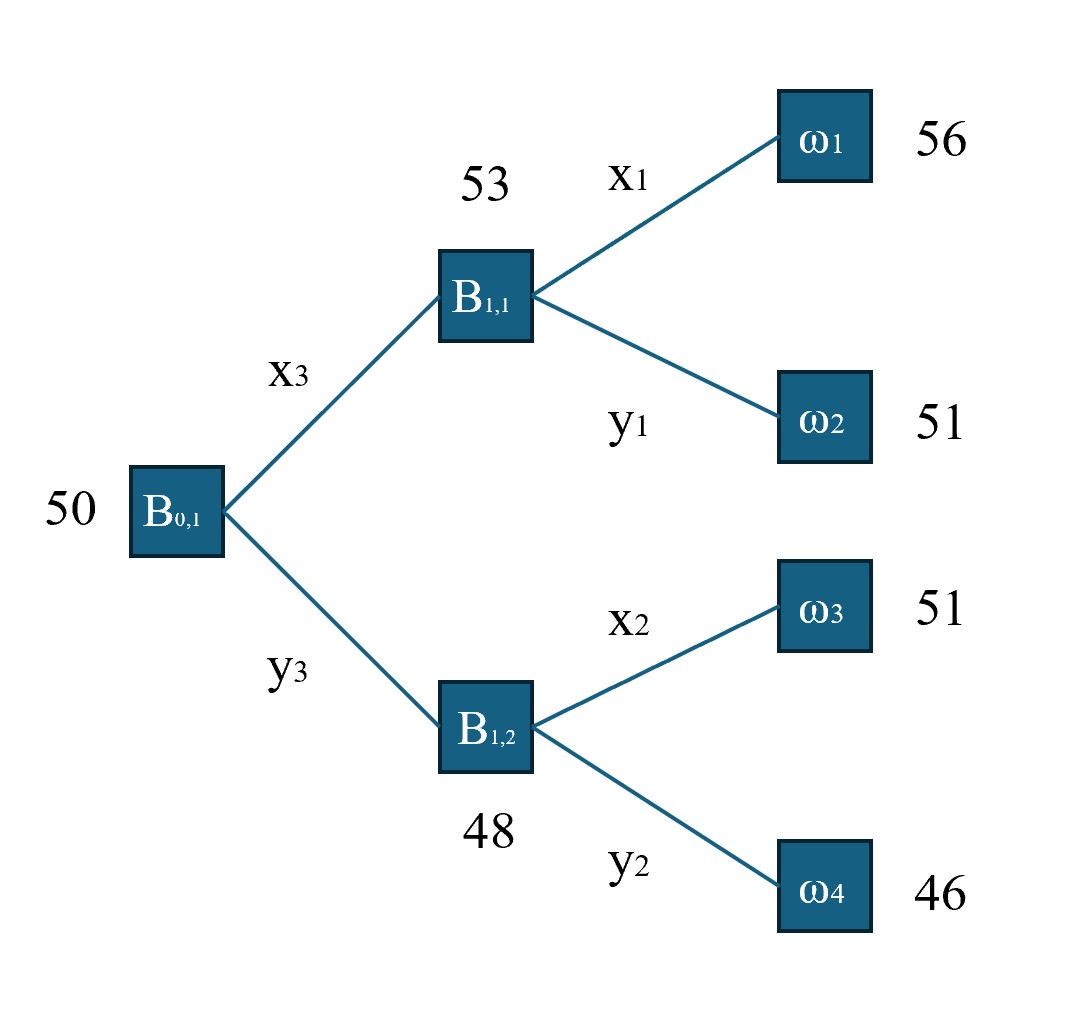
\includegraphics[width=7cm]{images/mart-prob-tree-unslvd.jpg}
    \caption{Zustandsbaum für ein Modell mit diskreter Zeit}
    \label{fig:mart-prob-tree-unsolved}
\end{figure}
Abbildung \ref{fig:mart-prob-tree-unsolved} zeigt den Zustandsbaum für ein Modell mit diskreter Zeit. Bei den Knoten steht der Aktienpreis für den jeweiligen Zustand. Über den Verbindungslinien zu den nächsten Zuständen stehen die Wahrscheinlichkeiten $x_i$ dafür, dass der Aktienpreis steigt bzw. $y_i$ dafür, dass der Aktienpreis sinkt. Das heisst, dass der Aktienpreis im Beispiel während dem ersten Zeitintervall von 50 mit der Wahrscheinlichkeit $x_3$ auf 53 steigt und mit der Wahrscheinlichkeit $y_3$ auf 48 sinkt. Dabei wird angenommen, dass der risikolose Zinssatz 0 beträgt.\\
Es ist logisch, dass \begin{align}\label{eq:uno}1=x_i+y_i\end{align} wenn sich der Aktienpreis nur in zwei Richtungen bewegen kann. Wenn $\mathcal{P}_k=\{B_{k,1},\ldots,B_{k,c}\}$ die Partition von $\Omega$ zum Zeitpunkt $t_k$ ist, lassen sich die Wahrscheinlichkeiten -- allgemein $p$ genannt -- auch folgendermassen schreiben:
$$p=\mathbb{P}(B_{k+1, i}|B_k)$$ womit sich die Martingalbedingung $$\mathcal{E}(\overline{S}_{k+1, j}|B_k)=\overline{S}_{k, j}(B_k)$$ als \begin{align}\label{eq:due}\overline{S}_{k, j}(B_k)=\sum_{i=1}^{2}\overline{S}_{k+1, j}(B_{k+1, i})\mathbb{P}(B_{k+1, i}|B_k)\end{align} schreiben lässt.\ 
\begin{Theorem}{}{calculation-mart-meas}
    Es sei $\mathbb{M}$ ein Modell mit diskreter Zeit. Wenn die Verbindungslinien im Zustandsbaum mit den Wahrscheinlichkeiten $p=\mathbb{P}(B_{k+1, i}|B_k)>0$ beschriftet sind, bilden diese genau dann ein Martingalmass, wenn die Gleichungen \ref{eq:uno} und \ref{eq:due} stimmen.
\end{Theorem}
Nun kann man die Gleichungen \ref{eq:uno} und \ref{eq:due} brauchen, um die Wahrscheinlichkeiten des Martingalmasses im Beispiel in Abbildung \ref{fig:mart-prob-tree-unsolved} zu berechnen:
\begin{equation*}
    \begin{cases}
        x_1+y_1&=1\\
        56x_1+51y_1&=53
    \end{cases}
\end{equation*}
hat die Lösung $x_1=\frac{2}{5}, y_1=\frac{3}{5}$. Auf dieselbe Art berechnet man die anderen Wahrscheinlichkeiten:
\begin{equation*}
    \begin{cases}
        x_2+y_2&=1\\
        51x_2+46y_2&=48
    \end{cases}
\end{equation*}
hat die Lösung $x_2=\frac{2}{5}, y_2=\frac{3}{5}$ und 
\begin{equation*}
    \begin{cases}
        x_3+y_3&=1\\
        53x_3+48y_3&=50
    \end{cases}
\end{equation*}
hat die Lösung $x_3=\frac{2}{5}, y_3=\frac{3}{5}$.
\\Abbildung \ref{fig:mart-prob-tree-unsolved} kann man jetzt ausfüllen:
\begin{figure}[h]
    \centering
    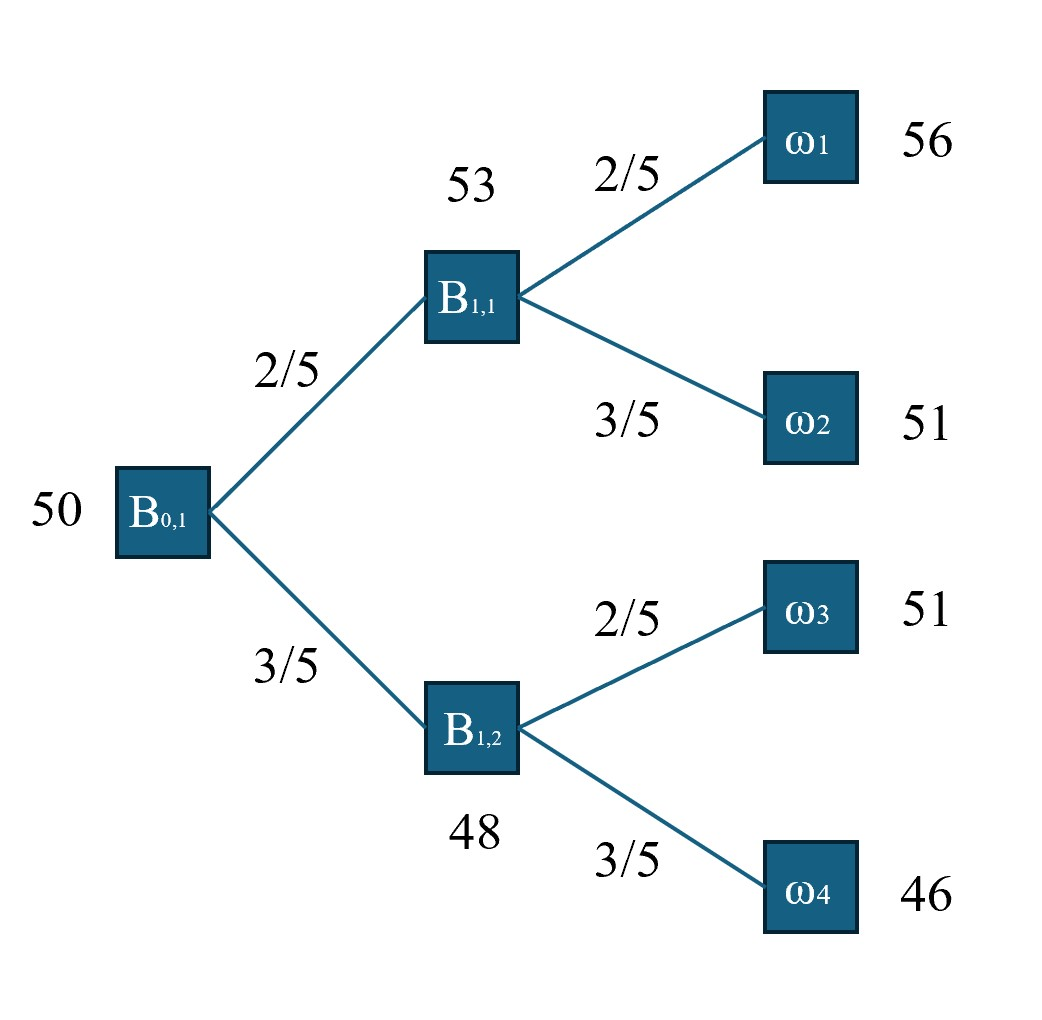
\includegraphics[width=7cm]{images/mart-prob-tree-slvd.jpg}
    \caption{Zustandsbaum mit Wahrscheinlichkeiten}
    \label{fig:mart-prob-tree-slvd}
\end{figure}
\\So kann man auch die Wahrscheinlichkeiten für jeden einzelnen Endzustand berechnen\label{compute-mart-probs}:
\begin{align*}\label{compute-mart-probs}
    &\mathbb{P}(\omega_1)=2/5\cdot2/5=\frac{4}{25}\\
    &\mathbb{P}(\omega_2)=2/5\cdot3/5=\frac{6}{25}\\
    &\mathbb{P}(\omega_3)=3/5\cdot2/5=\frac{6}{25}\\
    &\mathbb{P}(\omega_4)=3/5\cdot3/5=\frac{9}{25}
\end{align*}
Somit gibt es ein Martingalmass für dieses Modell und laut dem ersten Fundamentalsatz der Arbitragepreistheorie ist das Modell somit auch frei von Arbitrage.

\subsection{Alternativen und Replikation}
Bisher wurde hier einfach die Entwicklung von Aktienpreisen betrachtet, wenn man jedoch Optionspreise berechnen will, muss man eigentlich eine Zufallsvariable berechnen, die vom Aktienpreis abhängt. Der Payoff $X$ einer Call-Option mit Ausübungspreis $K$ am Ende der Laufzeit beträgt, wie früher schon behandelt, $$X=(S_T-K)^+$$ bzw. für eine Put-Option $$X=(K-S_T)^+$$Die Optionen haben somit zum Zeitpunkt $t_T$ den Wert $(S_T-K)^+$ bzw. $(K-S_T)^+$. Es gilt also, den Payoff bzw. Wert der Option auf den Zeitpunkt des Optionskaufs zurückzurechnen/zu schätzen.
\begin{Beispiel}{}{}
    Eine Call-Option mit Ausübungspreis $K=50$ und $S_T=75$ hat zum Zeitpunkt $t_T$ den Payoff $$(75-50)^+=(25)^+=25$$
\end{Beispiel}
\begin{Beispiel}{}{}
     Eine Call-Option mit Ausübungspreis $K=50$ und $S_T=45$ hat den Payoff $$(45-50)^+=(-5)^+=0$$
\end{Beispiel}
\begin{Definition}{Alternative}{alternative}
    Eine Zufallsvariable $X:\Omega \mapsto \mathbb{R}$ nennt man auch \textit{Alternative}.
\end{Definition}
Der \textit{finale Payoff} (bzw. Wert der Option zum Zeitpunkt $t_T$) ist somit auch eine Alternative. Er ist nicht gleich dem Aktienpreis, sondern hängt von diesem ab, er kann also vom Aktienpreis abgeleitet\footnote{Deshalb nennt man Finanzinstrumente, deren Preis vom Aktienpreis abgeleitet wird (wie z. B. Optionen), auch \textit{Derivate}.} werden.
\\\\Die Idee, um die Alternative $X$ zu berechnen, ist, eine selbstfinanzierende Handelsstrategie $\Phi$ zu finden, für die gilt $$\mathcal{V}_T(\Phi)=X$$
\begin{Theorem}{Gesetz des Einheitspreises}{law-of-one-price}
    Für alle Handelsstrategien $\Phi_1$ und $\Phi_2$ und $0\leq k \leq T$ gilt $$\mathcal{V}_T(\Phi_1)=\mathcal{V}_T(\Phi_2) \implies \mathcal{V}_k(\Phi_1)=\mathcal{V}_k(\Phi_2)$$
\end{Theorem}
\begin{Beweis}{Gesetz des Einheitspreises (Beweisidee)}{}
    Grundsätzlich wird davon ausgegangen, dass keine Arbitragemöglichkeit vorhanden ist. Angenommen, das Gesetz des Einheitspreises stimmt nicht, müsste zwischen $t_k$ und $t_T$ ein Zuwachs für eine der beiden Handelsstrategien stattgefunden haben. Gemäss dem Fundamentalsatz der Arbitragepreistheorie (Theorem \ref{th:fund-th-arb-theory}) muss ein Martingalmass existieren, was jedoch den Zuwachs einer der beiden Handelsstrategien verunmöglichen würde und so zu einem Widerspruch führt.
\end{Beweis}
Dank dem Gesetz des Einheitspreises kann man den Wert von $X$ zum Zeitpunkt $t_k$ einfach gleich dem Wert $\mathcal{V}_k(\Phi)$ setzen.
\begin{Definition}{Replizierende Handelsstrategie}{replicating-trading-strat}
    Es sei $\mathbb{M}$ ein Modell mit diskreter Zeit und es sei $X:\Omega \mapsto \mathbb{R}$ eine Alternative. Eine replizierende Handelsstrategie für $X$ ist eine selbstfinanzierende Handelsstrategie $\Phi$, für die gilt $$\mathcal{V}_T(\Phi)=X$$Wenn es für $X$ mindestens eine replizierende Handelsstrategie gilt, nennt man $X$ auch \textit{erreichbar}. Wenn jede Alternative erreichbar ist, nennt man $\mathbb{M}$ \textit{vollständig}.
\end{Definition}
\begin{Definition}{Preisfunktional}{price-functional}
    Es sei $\mathbb{M}$ ein Modell ohne Arbitrage-Möglichkeiten. Wenn die Alternative $X$ erreichbar ist, sei das Preisfunktional $\mathcal{I}$ zum Zeitpunkt $t_k$ definiert als $$\mathcal{I}_k(X)=\mathcal{V}_k(\Phi)$$ für jede replizierende Handelsstrategie $\Phi$ für $X$.
\end{Definition}
Wenn man also die Alternative $X$ für $t_k$ berechnen will, muss man eine replizierende Handelsstrategie $\Phi$ finden und dann $\mathcal{I}_k(X)=\mathcal{V}_k(\Phi)$ setzen. Wenn eine Option den Payoff $X$ hat und man den Optionspreis zu Beginn der Laufzeit (vor allem zum Zeitpunkt $t_0$) berechnen will, berechnet man also $\mathcal{I}_0(X)$.\\\\Wenn $\mathbb{P}$ ein Martingalmass ist, sind die abgezinsten Wertprozesse Martingale und es gilt somit $$\mathcal{E}_\mathbb{P}(\overline{\mathcal{V}}_T(\Phi)|\mathcal{P}_k)=\overline{\mathcal{V}}_k(\Phi)$$ und somit 
$$\overline{\mathcal{I}}_k(X)=\overline{\mathcal{V}}_k(\Phi)=\mathcal{E}_\mathbb{P}(\overline{\mathcal{V}}_T(\Phi)|\mathcal{P}_k)=\mathcal{E}_\mathbb{P}(\overline{X}|\mathcal{P}_k)$$ wobei $\displaystyle \overline{X}=\frac{X}{S_{T, 1}}$. Setzt man $k=0$, erhält man $$\overline{\mathcal{I}}_0(X)=\mathcal{I}_0(X)=\mathcal{E}_\mathbb{P}(\overline{X})=\mathcal{E}_\mathbb{P}(\overline{\mathcal{V}}_T(\Phi))$$
\begin{Theorem}{}{init-pric-fct}
    Es sei $\mathbb{M}$ ein Modell mit diskreter Zeit und keiner Arbitrage-Möglichkeit und es sei $\mathbb{P}$ ein Martingalmass für $\mathbb{M}$. Es sei $X$ eine erreichbare Alternative. Es gilt
    $$\overline{\mathcal{I}}_k(X)=\mathcal{E}_\mathbb{P}(\overline{X}|\mathcal{P}_k)$$ wobei $\displaystyle \overline{X}=\frac{X}{S_{T, 1}}$ und, für $k=0$, $$\mathcal{I}_0(X)=\mathcal{E}_\mathbb{P}(\overline{X})=\mathcal{E}_\mathbb{P}(\overline{\mathcal{V}}_T(\Phi))$$
\end{Theorem}

\section{Binomialmodell}
Das Binomialmodell ist ein Beispiel für ein Modell mit diskreter Zeit und erlaubt die Entwicklung der Pricing-Formeln von \textcite{Cox1979}. Das Binomialmodell wird zudem später gebraucht, um die Black-Scholes-Formeln herzuleiten.
\subsection{Eigenschaften}
\subsubsection*{Zeit}
Die Laufzeit $L$ eines Binomialmodells wird in $T$ gleich grosse Zeitintervalle $\Delta t$ eingeteilt, sodass $$L=t_T-t_0=T\Delta t$$
\subsubsection*{Kursentwicklung}
Während jedem Intervall $[t_k, t_{k+1}]$ steigt der Kurs der Anlage $\mathfrak{a}_2$ oder er fällt. Ein Steigen wird durch $U$ symbolisiert, ein Fallen durch ein $D$. Jede Auf-/Abbewegung ist unabhängig von der vorherigen. Der Zustandsraum ist die Menge aller möglichen Kombinationen von insgesamt $T$ $U$s und $D$s.
\begin{Beispiel}{}{}
    In einem 5-Perioden-Modell wäre ein möglicher Kursverlauf: $UDDUD$ oder $DUUUD$.
\end{Beispiel}
Der Kurs der Anlage zum Zeitpunkt $t_k$ wird durch $S_k$ symbolisiert. Steigt er, wird er mit dem Faktor $u$ multipliziert. Fällt er, wird er mit dem Faktor $d$ multipliziert. $u$ und $d$ sind für jedes Zeitintervall gleich. Es gilt $$0<d\leq1\leq u$$
Der Kurs nach dem ersten Intervall beträgt also
\begin{equation*}
    S_1=\begin{cases}
        uS_0 &\text{falls der Kurs steigt}\\
        dS_0 &\text{falls der Kurs fällt}
    \end{cases}
\end{equation*}
\subsubsection*{Wahrscheinlichkeiten}
Für jedes Intervall $[t_k, t_{k+1}]$ existiert die Wahrscheinlichkeit $p_k$, dass der Kurs steigt, bzw. $1-p_k$, dass er fällt. Diese Wahrscheinlichkeiten sind für alle $k$ gleich.
\subsection{Martingalmasse im Binomialmodell}
\begin{figure}[h!]
    \centering
    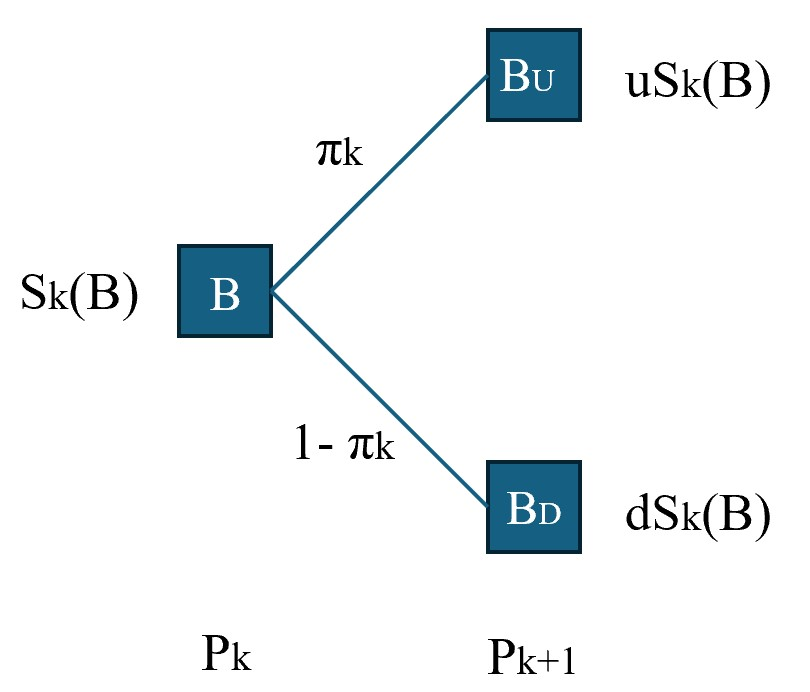
\includegraphics[width=7cm]{images/bin-mod-mart.jpg}
    \caption{Ausschnitt Zustandsbaum Binomialmodell}
    \label{fig:bin-mod-mart-prob}
\end{figure}
Abbildung \ref{fig:bin-mod-mart-prob} zeigt einen Zustandsbaum, wobei der Aktienkurs mit der Wahrscheinlichkeit im Martingalmass (\textit{Martingalwahrscheinlichkeit}) $\pi_k$ steigt und mit der Wahrscheinlichkeit $1-\pi_k$ fällt. Die Wahrscheinlichkeiten $\pi_k$ und $1-\pi_k$ lassen sich mithilfe derselben Methode wie in \ref{compute-mart-probs} berechnen:
$$\overline{uS_k}(B)\pi_k+\overline{dS_k}(B)(1-\pi_k)=\overline{S}_k(B)$$
und somit $$uS_k(B)\pi_k+dS_k(B)(1-\pi_k)=e^{r\Delta t}S_k(B)$$ und, wenn man durch $S_k(B)$ teilt,
$$u\pi_k+d(1-\pi_k)=e^{r\Delta t}$$ was sich zu $$\pi_k=\frac{e^{r\Delta t}-d}{u-d}$$ umformen lässt. Da die Wahrscheinlichkeiten gemäss den Voraussetzungen für alle $k$ gleich sind, ist allgemein $$\pi=\frac{e^{r\Delta t}-d}{u-d}$$
%\\Es muss $0<\pi_k<1$ und somit $$d<e^{r\Delta t}<u$$ gelten.
\subsection{Herleitung der Pricing-Formeln}
Für den Endzustand (bzw. Kurs der Anlage am Ende der Laufzeit) $\omega \in \Omega$ seien $N_U(\omega)$ resp. $N_D(\omega)$ die Anzahl Auf- resp. Abbewegungen, die nötig sind, um $\omega$ zu erreichen. 
\\Wie in Theorem \ref{th:init-pric-fct} erwähnt, ist $\mathcal{I}_0(X)=\mathcal{E}_\mathbb{P}(\overline{X})$. Im Fall des Binomialmodells ist also \label{binom-modell-allg-form}
\begin{align*}
    \mathcal{I}_0(X)&=\mathcal{E}(\overline{X})\\
    &=\mathcal{E}(Xe^{-rL})\\
    &=e^{-rL}\mathcal{E}(X)\\
    &=e^{-rL}\sum_{\omega \in \Omega}X(\omega)\mathbb{P}(\omega)\\
    &=e^{-rL}\sum_{\omega \in \Omega}X(\omega)\pi^{N_U(\omega)}(1-\pi)^{N_D(\omega)}
\end{align*}
Der Payoff einer Put-Option am Ende der Laufzeit ist $$X(\omega)=(K-S_T(\omega))^+=(K-S_0u^{N_U(\omega)}d^{N_D(\omega)})^+$$
Da $N_U(\omega)+N_D(\omega)=T$, kann man die Formel umschreiben zu
$$X(\omega)=(K-S_0u^{N_U(\omega)}d^{T-N_U(\omega)})^+$$
Die Entwicklung des Aktienkurses ist offensichtlich binomialverteilt, da der Kurs entweder steigen oder fallen kann, und somit lässt sich das vom Aktienkurs abhängige $\mathcal{I}_0(X)$ auch schreiben als
\begin{align*}
    \mathcal{I}_0(X)&=e^{-rL}\sum_{k=0}^{T}(K-S_0u^{k}d^{T-k})^+\binom{T}{k}\pi^k(1-\pi)^{T-k}\\
    &=e^{-rL}\sum_{k=0}^{T}\binom{T}{k}(K-S_0u^{k}d^{T-k})^+\pi^k(1-\pi)^{T-k}
\end{align*}
Dasselbe gilt für Call-Optionen, wobei dort für den Payoff $(S_0u^{k}d^{T-k}-K)^+$ statt $(K-S_0u^{k}d^{T-k})^+$ gilt. 

\begin{Theorem}{Binomialformeln}{binom-formulae}
    Es sei $\mathbb{M}$ ein vollständiges Binomialmodell mit keiner Arbitrage-Möglichkeit. Eine europäische Put-Option mit dem Ausübungspreis $K$ und der Laufzeit $L$, welche in $T$ Perioden eingeteilt wird, hat zum Zeitpunkt $t_0$ den Wert $$\mathcal{I}_0(\text{Put})=e^{-rL}\sum_{k=0}^{T}\binom{T}{k}(K-S_0u^{k}d^{T-k})^+\pi^k(1-\pi)^{T-k}$$
    Für Call-Optionen gilt $$\mathcal{I}_0(\text{Call})=e^{-rL}\sum_{k=0}^{T}\binom{T}{k}(S_0u^{k}d^{T-k}-K)^+\pi^k(1-\pi)^{T-k}$$ wobei $$\pi=\frac{e^{r\Delta t}-d}{u-d}$$ die Wahrscheinlichkeit im Martingalmass ist, dass der Kurs während einem Intervall steigt.
\end{Theorem}
\begin{Beispiel}{}{}
    Man will einen Call-Optionspreis berechnen. Eine Aktie hat momentan den Wert $\$120$. Der risikolose Zinssatz beträgt 5.3\%. Der Aktienkurs wird wahrscheinlich pro Monat um 2\% steigen oder um 2\% fallen. Die Laufzeit beträgt 3 Monate, der Ausübungspreis $\$110$. Die Wahrscheinlichkeit $\pi$ beträgt 
    $$\pi=\frac{e^{r\Delta t}-d}{u-d}=\frac{e^{0.053\cdot\frac{1}{12}}-0.98}{1.02-0.98}\approx0.61$$
    Somit ist 
    \begin{align*}
        \mathcal{I}_0&=e^{-0.053\cdot\frac{3}{12}}\sum_{k=0}^{3}\binom{3}{k}(120(1.02)^k(0.98)^{3-k}-110)^+(0.61)^k(0.39)^{3-k}\\
        &\approx0.986[1(2.943)^+\cdot0.0593+3(7.553)^+\cdot0.0927 +3(12.35)^+\cdot0.1451\\&+1(17.34)^+\cdot0.227]\\
        &\approx11.43
    \end{align*}
    Die oben beschriebene Call-Option würde also etwa $\$11.43$ kosten.
\end{Beispiel}
\subsection{Wahl der Parameter $r$, $d$ und $u$}
Um die oben hergeleiteten Formeln tatsächlich für echte Aktien verwenden zu können, muss man Zahlenwerte für $r$, $d$ und $u$ haben. Doch wie könnte man diese wählen?
\subsubsection{Risikoloser Zinssatz $r$}
Für den risikolosen Zinssatz $r$ werden oft die Zinssätze von Staatsanleihen genommen. Ein populäres Beispiel ist eine Anleihe des amerikanischen Finanzministeriums über drei Monate, der sogenannte \textit{U.S. 3 Month Treasury Bill}. Am 22. Juni 2024 verspricht dieser einen Zinssatz von 5.365\%.\footnote{https://www.cnbc.com/quotes/US3M (Abgerufen am 22. Juni 2024)}
\subsubsection{Faktoren $d$ und $u$}
Um einen Wert für $d$ bzw. $u$ zu erhalten, wird angenommen, dass sich die logarithmische Rendite $H_t$ folgendermassen entwickelt:
\begin{equation}\label{black-scholes-model}
    \ln{\frac{S_t}{S_0}}=H_t=\mu t + \sigma W_t
\end{equation}
$W_t$ ist eine Zufallsgrösse\label{brwn-motion}, wobei $W_0=0$, $W_{n+1}-W_n$ unabhängig von $W_{n}$ ist und $W_r-W_s$ (wobei $r>s$) normalverteilt mit Erwartungswert 0 und Varianz $r-s$ ist.\\Somit ist in Gleichung (\ref{black-scholes-model}) $W_t$ normalverteilt mit Erwartungswert 0 und Varianz $t-0=t$. Da $W_t$ normalverteilt ist, und $H_t$ linear von $W_t$ abhängt, ist auch $H_t$ normalverteilt. $H_t$ hat den Erwartungswert $\mu t$ und die Varianz $\sigma^2t$ und somit die Standardabweichung $\sigma \sqrt{t}$. Wenn man das Zeitintervall $[0, t]$ in viele kleinere Intervalle unterteilt und während diesen Intervallen jeweils die logarithmische Rendite $\ln{\frac{S_{i+\Delta t}}{S_i}}$ berechnet, ist das arithmetische Mittel $\mu \Delta t$ und die Standardabweichung $\sigma\sqrt{\Delta t}$.\\Da $H_t$ normalverteilt ist, beträgt die Wahrscheinlichkeit, dass ein Wert von $H_t$ ins Intervall $[\mu t -\sigma \sqrt{t}, \mu t + \sigma \sqrt{t}]$ fällt (das heisst, dass $H_t$ höchstens eine Standardabweichung vom Mittelwert entfernt ist), ca. 68\%. $d$ und $u$ können also als $$(d, u)=(e^{\mu t -\sigma \sqrt{t}}, e^{\mu t + \sigma \sqrt{t}})$$ definiert werden.\footnote{Man könnte $d$ und $u$ auch anders definieren. So zum Beispiel als $(d, u)=(e^{\mu t -3\sigma\sqrt{t}}, e^{\mu t + 3\sigma\sqrt{t}})$ da $H_t$ als normalverteilte Zufallsvariable mit einer Wahrscheinlichkeit von 99.7\% ins Intervall $[\mu t -3\sigma \sqrt{t}, \mu t + 3\sigma \sqrt{t}]$ fällt.} 
\begin{Beispiel}{}{u-d-derivation}
    Der Kurs einer Aktie betrug im ersten Monat \$120, im zweiten \$116, im dritten \$123, im vierten \$121 und im fünften \$127. Um später einen Optionspreis zu berechnen, wobei ein Intervall im Binomialmodell 30 Tage = $1$ Monat = $1/12$ Jahre lang ist, will man die Parameter $d$ und $u$ bestimmen. Es sind
    \begin{align*}
        \frac{1}{12}\mu  &= \frac{\ln{\frac{116}{120}}+\ln{\frac{123}{116}}+\ln{\frac{121}{123}}+\ln{\frac{127}{121}}}{4}\\
        &=\frac{-0.0339+0.0586-0.0164+0.0484}{4}\\
        &=0.0142
    \end{align*}
    und somit
    \begin{align*}
        \sqrt{\frac{1}{12}}\sigma&=\sqrt{\frac{(-0.0339-0.0142)^2+(0.0586-0.0142)^2+\ldots}{4}}\\
        &=0.0400
    \end{align*}
    Die Parameter $d$ und $u$ könnte man also berechnen als
    \begin{align*}
        d&=e^{0.0142-0.0400}=0.975\\
        u&=e^{0.0142+0.0400}=1.056
    \end{align*}
    \end{Beispiel}
\chapter{Amerikanische Optionen}
Im vorherigen Kapitel ging es um europäische Optionen. Europäische Optionen können erst am Ende der Laufzeit der Option ausgeübt werden. Eine ebenfalls beliebte Art von Optionen sind amerikanische Optionen. Diese können jederzeit von $t_0$ bis $t_T$ ausgeübt werden. Die Idee, welche im Folgenden verfolgt wird, ist, dass man sich eine Ausübungsstrategie $\tau$ vorstellt, welche festlegt, zu welchem Zeitpunkt man die Option ausüben soll, um das Beste rauszuholen.\\\\Für die Ausübungsstrategie $\tau$ gibt es eine Zufallsvariable $\mathbb{X}_\tau:\Omega\mapsto\mathbb{R}$, welche jedem Endzustand den entsprechenden Optionswert zuordnet. Wenn $\mathbb{X}_\tau$ erreichbar ist, kann man -- wie im vorherigen Kapitel bereits besprochen -- den Preis für $\mathbb{X}_\tau$ zur Zeit $t_0$ berechnen. Dieser Preis ist -- wie ebenso im vorherigen Kapitel bereits besprochen -- der erwartete abgezinste Wert $\mathcal{E}_\Pi(\overline{\mathbb{X}}_\tau)$, wobei $\Pi$ das Martingalmass ist. Das Ziel eines Investors ist also, eine Ausübungsstrategie $\tau$ zu finden, für die $\mathcal{E}_\Pi(\overline{\mathbb{X}}_\tau)$ maximal ist.
\section{Voraussetzungen}
Man stellt sich am einfachsten ein Modell mit diskreter Zeit $\mathbb{M}$ vor, welches die Informationsstruktur $$\mathbb{F}=(\mathcal{P}_0, \ldots, \mathcal{P}_T)$$ besitzt. Man nimmt an, dass dieses Modell keine Arbitrage-Möglichkeiten, das Martingalmass $\Pi$ und einen konstanten risikolosen Zinssatz $r$ besitzt. Man stellt sich eine amerikanische Option vor, welche zu jeder der Zeiten $$t_0< \ldots <t_T$$ ausgeübt werden kann.\\\\$Y_k$ sei der Wert der Option zum Zeitpunkt $t_k$, man nennt $\mathbb{Y}=(Y_0, \ldots, Y_T)$ den \textit{Payoff-Prozess}. $\mathbb{Y}$ sei $\mathbb{F}$-adaptiert. Man nimmt an, dass, wenn eine Option zum Zeitpunkt $t_k$ ausgeübt wird, der dabei erzielte Payoff noch bis $t_T$ mit dem risikolosen Zinssatz weiterwächst. Wenn man dies berücksichtigt, kann man $$X_k(\omega)=e^{r(t_T-t_k)}Y_k(\omega)$$ definieren, welche den Wert des Payoffs zum Zeitpunkt $t_T$ ausgibt. 
\section{Stoppzeiten}
Wenn man eine amerikanische Option besitzt, ist die Entscheidung sehr wichtig, wann man die Option ausübt. Es gebe also eine Zufallsvariable $\tau$, welche für jeden Endzustand $\omega$ bestimmt, zu welchem Zeitpunkt $t_k$ die Option im Fall, dass das Ereignis $\omega$ vorliegt, ausgeübt werden soll. Es gebe zudem eine Menge $\{\tau=k\}$, welche alle Endzustände $\omega$ beinhaltet, für welche die Option zum Zeitpunkt $t_k$ ausgeübt werden soll. $\{\tau=T\}$ soll alle $\omega$ beinhalten, für welche man die Option entweder zum Zeitpunkt $t_T$ ausüben oder einfach verfallen lassen soll. $\tau$ nennt man \textit{Stoppzeit}, $\{\tau=k\}$ nennt man \textit{Stoppereignis}.
\begin{Definition}{Stoppzeit und Stoppereignis}{stoptime-stopevent}
    Es sei $\mathcal{P}_k$ die Partition von $\Omega$ zum Zeitpunkt $t_k$. Die Zufallsvariable $\tau:\Omega\mapsto\{0, \ldots, T\}$ heisst \textit{Stoppzeit}, wobei das \textit{Stoppereignis}$$\{\tau=k\}=\{\omega\in\Omega|\tau(\omega)=k\}$$ $\mathcal{P}_k$-messbar ist. (Das heisst, dass $\{\tau=k\}$ entweder leer ist oder aus Blöcken von $\mathcal{P}_k$ besteht.) Die Zufallsvariable $\tau$ muss also $\mathbb{F}$-adaptiert sein, wobei $\mathbb{F}=(\mathcal{P}_0, \ldots, \mathcal{P}_T)$.\\Die Menge aller Stoppzeiten, welche zu einem der Zeitpunkte $t_k, \ldots, t_{k+j}$ stoppen, werde durch $\mathcal{S}_{k, k+j}$ symbolisiert. 
\end{Definition}
\begin{figure}[h]
    \centering
    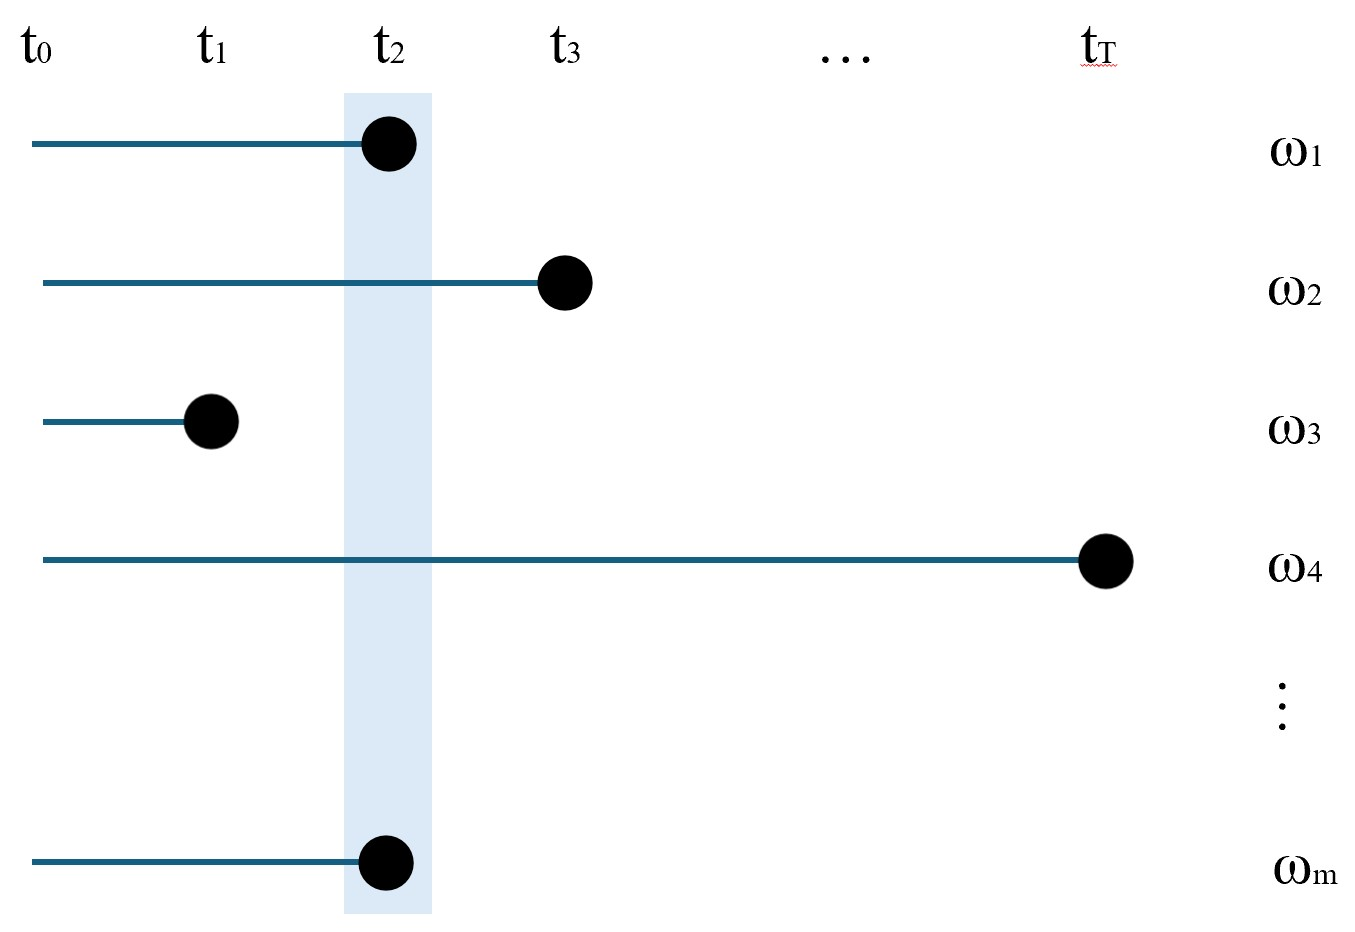
\includegraphics[width=12cm]{images/stoppzeit.jpg}
    \caption{Stoppzeit und Stoppereignis}
    \label{fig:stoppzeit}
\end{figure}
Abbildung \ref{fig:stoppzeit} visualisiert die unterschiedlichen Stoppzeiten für die Endzustände $\omega_k$ und das Stoppereignis $\{\tau=2\}$. Hierbei haben die Endzustände $\omega_1$ und $\omega_m$ die Stoppzeit $t_2$ und sind somit in $\{\tau=2\}$ enthalten. 
\subsection{Stoppzeiten zusammenfügen}
\begin{Theorem}{}{piecing-tg-stoptimes}
    Die Partition von $\Omega$ zum Zeitpunkt $t_k$ sei $\mathcal{P}_k=\{B_{k, 1}, \ldots, B_{k, c}\}$ und die Stoppzeiten $\tau_u\in\mathcal{S}_{k, T}$ für alle $u=1, \ldots, c$. Dann ist $$\tau^*=\sum_{u=1}^{c}\tau_u1_{B_{k, u}}$$auch eine Stoppzeit in $\mathcal{S}_{k, T}$.
\end{Theorem}
Dies lässt sich folgendermassen beweisen:
\begin{Beweis}{}{piecing-tg-stoptimes}
    Da laut Voraussetzung $\forall u:\tau_u\geq k$, ist auch $\tau^*\geq k$. Da $\mathcal{P}_k$ eine Partition von $\Omega$ ist, gilt für jedes beliebige $h\geq k$ $$\{\tau^*=h\}=\bigcup_{u=1}^{c}(\{\tau^*=h\}\cap B_{k, u})=\bigcup_{u=1}^{c}(\{\tau_u=h\}\cap B_{k, u})$$ Da $h\geq k$, ist $\mathcal{P}_h$ eine Verfeinerung von $\mathcal{P}_k$. $B_{k, u}$ und $\{\tau_u=h\}$ bestehen deshalb aus Blöcken von $\mathcal{P}_h$, dementsprechend besteht auch $\{\tau_u=h\}\cap B_{k, u}$ aus Blöcken von $\mathcal{P}_h$. Somit ist $\tau^*\in \mathcal{S}_{k, T}. $
\end{Beweis}
\section{Stoppzeiten und Payoff}
Die Zufallsvariable $\mathbb{X}_\tau$ gebe für jedes $\omega \in \Omega$ den Payoff, wenn die Stoppzeit $\tau$ berücksichtigt wird. Wenn $\mathbb{X}$ ein Payoff-Prozess ist, hat $\mathbb{X}_\tau$ zum Zeitpunkt $t_k$ den Preis 
\begin{equation}\label{eq:price-func-american}
    \mathcal{I}_k(\mathbb{X}_\tau)=\mathcal{E}_\Pi(e^{-r(t_T-t_k)}\mathbb{X}_\tau|\mathcal{P}_k)=e^{-r(t_T-t_k)}\mathcal{E}_\Pi(\mathbb{X}_\tau|\mathcal{P}_k)
\end{equation}
Um die bestmögliche Stoppzeit zu finden, muss man die Stoppzeit finden, für die $\mathcal{I}_k(\mathbb{X}_\tau)$ maximal wird und somit auch $\mathcal{E}_\Pi(\mathbb{X}_\tau|\mathcal{P}_k)$ maximal wird. 
\begin{Definition}{Optimaler Wert und Snell-Umhüllende}{optimal-value-snell-envelope}
    Es sei $\mathbb{X}=(X_0, \ldots, X_T)$ ein Payoff-Prozess. Es sei $\Pi$ ein Martingalmass für das Modell $\mathbb{M}$. Für jede Stoppzeit gebe $\mathbb{X}_\tau(\omega)$ den Payoff von $\mathbb{X}$ unter Berücksichtigung der Stoppzeit $\tau$. Der \textit{optimale Wert} von $\mathbb{X}$ für das Intervall $[k, T]$ sei $$\mathcal{M}_k(\mathbb{X})=\max\{\mathcal{E}_\Pi(\mathbb{X}_\tau|\mathcal{P}_k)|\tau \in \mathcal{S}_{k, T}\}$$Der optimale Wertprozess $\mathbb{S}=(\mathcal{M}_0(\mathbb{X}), \ldots, \mathcal{M}_T(\mathbb{X}))$ heisst \textit{Snell-Umhüllende} von $\mathbb{X}$. 
\end{Definition}
Da man, wie in der Einführung des Kapitels angetönt, den Payoff der Option maximieren will durch eine optimale Ausübungsstrategie, um den Wert einer amerikanischen Option zu berechnen, kann man $\mathbb{S}$ als den stochastischen Prozess betrachten, der die Entwicklung des Werts der Option über die Zeit darstellt. Um den Optionspreis zum Zeitpunkt $t_0$ zu berechnen, ist dementsprechend die Berechnung von $\mathcal{M}_0(\mathbb{X})$ das Endziel.
\begin{Definition}{Optimale Stoppzeit}{optimal-stoptime}
    Eine \textit{optimale Stoppzeit} von $\mathbb{X}$ im Intervall $[k, T]$ sei eine Stoppzeit $\tau^*$, für die gilt $$\mathcal{E}_\Pi(\mathbb{X}_{\tau^*}|\mathcal{P}_k)=\mathcal{M}_k(\mathbb{X})$$
\end{Definition}
Wichtig zu bemerken ist, dass die optimale Stoppzeit zum Zeitpunkt $t_k$ nur die Stoppzeit angibt, die zum Zeitpunkt $t_k$ wie die beste Stoppzeit wirkt auf Basis des momentanen Anlagewertes. Sie garantiert also nicht den allgemein bestmöglichen Payoff, weil man zum Zeitpunkt $t_k$ ja nicht in die Zukunft sehen kann und deshalb die optimale Stoppzeit -- salopp gesagt -- \textit{erraten} muss.
\section{Existenz von optimalen Stoppzeiten}
\begin{Theorem}{Existenz von optimalen Stoppzeiten}{exist-optimal-stoptimes}
    Für jedes Intervall $[k, T]$ existiert eine optimale Stoppzeit für $\mathbb{X}$. Wenn $$\mathcal{P}_k=\{B_{k, 1}, \ldots, B_{k, c}\}$$ die Partition von $\Omega$ zum Zeitpunkt $t_k$ ist und man für jedes $u$ eine Stoppzeit $\tau_u$ wählt, sodass $$\mathcal{E}_\Pi(\mathbb{X}_{\tau_u}|B_{k, u})=\max\{\mathcal{E}_\Pi(\mathbb{X}_\tau|B_{k, u})|\tau\in\mathcal{S}_{k, T}\}$$dann gilt für eine optimale Stoppzeit $\tau^*$ $$\tau^*=\sum_{u=1}^{c}\tau_u1_{B_{k, u}}$$
    Für alle $k$ ist somit $$\mathcal{E}_\Pi(\mathbb{X}_{\tau^*}|\mathcal{P}_k)=\mathcal{M}_k(\mathbb{X})$$
\end{Theorem}
\begin{Beweis}{Existenz von optimalen Stoppzeiten}{}
    Es sei $\mathcal{P}_k=\{B_{k, 1}, \ldots, B_{k, c}\}$ die Partition von $\Omega$ zum Zeitpunkt $t_k$. Wenn man die Stoppzeit optimieren will, maximiert man $$\mathcal{E}_\Pi(\mathbb{X}_\tau|\mathcal{P}_k)=\sum_{u=1}^{c}\mathcal{E}_\Pi(\mathbb{X}_\tau|B_{k, u})1_{B_{k, u}}$$Dieser Ausdruck ist nur maximal, wenn jedes $\mathcal{E}_\Pi(\mathbb{X}_\tau|B_{k, u})$ maximal ist für seinen Block $B_{k, u}$. Um $\mathcal{E}_\Pi(\mathbb{X}_\tau|\mathcal{P}_k)$ zu maximieren, wählt man also für jedes $u$ die Stoppzeit $\tau_u\in \mathcal{S}_{k, T}$, für die gilt $$\mathcal{E}_\Pi(\mathbb{X}_{\tau_u}|B_{k, u})\geq\mathcal{E}_\Pi(\mathbb{X}_\tau|B_{k, u})$$ für $\tau\in\mathcal{S}_{k, T}$. Wenn man die Stoppzeiten $\tau_u\in\mathcal{S}_{k, T}$ zu einer Stoppzeit $$\tau^*=\sum_{u=1}^{c}\tau_u1_{B_{k, u}}
$$ zusammenfasst, zeigt Theorem \ref{th:piecing-tg-stoptimes}, dass $\tau^*$ ebenfalls eine Stoppzeit in $\mathcal{S}_{k, T}$ ist. Somit ist für alle $\tau\in\mathcal{S}_{k, T}$ $$\mathcal{E}_\Pi(\mathbb{X}_{\tau^*}|\mathcal{P}_k)\geq\mathcal{E}_\Pi(\mathbb{X}_\tau|\mathcal{P}_k)$$ womit $\tau^*$ eine optimale Stoppzeit ist.
\end{Beweis}
\section{Snell-Umhüllende berechnen}
Angenommen, $\tau^*$ ist eine optimale Stoppzeit für $[k, T]$. Wenn $B$ ein Block in $\mathcal{P}_k$ ist, ist \begin{equation}\label{eq:snell-envelope-random}
    \mathcal{E}_\Pi(\mathbb{X}_{\tau^*}|B)=\max_{\tau\in\mathcal{S}_{k, T}}\{\mathcal{E}_\Pi(\mathbb{X}_\tau|B)\}=\frac{1}{\mathbb{P}(B)}\max_{\tau\in\mathcal{S}_{k, T}}\{\mathcal{E}_\Pi(\mathbb{X}_\tau1_B)\}
\end{equation} für $\tau\in\mathcal{S}_{k, T}$. Die optimale Stoppzeit ist also jene Stoppzeit, die den Erwartungswert $\mathcal{E}_\Pi(\mathbb{X}_\tau1_B)$ maximiert. Für jede Stoppzeit $\tau$ ist entweder $B\subseteq\{\tau=k\}$ oder $B\cap\{\tau=k\}=\emptyset$. Es ist also 
$$
\max_{\tau\in\mathcal{S}_{k, T}}\{\mathcal{E}_\Pi(\mathbb{X}_\tau 1_B)\} = \max \left\{ \max_{B\subseteq\{\tau = k\}} \{\mathcal{E}_\Pi(\mathbb{X}_\tau 1_B)\}, \max_{B \cap \{\tau = k\} = \emptyset, \tau \in \mathcal{S}_{k, T}} \{\mathcal{E}_\Pi(\mathbb{X}_\tau 1_B)\}\right\}
$$
Wenn $B\subseteq\{\tau=k\}$, ist $\mathbb{X}_\tau1_B$ einfach der Payoff $X_k1_B$, womit $$\max_{B\subseteq\{\tau=k\}}\{\mathcal{E}_\Pi(\mathbb{X}_\tau1_B)\}=X_k1_B$$
Um $\displaystyle \max_{B \cap \{\tau = k\} = \emptyset, \tau \in \mathcal{S}_{k, T}} \{\mathcal{E}_\Pi(\mathbb{X}_\tau 1_B)\}$ umzuschreiben, kann man sich überlegen, dass, wenn $B \cap \{\tau = k\} = \emptyset$, die Menge der möglichen Stoppzeiten für $\tau$ kleiner wird. Die Menge der Möglichkeiten für $\tau$ schrumpft also von $\mathcal{S}_{k, T}$ auf die kleinere Menge $\mathcal{S}_{k+1, T}$. Somit ist $$\max_{B \cap \{\tau = k\} = \emptyset, \tau \in \mathcal{S}_{k, T}} \{\mathcal{E}_\Pi(\mathbb{X}_\tau 1_B)\}=\max_{\tau\in\mathcal{S}_{k+1, T}}\{\mathcal{E}_\Pi(\mathbb{X}_\tau1_B)\}$$
womit gilt
$$\max_{\tau\in\mathcal{S}_{k, T}}\{\mathcal{E}_\Pi(\mathbb{X}_\tau 1_B)\}=\max\left\{\mathcal{E}(X_k1_B), \max_{\tau\in\mathcal{S}_{k+1, T}}\{\mathcal{E}_\Pi(\mathbb{X}_\tau1_B)\}\right\}$$
Dividiert man durch $\mathbb{P}(B)$, erhält man mithilfe der Gleichung \ref{eq:snell-envelope-random}
$$\mathcal{E}_\Pi(\mathbb{X}_{\tau^*}|B)=\max\left\{X_k(B), \max_{\tau\in\mathcal{S}_{k+1, T}}\{\mathcal{E}_\Pi(\mathbb{X}_\tau|B)\}\right\}$$
Dabei wurde $B$ als beliebiger Block von $\mathcal{P}_k$ definiert, womit -- ohne Beschränkung der Allgemeinheit und unter Berücksichtigung des Theorems \ref{th:exist-optimal-stoptimes}-- gilt, dass
$$\mathcal{M}_k(\mathbb{X})=\mathcal{E}_\Pi(\mathbb{X}_{\tau^*}|\mathcal{P}_k)=\max\left\{X_k, \max_{\tau\in\mathcal{S}_{k+1, T}}\{\mathcal{E}_\Pi(\mathbb{X}_\tau|\mathcal{P}_k)\}\right\}$$
Die Turmeigenschaft zeigt, dass
$$\mathcal{E}_\Pi(\mathbb{X}_\tau|\mathcal{P}_k)=\mathcal{E}_\Pi(\mathcal{E}_\Pi(\mathbb{X}_\tau|\mathcal{P}_{k+1})|\mathcal{P}_k)\leq\mathcal{E}_\Pi(\mathcal{M}_{k+1}(\mathbb{X})|\mathcal{P}_k)$$ für alle $\tau\in\mathcal{S}_{k+1, T}$, womit gilt
$$\max_{\tau\in\mathcal{S}_{k+1, T}}\{\mathcal{E}_\Pi(\mathbb{X}_\tau|\mathcal{P}_k)\}=\mathcal{E}_\Pi(\mathcal{M}_{k+1}(\mathbb{X})|\mathcal{P}_k)$$
Somit ist 
$$\mathcal{M}_k(\mathbb{X})=\max\left\{X_k, \mathcal{E}_\Pi(\mathcal{M}_{k+1}(\mathbb{X})|\mathcal{P}_k)\right\}$$
\begin{Beispiel}{}{am-option}
Abbildung \ref{fig:am-opt-statetree} zeigt ein Binomialmodell mit den Parametern $u=1.2, d=0.8, T=2, r=0$ und dem anfänglichen Anlagepreis $S_0=150$. $X$ steht für den Wert bzw. Payoff einer amerikanischen Call-Option mit Ausübungspreis $K=140$. Die Wahrscheinlichkeit im Martingalmass, dass der Kurs steigt, ist $$\pi=\frac{1-0.8}{1.2-0.8}=\frac{1}{2}$$ Man berechnet nun die Snell-Umhüllende:\\
Für $t_2$ ist $$\mathcal{M}_2(\mathbb{X})=X_2$$
Für $t_1$ ist $$\mathcal{E}(\mathcal{M}_2(\mathbb{X})|\mathcal{P}_1)=\mathcal{E}(X_2|\mathcal{P}_1)=\begin{cases}
    \frac{1}{2}(76+4)=40 &\text{falls } \omega\in B_{1, 1}\\
    \frac{1}{2}(4+0)=2 &\text{falls } \omega \in B_{1, 2}
\end{cases}$$
$$\mathcal{M}_1(\mathbb{X})=\max\{X_1, \mathcal{E}(\mathcal{M}_2(\mathbb{X})|\mathcal{P}_1)\}=\begin{cases}
    40 &\text{falls }\omega\in B_{1, 1}\\
    2 &\text{falls }\omega\in B_{1, 2}
\end{cases}$$
Für $t_0$ ist \begin{align*}
    \mathcal{M}_0(\mathbb{X})&=\max\{X_0, \mathcal{E}(\mathcal{M}_1(\mathbb{X})|\mathcal{P}_0)\}\\
    &=\max\{10, \frac{1}{2}(40+2)\}\\
    &=21
\end{align*}
Die oben beschriebene amerikanische Option würde also etwa \$21 kosten und man kann die Lücken in Abbildung \ref{fig:am-opt-statetree} ausfüllen (siehe Abbildung \ref{fig:am-opt-statetree-slvd}).
\end{Beispiel}
\begin{figure}[H]
    \centering
    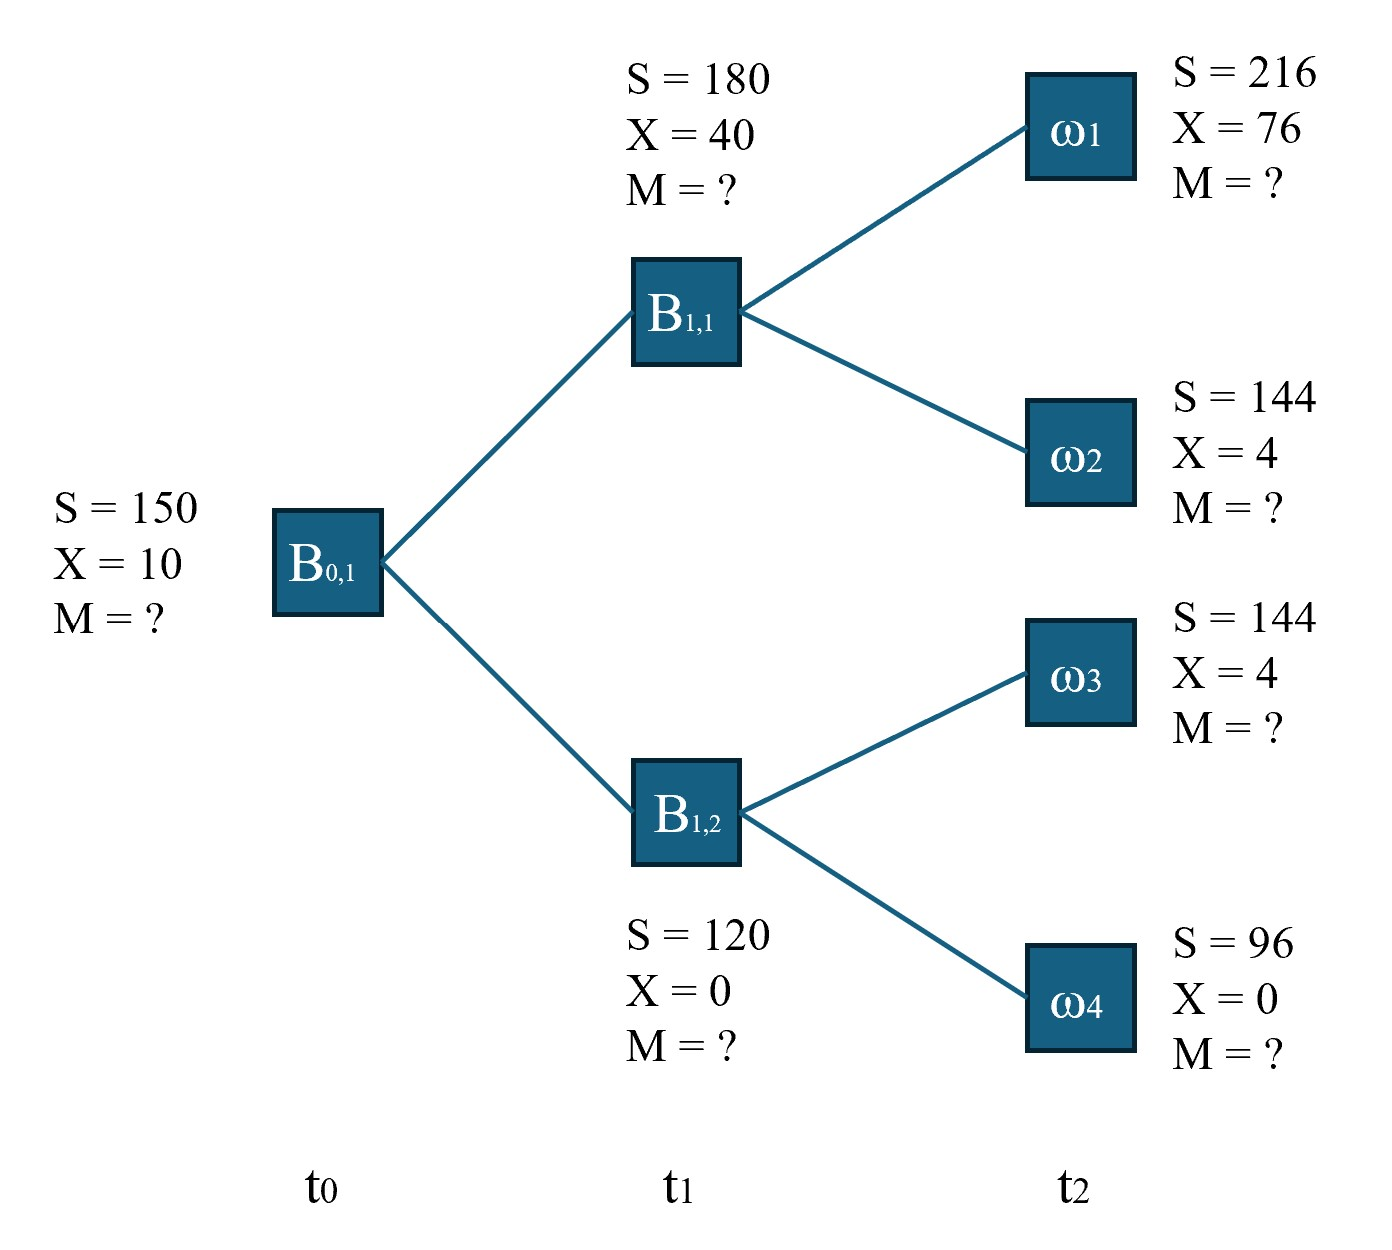
\includegraphics[width=9cm]{images/am-opt-statetree.jpg}
    \caption{Zustandsbaum im Binomialmodell}
    \label{fig:am-opt-statetree}
\end{figure}
\begin{figure}[H]
    \centering
    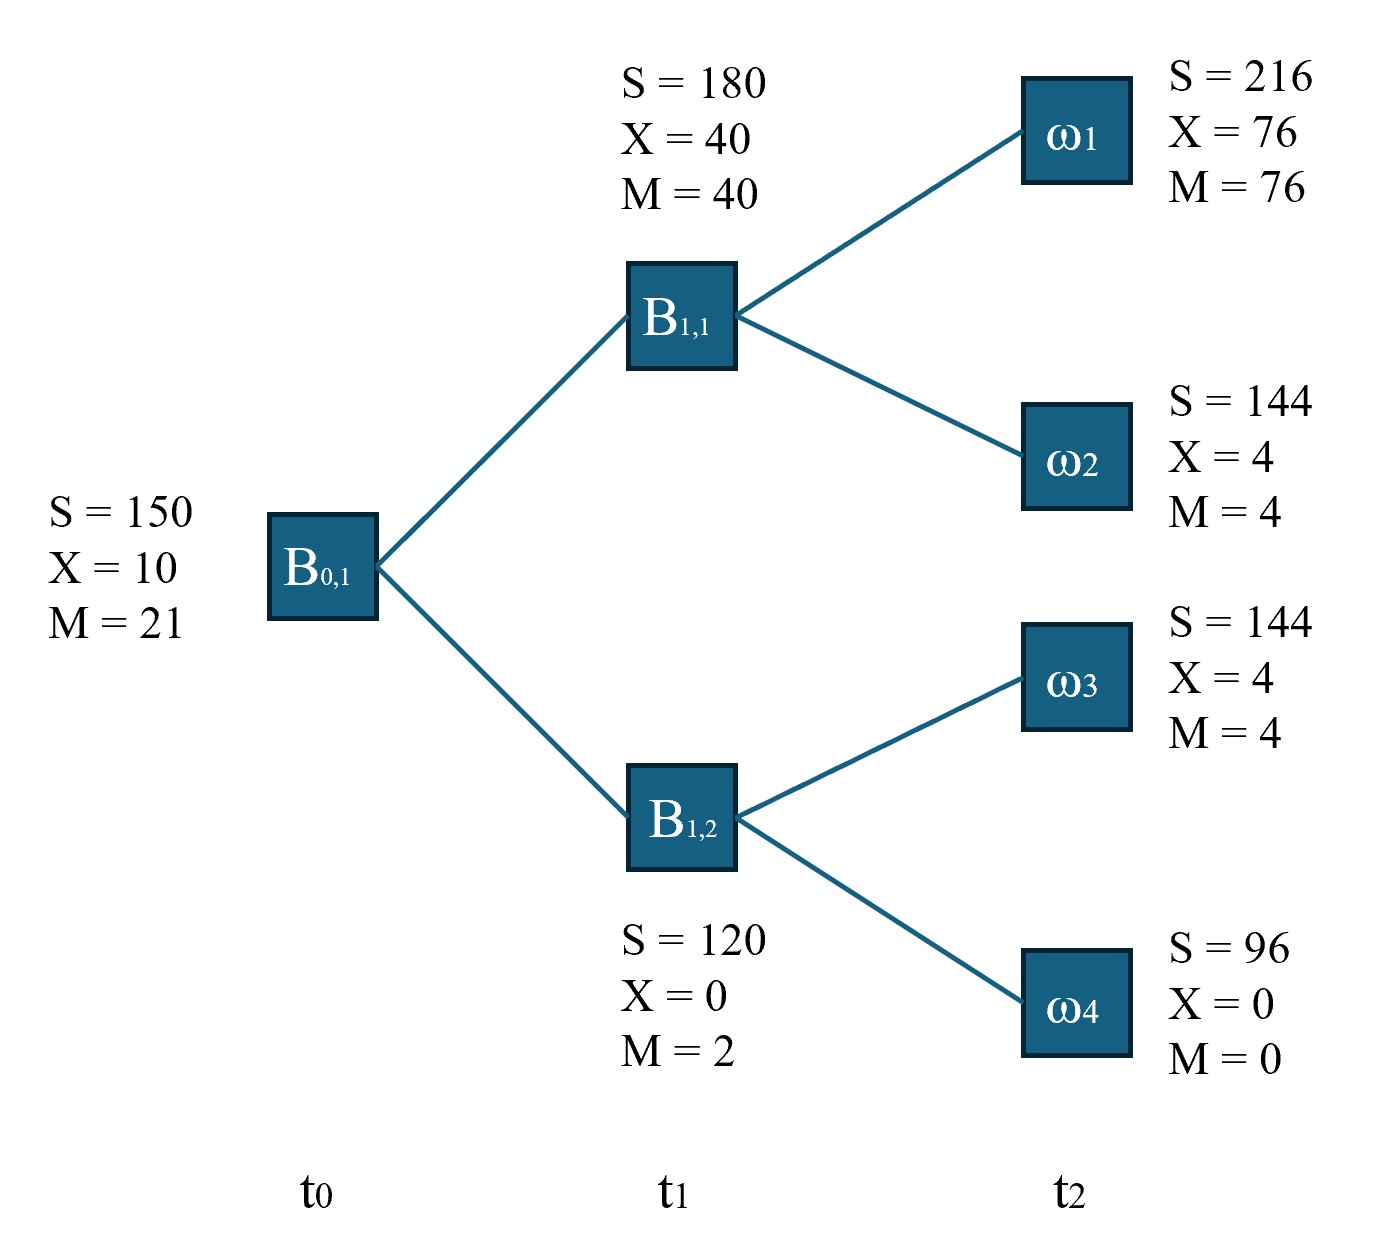
\includegraphics[width=9cm]{images/am-opt-statetree-slvd.jpg}
    \caption{Gelöster Zustandsbaum im Binomialmodell für $r=0$}
    \label{fig:am-opt-statetree-slvd}
\end{figure}
Jedoch ist in der Realität der risikolose Zinssatz meistens nicht 0. $X_k$ wurde als $$X_k(\omega)=e^{r(t_T-t_k)}Y_k(\omega)$$ definiert. In Gleichung \ref{eq:price-func-american} wurde deshalb das Preisfunktional definiert als $$\mathcal{I}_k(\mathbb{X}_\tau)=e^{-r(t_T-t_k)}\mathcal{E}_\Pi(\mathbb{X}_\tau|\mathcal{P}_k)$$ weil für $X_k$ der Payoff $Y_k$ jedes Mal auf den Zeitpunkt $t_T$ aufgezinst wird, damit man die Payoffs unterschiedlicher Zeitpunkte miteinander vergleichen kann. Wenn nun $r\neq0$, dann muss für die Berechnung von $\mathcal{M}_k(\mathbb{X})$ der erwartete Wert $\mathcal{E}(\mathcal{M}_{k+1}(\mathbb{X})|\mathcal{P}_k)$ zuerst abgezinst werden mit $e^{-r\Delta t}$. Man rechnet also effektiv \begin{equation*}
    \mathcal{M}_k(\mathbb{X})=\max\{X_k, e^{-r\Delta t}\mathcal{E}(\mathcal{M}_{k+1}(\mathbb{X})|\mathcal{P}_k)\}
\end{equation*} für $k<T$. Somit lässt sich die Option in Beispiel \ref{ex:am-option} jetzt auch für risikolose Zinssätze $r\neq0$ bepreisen.
\begin{Theorem}{Berechung der Snell-Umhüllenden}{calc-snell-envelope}
    Die Snell-Umhüllende lässt sich folgendermassen rekursiv berechnen:
    \\Für $r=0$:
    \begin{enumerate}
        \item $\mathcal{M}_T=X_T$
        \item $\mathcal{M}_k(\mathbb{X})=\max\left\{X_k, \mathcal{E}_\Pi(\mathcal{M}_{k+1}(\mathbb{X})|\mathcal{P}_k)\right\}$ für $k<T$
    \end{enumerate}
    Für $r\neq0$:
    \begin{enumerate}
        \item $\mathcal{M}_T=X_T$
        \item $\mathcal{M}_k(\mathbb{X})=\max\left\{X_k, e^{-r\Delta t}\mathcal{E}_\Pi(\mathcal{M}_{k+1}(\mathbb{X})|\mathcal{P}_k)\right\}$ für $k<T$
    \end{enumerate}
\end{Theorem}
\begin{Beispiel}{}{}
    Man betrachte dieselbe Option wie in Beispiel \ref{ex:am-option} bzw. Abbildung \ref{fig:am-opt-statetree}. Die Laufzeit des Modells sei $L=1$, womit $\Delta t = \frac{L}{T}=\frac{1}{2}$. Der risikolose Zinssatz sei $r=5.3\%$. Die Martingalwahrscheinlichkeit sei somit $$\pi=\frac{e^{0.053\cdot\frac{1}{2}}-0.8}{1.2-0.8}\approx0.57$$
    Somit ist für $t_2$ $$\mathcal{M}_2(\mathbb{X})=X_2$$
    Für $t_1$ ist \begin{align*}
        \mathcal{M}_1(\mathbb{X})&=\max\{X_1, e^{-r\Delta t}\mathcal{E}(\mathcal{M}_2(\mathbb{X})|\mathcal{P}_1)\}\\
        &=\begin{cases}
        \max\{40, e^{-0.053\cdot\frac{1}{2}}(76\pi+4(1-\pi))\}&\text{falls }\omega \in B_{1,1}\\
        \max\{0, e^{-0.053\cdot\frac{1}{2}}(4\pi+0(1-\pi))\}&\text{falls }\omega \in B_{1, 2}
        \end{cases}\\
        &\approx\begin{cases}
            \max\{40, 43.66\}&\text{falls }\omega\in B_{1,1}\\
            \max\{0, 2.21\}&\text{falls }\omega\in B_{1,2}
        \end{cases}\\
        &\approx\begin{cases}
            43.66&\text{falls }\omega\in B_{1,1}\\
            2.21&\text{falls }\omega\in B_{1,2}
        \end{cases}
    \end{align*}
    Für $t_0$ ist
    \begin{align*}
        \mathcal{M}_0(\mathbb{X})&=\max\{X_0, e^{-r\Delta t}\mathcal{E}(\mathcal{M}_1(\mathbb{X})|\mathcal{P}_0)\}\\
        &=\max\{10, e^{-0.053\cdot\frac{1}{2}}(43.66\pi+2.21(1-\pi))\}\\
        &=\max\{10, 25.04\}\\
        &=25.04
    \end{align*}
    Die Option würde also etwa \$25 kosten. Man kann nun den Zustandsbaum ausfüllen für den Fall, dass $r=5.3\%$ (siehe Abbildung \ref{fig:am-opt-statetree-slvd-r53}).
\end{Beispiel}
\begin{figure}[h]
    \centering
    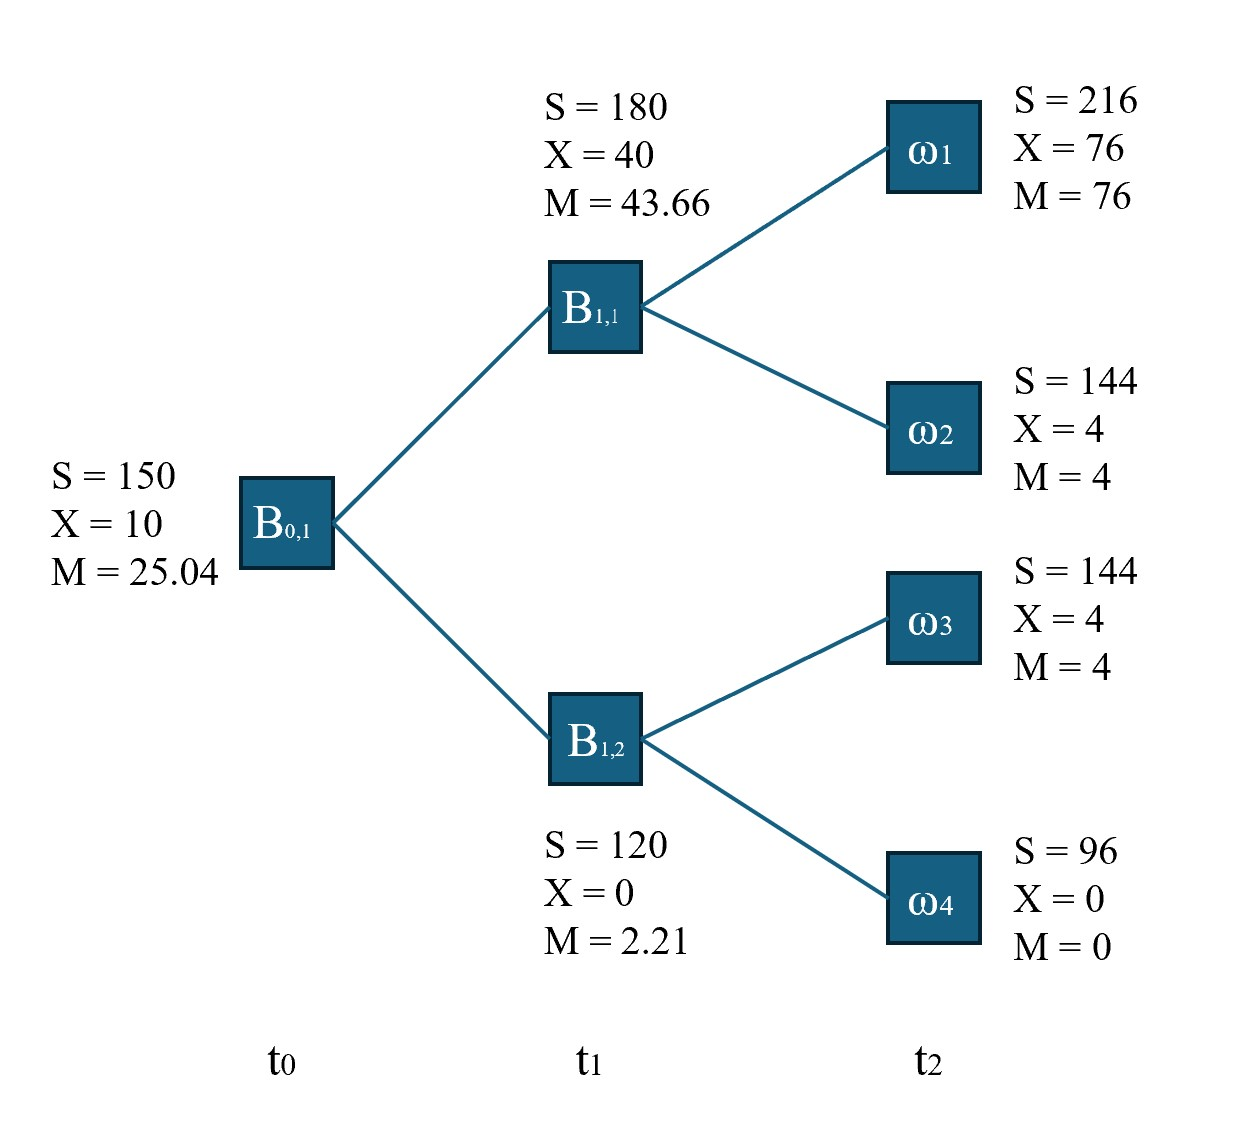
\includegraphics[width=9cm]{images/am-opt-statetree-slvd-r53.jpg}
    \caption{Gelöster Zustandsbaum im Binomialmodell für $r=5.3\%$}
    \label{fig:am-opt-statetree-slvd-r53}
\end{figure}

\chapter{Europäische Optionen -- Die Black-Scholes-Formeln}
In den vorherigen beiden Kapiteln wurde die Zeit in eine endliche Anzahl Schritte eingeteilt. Wenn man die Zeit jedoch als \textit{stetig} betrachtet, teilt man sie in \textit{unendlich} Schritte ein. Bei stetiger Zeit können sich Anlagepreise immer verändern und nicht mehr nur zu den endlichen vorgegebenen Zeitpunkten, wie es in den vorherigen Kapiteln der Fall war. Die Idee ist also, das Binomialmodell zu nehmen und zu schauen, was passiert, wenn die Schrittanzahl $T$ immer weiter wächst und schliesslich annähernd $\infty$ beträgt: $T \rightarrow \infty$.
\section{brownsche Bewegung}
Die brownsche Bewegung wurde bereits in \ref{brwn-motion} angetönt, dort jedoch nicht als solche bezeichnet.
\begin{Definition}{Stetiger stochastischer Prozess}{cont-stoch-process}
    Ein stetiger stochastischer Prozess über einem Intervall $I\subseteq \mathbb{R}$ ist die Menge $\{X_t|t\in I\}$ der Zufallsvariablen über $\Omega$. 
\end{Definition}
\begin{Definition}{brownsche Bewegung}{brownian-motion}
    Ein stetiger stochastischer Prozess $\mathcal{W}=\{W_t|t\geq0\}$ ist ein brownscher Bewegungsprozess mit Volatilität $\sigma$, wenn
    \begin{itemize}
        \item $W_0=0$
        \item alle $W_t-W_s$ normalverteilt mit Erwartungswert 0 und Varianz $\sigma^2(t-s)$ sind
        \item die Zuwächse $W_a-W_b$ und $W_b-W_c$ für $a\geq b \geq c$ unabhängig voneinander sind.
    \end{itemize}
    Wenn $\mu$ eine Konstante und $W_t$ ein brownscher Bewegungsprozess mit Volatilität $\sigma$ ist, nennt man $$\{\mu t + W_t|t\geq 0\}$$ \textit{brownsche Bewegung} mit \textit{Drift} $\mu$ und \textit{Volatilität} $\sigma$.\\\\
    Ein brownscher Bewegungsprozess $\{Z_t|t\geq 0\}$ mit Drift 0 und Volatilität 1 nennt man \textit{brownsche Standardbewegung}. $Z_t$ hat den Erwartungswert 0 und die Varianz $t$. Man kann einen beliebigen brownschen Bewegungsprozess $W_t$ mit Drift $\mu$ und Varianz $\sigma^2$ als $$W_t=\mu t + \sigma Z_t$$ darstellen.
\end{Definition}
\begin{figure}[H]
    \centering
    \begin{tikzpicture}
        \begin{axis}[title=brownsche Bewegung, xlabel=$t$,ylabel=$Z_t$, mark size = 0]
            \addplot+[
            scatter, 
            color=black % Set the color to black
            ]
            table[x index=0, y index=1]
            {brownian-motion.dat};
            \addplot+[
            scatter,
            color=red
            ]
            table[x index=0, y index=2]
            {brownian-motion.dat};
        \end{axis}
    \end{tikzpicture}
    \caption{Zwei Beispielpfade für brownsche Standardbewegung mit jeweils $365$ Schritten}
    \label{fig:brownian-motion}
\end{figure}

\subsection{Geometrische brownsche Bewegung}
In \ref{brwn-motion} wurde bereits die zeitliche Entwicklung von $$H_t=\ln{\frac{S_t}{S_0}}$$ als brownscher Bewegungsprozess betrachtet. Um die zeitliche Entwicklung des Aktienkurses $S_t=S_0e^{H_t}$ in Verbindung mit brownscher Bewegung zu setzen, definiert man den Prozess $\{e^{W_t}|t\geq0\}$ als \textit{geometrische brownsche Bewegung}, wobei $W_t$ ein brownscher Bewegungsprozess mit Drift $\mu$ und Volatilität $\sigma$ ist. Es gilt somit $$H_t=\mu t + \sigma W_t$$ womit $H_t$ normalverteilt ist mit Erwartungswert $\mu t$ und Varianz $\sigma^2t$. 
\begin{Theorem}{}{expected-val-variance-e-to-the-Y}
    Wenn $Y=\ln{X}$ normalverteilt\footnote{Man nennt $X$ auch \textit{logarithmisch normalverteilt}.} ist mit Erwartungswert $a$ und Varianz $b^2$, dann sind
    $$\mathcal{E}(X)=\mathcal{E}(e^Y)=e^{a+\frac{1}{2}b^2}$$
    $$\text{Var}(X)=\text{Var}(e^Y)=e^{2a+b^2}(e^{b^2}-1)$$
    Der Beweis findet sich im Anhang auf Seite \pageref{proof:lognorm-props}.
\end{Theorem}
Theorem \ref{th:expected-val-variance-e-to-the-Y} zeigt, dass
$$\mathcal{E}(S_t)=S_0e^{(\mu+\frac{1}{2}\sigma^2)t}$$
$$\text{Var}(S_t)=(S_0e^{(\mu+\frac{1}{2}\sigma^2)t})^2(e^{\sigma^2t}-1)$$
Wenn man $E_{k+1}=\frac{S_{k+1}}{S_k}$ als das Wachstum der Aktie während dem Zeitintervall $[t_k, t_{k+1}]$ definiert, ist $$S_T=S_0E_1\cdots E_T=S_0e^{\sum\ln{E_i}}$$ und somit
$$H_T=\sum_{i=1}^{T}\ln{E_i}$$
Man definiert nun wiederum die Werte $s_{k}$, für die gilt $$E_{k}=e^{s_{k}\Delta t} \Longleftrightarrow  s_{k}=\frac{1}{\Delta t}\ln{E_{k}}$$ Wenn $p$ bzw. $q=1-p$ die natürlichen\footnote{Das sind Wahrscheinlichkeiten, welche so wirklich in der \textit{echten Welt} vorkommen. Sie werden anhand von echten erhobenen Daten geschätzt. Sie sind nicht zwingend dieselben wie die Martingalwahrscheinlichkeiten, welche aufgrund von theoretischen Informationen berechnet werden.} Wahrscheinlichkeiten sind, für die der Aktienkurs steigt bzw. fällt, dann haben die Werte $s_k$\label{nat-drift-volat}
\begin{align*}
    \text{Erwartungswert } \mu&=\frac{1}{\Delta t}\mathcal{E}(\ln{E_i})=\frac{1}{\Delta t}(p\ln{u}+q\ln{d})\\
    \text{Varianz } s^2&=\frac{1}{(\Delta t)^2}\text{Var}(\ln{E_i})=\frac{1}{(\Delta t)^2}pq(\ln{u}-\ln{q})^2\\
\end{align*}
Der Ausdruck $$\sigma=s\sqrt{\Delta t}=\frac{1}{\sqrt{\Delta t}}\sqrt{pq}(\ln{u}-\ln{d})$$ heisst \textit{lokale Volatilität} des Aktienpreises.
Es gilt also
\begin{align*}
    \mathcal{E}(\ln{E_k})&=\mu\Delta t\\
    \text{Var}(\ln{E_k})&=\sigma^2\Delta t
\end{align*}
Somit kann man $\ln{E_k}$ standardisieren zu $$X_k=\frac{\ln{E_k}-\mu\Delta t}{\sigma\sqrt{\Delta t}}$$\label{vorheriger-abschnitt}
womit sich schreiben lässt, dass $$H_t=\sum_{i=1}^{T}\ln{E_i}=\sum_{i=1}^{T}(\sigma\sqrt{\Delta t}X_i+\mu\Delta t)=\mu L+\sigma\sqrt{\Delta t}\sum_{i=1}^{T}X_i$$ und somit $$S_t=S_0e^{H_t}=S_0e^{\mu L+\sigma\sqrt{\Delta t}\sum_{i=1}^{T}X_i}$$
Somit wird die Kursentwicklung der Aktie einerseits durch ein gleichmässiges Wachstum dank $\mu L$ und andererseits durch ein zufälliges Schwanken dank $\sigma\sqrt{\Delta t}\sum_{i=1}^{T}X_i$ bestimmt. Es sei $$\sigma\sqrt{\Delta t}\sum_{i=1}^{T}X_i=:Q_T$$ (Die Definition von $Q_T$ wird später gebraucht.) Da die Zufallsvariablen $X_i$ von den als konstant angenommenen Werten $p$, $d$ etc. abhängen und standardisiert sind, sind sie standardisierte Bernoulli-verteilte Zufallsvariablen, welche immer nur einen der beiden Werte $$X_i=\begin{cases}
    \frac{q}{\sqrt{pq}} \text{ mit Wahrscheinlichkeit $p$}\\
    \frac{-p}{\sqrt{pq}} \text{ mit Wahrscheinlichkeit $q$}
\end{cases}$$ annehmen können (der Beweis dazu findet sich im Anhang auf Seite \pageref{proof:bernoulli-dist-rand-var}). 
\section{Zentraler Grenzwertsatz}
\begin{Theorem}{Zentraler Grenzwertsatz}{central-limit-th}
Man stelle sich Zufallsvariablen vor, welche wie abgebildet in Dreiecksform angeordnet sind. 
    \begin{center}
    \begin{tabular}{ c c c c }
         $B_{1, 1}$ &  &  \\ 
         $B_{2, 1}$ & $B_{2, 2}$ & \\  
         $B_{3, 1}$ & $B_{3, 2}$ & $B_{3, 3}$\\
         $\vdots$ & $\vdots$ & $\vdots$ & $\ddots$
    \end{tabular}
\end{center}
In jeder Dreieckszeile $n$ seien die Zufallsvariablen $B_{n, i}$ unabhängige, identisch verteilte standardisierte Bernoulli-verteilte Zufallsvariablen. Es gilt für jede Zeile $n$
$$\mathbb{P}\left(B_{n, i}=\frac{q_n}{\sqrt{p_nq_n}}\right)=p_n, \mathbb{P}\left(B_{n, i}=\frac{-p_n}{\sqrt{p_nq_n}}\right)=q_n$$Wenn die Wahrscheinlichkeiten $p_n$ für steigende $n$ gegen $p$ konvergieren, nähert sich die Verteilung der Zufallsvariablen $$S_n=\frac{1}{\sqrt{n}}\sum_{i=1}^{n}B_{n, i}$$ einer Standardnormalverteilung.
Man schreibt $$S_n\xrightarrow{dist}Z$$ wobei $Z$ eine standardnormalverteilte Zufallsvariable ist.\\\\(Der zentrale Grenzwertsatz kann auch anders formuliert werden und wird im Rahmen dieser Arbeit nicht bewiesen.)
\end{Theorem}
Der zentrale Grenzwertsatz wird nun auch auf die Situation im Abschnitt \ref{vorheriger-abschnitt} angewendet. Die Zufallsvariablen $X_i$ werden in Dreiecksform angeordnet. Jede Zeile $k$ im Dreieck steht für ein Binomialmodell mit $T=k$:
    \begin{center}
    \begin{tabular}{ c c c c c }
         $\mathbb{M}_1$: & $X_{1, 1}$ &  &  \\ 
         $\mathbb{M}_2$: & $X_{2, 1}$ & $X_{2, 2}$ & \\  
         $\mathbb{M}_3$: & $X_{3, 1}$ & $X_{3, 2}$ & $X_{3, 3}$\\
         &$\vdots$ & $\vdots$ & $\vdots$ & $\ddots$
    \end{tabular}
\end{center}
Jedes Modell $\mathbb{M}_k$ hat den Wahrscheinlichkeitsraum $(\Omega_T, \mathbb{P}_T)$ und es gilt für jedes Modell $\mathbb{M}_k$ bzw. Zeile $k$, dass $$\mathbb{P}_T\left(X_{T, i}=\frac{1-p_T}{\sqrt{p_T(1-p_T)}}\right)=p_T,\ \mathbb{P}_T\left(X_{T, i}=\frac{-p_T}{\sqrt{p_T(1-p_T)}}\right)=1-p_T$$
Angenommen, $p_T\rightarrow p$, dann sagt der Satz, dass die Verteilung von $$\frac{1}{\sqrt{T}}\sum_{i=1}^{T}X_{T, i}=\frac{1}{\sigma_T\sqrt{t}}Q_T$$ für steigende $T$ gegen eine standardnormalverteilte Zufallsvariable konvergiert: $$\frac{1}{\sigma_T\sqrt{t}}Q_T\xrightarrow{dist}Z_T$$ womit ebenfalls
\begin{align*}
    Q_T&\xrightarrow{dist}\sigma_T\sqrt{t}Z_T\\
    \mu_Tt+Q_T=H_T&\xrightarrow{dist}\mu_Tt+\sigma_T\sqrt{t}Z_T=H_T
\end{align*}
womit $$S_T\xrightarrow{dist}S_0e^{H_t}=S_0e^{\mu t+\sigma\sqrt{t}Z_t}$$
\section{Natürliche Wahrscheinlichkeit und Martingalwahrscheinlichkeit}
Der Payoff einer europäischen Call-Option mit Ausübungspreis $K$ ist $$X=(S_T-K)^+=(S_0e^{H_T}-K)^+$$ Wie früher bereits mehrmals verwendet, ist der Anfangspreis der Call-Option (wenn $t$ die Laufzeit des Modells ist) $$\mathcal{I}(\text{Call})=e^{-rt}\mathcal{E}_\mathbb{P}((S_0e^{H_T}-K)^+)$$ wobei der Erwartungswert mithilfe des Martingalmasses $\mathbb{P}$ bestimmt wird. Vergrössert man die Anzahl Schritte im Modell unendlich oft, erhält man den Call-Preis $C_\infty$:
$$C_\infty=\lim_{T\to\infty}\mathcal{I}(\text{Call})=e^{-rt}\lim_{T\to\infty}\mathcal{E}((S_0e^{H_T}-K)^+)$$
Die Werte $S_0$, $e$ und $K$ verändern sich für steigende $T$ nicht, weshalb man nun den Wert zu finden probiert, dem sich $H_T$ für steigende $T$ annähert.
\subsection{Wahrscheinlichkeiten}
Es sei $p$ die natürliche Wahrscheinlichkeit, dass der Kurs steigt. In \ref{nat-drift-volat} wurden die Gleichungen für $\mu$ und die lokale Volatilität $\sigma$ hergeleitet. Ausgedrückt mit der natürlichen Wahrscheinlichkeit $p$, erhält man die \textit{natürliche Drift} $$\mu=\frac{1}{\Delta t}(p\ln{u_T}+(1-p)\ln{d_T})$$ und die \textit{natürliche Volatilität} $$\sigma^2=\frac{1}{\Delta t}p(1-p)(\ln{u_T}-\ln{d_T})^2$$Um zu sehen, was mit der Martingalwahrscheinlichkeit $\pi_T$ für steigende $T$ passiert, löst man $\mu$ und $\sigma$ auf $\ln{u_T}$ und $\ln{d_T}$ auf, was die Lösungen
\begin{align*}
    \ln{u_T}&=\mu\Delta t +\sigma\sqrt{\Delta t}\frac{1-p}{\sqrt{p(1-p)}}\\
    \ln{d_T}&=\mu\Delta t - \sigma\sqrt{\Delta t}\frac{p}{\sqrt{p(1-p)}}
\end{align*}
hat, womit
\begin{align*}
    u_T&=e^{\mu\Delta t +\sigma\sqrt{\Delta t}\frac{1-p}{\sqrt{p(1-p)}}}\\
    d_T&=e^{\mu\Delta t - \sigma\sqrt{\Delta t}\frac{p}{\sqrt{p(1-p)}}}
\end{align*}
Somit ist die Martingalwahrscheinlichkeit
\begin{align*}
    \pi_T&=\frac{e^{r\Delta t}-d_T}{u_T-d_T}\\
    &=\frac{e^{r\Delta t}-e^{\mu\Delta t - \sigma\sqrt{\Delta t}\frac{p}{\sqrt{p(1-p)}}}}{e^{\mu\Delta t +\sigma\sqrt{\Delta t}\frac{1-p}{\sqrt{p(1-p)}}}-e^{\mu\Delta t - \sigma\sqrt{\Delta t}\frac{p}{\sqrt{p(1-p)}}}}\\
    &=\frac{e^{(r-\mu)\Delta t}-e^{-\sigma\sqrt{\Delta t}\frac{p}{\sqrt{p(1-p)}}}}{e^{\sigma\sqrt{\Delta t}\frac{1-p}{\sqrt{p(1-p)}}}-e^{-\sigma\sqrt{\Delta t}\frac{p}{\sqrt{p(1-p)}}}}\\
    &=\frac{e^{(r-\mu)\Delta t+\frac{p}{\sqrt{p(1-p)}}\sigma\sqrt{\Delta t}}-1}{e^{\frac{1}{\sqrt{p(1-p)}}\sigma\sqrt{\Delta t}}-1}
\end{align*}
Es  wird nun mithilfe der Regel von de l'Hôpital\footnote{Mehr zur Regel von de l'Hôpital findet sich im Anhang auf Seite \pageref{th:delhopital-rule}.} für $T\rightarrow\infty$ bzw. $\Delta t \rightarrow 0$ der Grenzwert berechnet:
\begin{align*}
    \lim_{T \to \infty}\pi_T&=\lim_{\Delta t \to 0}\frac{e^{(r-\mu)\Delta t+\frac{p}{\sqrt{p(1-p)}}\sigma\sqrt{\Delta t}}-1}{e^{\frac{1}{\sqrt{p(1-p)}}\sigma\sqrt{\Delta t}}-1}\\
    &=\lim_{\Delta t \to 0}\frac{(r-\mu+\frac{p\sigma}{\sqrt{p(1-p)}}\frac{1}{2\sqrt{\Delta t}})e^{(r-\mu)\Delta t+\frac{p}{\sqrt{p(1-p)}}\sigma\sqrt{\Delta t}}}{(\frac{\sigma}{\sqrt{p(1-p)}}\frac{1}{2\sqrt{\Delta t}})e^{\frac{1}{\sqrt{p(1-p)}}\sigma\sqrt{\Delta t}}}\\
    &=\lim_{\Delta t \to 0}\left(\frac{r-\mu+\frac{p\sigma}{\sqrt{p(1-p)}}\frac{1}{2\sqrt{\Delta t}}}{\frac{\sigma}{\sqrt{p(1-p)}}\frac{1}{2\sqrt{\Delta t}}}\frac{e^{(r-\mu)\Delta t+\frac{p}{\sqrt{p(1-p)}}\sigma\sqrt{\Delta t}}}{e^{\frac{1}{\sqrt{p(1-p)}}\sigma\sqrt{\Delta t}}}\right)\\
    &=\lim_{\Delta t \to 0}\left(\frac{r-\mu+\frac{p\sigma}{\sqrt{p(1-p)}}\frac{1}{2\sqrt{\Delta t}}}{\frac{\sigma}{\sqrt{p(1-p)}}\frac{1}{2\sqrt{\Delta t}}}\right)\frac{e^0}{e^0}\\
    &=\lim_{\Delta t \to 0}\left(\frac{r-\mu}{\frac{\sigma}{\sqrt{p(1-p)}}\frac{1}{2\sqrt{\Delta t}}}+\frac{p\left(\frac{\sigma}{\sqrt{p(1-p)}}\frac{1}{2\sqrt{\Delta t}}\right)}{\frac{\sigma}{\sqrt{p(1-p)}}\frac{1}{2\sqrt{\Delta t}}}\right)\\
    &=\lim_{\Delta t \to 0}\left(\frac{r-\mu}{\frac{\sigma}{\sqrt{p(1-p)}}}2\sqrt{\Delta t}\right)+p\\
    &=0+p\\
    &=p
\end{align*}
Erhöht man die Schrittanzahl $T$, so nähert sich also die Wahrscheinlichkeit im Martingalmass $\pi_T$ der natürlichen Wahrscheinlichkeit $p$.
\subsection{Drift und Volatilität}
Man stelle sich die (im Dreieck angeordneten) Binomialmodelle $\mathbb{M}_{\pi, T}$ vor, wie sie früher bereits behandelt wurden. Sie haben die Martingalwahrscheinlichkeiten $\pi_T$ dafür, dass der Aktienkurs steigt. Wie verhalten sich nun Drift $$\mu_{\pi, T}=\frac{1}{\Delta t}(\pi_T\ln{u_T}+(1-\pi_T)\ln{d_T})$$ und Volatilität $$\sigma_{\pi, T}=\frac{1}{\sqrt{\Delta t}}\sqrt{\pi_T(1-\pi_T)}(\ln{u_T}-\ln{d_T})$$ im Grenzwert $T\to\infty$? In welcher Beziehung stehen sie zu der \textit{natürlichen} Drift $\mu_p$ bzw. der \textit{natürlichen} Volatilität $\sigma_p$?
\\Es gilt
\begin{align*}
    \mu_{\pi, T}&=\frac{1}{\Delta t}(\pi_T\ln{u}+(1-\pi_T)\ln{d})\\
    \mu_p&=\frac{1}{\Delta t}(p\ln{u}+(1-p)\ln{d})
\end{align*}
womit $$\mu_{\pi, T}-\mu_p=\frac{1}{\Delta t}(\pi_T-p)(\ln{u}-\ln{d})$$
gilt. Zudem ist $$\sigma_p=\frac{1}{\sqrt{\Delta t}}\sqrt{p(1-p)}(\ln{u}-\ln{d})$$
womit wiederum 
\begin{align*}
    \frac{\mu_{\pi, T}-\mu_p}{\sigma_p}&=\frac{1}{\sqrt{\Delta t}}\frac{\pi_T-p}{\sqrt{p(1-p)}}\\
    \mu_{\pi, T}&=\sigma_p\frac{1}{\sqrt{\Delta t}}\frac{\pi_T-p}{\sqrt{p(1-p)}}+\mu_p
\end{align*}
Und, wenn $T\rightarrow\infty$ bzw. $\Delta t \to 0$,
$$\lim_{T\to\infty}\mu_{\pi, T}=\frac{\sigma_p}{\sqrt{p(1-p)}}\lim_{\Delta t \to 0}\left(\frac{\pi_T-p}{\sqrt{\Delta t}}\right)+\mu_p$$
Für den Grenzwert auf der rechten Seite gilt 
\begin{align*}
    \lim_{\Delta t \to 0}\left(\frac{\pi_T-p}{\sqrt{\Delta t}}\right)&=\lim_{\Delta t \to 0}\frac{1}{\sqrt{\Delta t}}(\pi_T-p)\\
    &=\lim_{\Delta t \to 0}\frac{1}{\sqrt{\Delta t}}\left(\frac{e^{(r-\mu_p)\Delta t+\frac{p}{\sqrt{p(1-p)}}\sigma_p\sqrt{\Delta t}}-1}{e^{\frac{1}{\sqrt{p(1-p)}}\sigma_p\sqrt{\Delta t}}-1}-p\right)
\end{align*}
Diesen Grenzwert berechnet man nun:
\begin{align*}
    \lim_{\Delta t \to 0}\frac{1}{\sqrt{\Delta t}}\left(\frac{e^{(r-\mu_p)\Delta t+\frac{p}{\sqrt{p(1-p)}}\sigma_p\sqrt{\Delta t}}-1}{e^{\frac{1}{\sqrt{p(1-p)}}\sigma_p\sqrt{\Delta t}}-1}-p\right)\\
    &=\lim_{\Delta t \to 0}\frac{e^{(r-\mu_p)\Delta t+\frac{p}{\sqrt{p(1-p)}}\sigma_p\sqrt{\Delta t}}-1-pe^{\frac{1}{\sqrt{p(1-p)}}\sigma_p\sqrt{t}}+p}{\sqrt{\Delta t}e^{\frac{1}{\sqrt{p(1-p)}}\sigma_p\sqrt{\Delta t}}-\sqrt{\Delta t}}
\end{align*}
Mithilfe der Regel von de l'Hôpital erhält man
\begin{align*}
    &\lim_{\Delta t \to 0}\frac{\left(r-\mu_p+\frac{p\sigma_p}{\sqrt{p(1-p)}}\frac{1}{2\sqrt{\Delta t}}\right)e^{(r-\mu_p)\Delta t+\frac{p}{\sqrt{p(1-p)}}\sigma_p\sqrt{\Delta t}}-p\frac{\sigma_p}{\sqrt{p(1-p)}}\frac{1}{2\sqrt{\Delta t}}e^{\frac{1}{\sqrt{p(1-p)}}\sigma_p\sqrt{\Delta t}}}{\frac{1}{2\sqrt{\Delta t}}e^{\frac{1}{\sqrt{p(1-p)}}\sigma_p\sqrt{\Delta t}}+\sqrt{\Delta t}\frac{\sigma_p}{\sqrt{p(1-p)}}\frac{1}{2\sqrt{\Delta t}}e^{\frac{1}{\sqrt{p(1-p)}}\sigma_p\sqrt{\Delta t}}-\frac{1}{2\sqrt{\Delta t}}}\\
    &=\lim_{\Delta t \to 0}\frac{\left(2\sqrt{\Delta t}(r-\mu_p)+\frac{p\sigma_p}{\sqrt{p(1-p)}}\right)e^{(r-\mu_p)\Delta t+\frac{p}{\sqrt{p(1-p)}}\sigma_p\sqrt{\Delta t}}-p\frac{\sigma_p}{\sqrt{p(1-p)}}e^{\frac{1}{\sqrt{p(1-p)}}\sigma_p\sqrt{\Delta t}}}{e^{\frac{1}{\sqrt{p(1-p)}}\sigma_p\sqrt{\Delta t}}+\sqrt{\Delta t}\frac{\sigma_p}{\sqrt{p(1-p)}}e^{\frac{1}{\sqrt{p(1-p)}}\sigma_p\sqrt{\Delta t}}-1}
\end{align*}
Um Platz zu sparen, wird $$n=(r-\mu_p)\Delta t+\frac{p}{\sqrt{p(1-p)}}\sigma_p\sqrt{\Delta t}$$ gesetzt, wobei gilt, dass $$\lim_{\Delta t \to 0}n = 0\ \text{und}\ \lim_{\Delta t \to 0}e^n = 1$$Nun wendet man die Regel von de l'Hôpital ein zweites Mal an:
\begin{align*}
    &\lim_{\Delta t \to 0}\frac{\frac{2(r-\mu_p)}{2\sqrt{\Delta t}}e^{n}+\left(2\sqrt{\Delta t}(r-\mu_p)+\frac{p\sigma_p}{\sqrt{p(1-p)}}\right)\left((r-\mu_p)+\frac{p\sigma_p}{\sqrt{p(1-p)}}\frac{1}{2\sqrt{\Delta t}}\right)e^{n}\linebreak-\frac{p\sigma_p^2}{p(1-p)}\frac{1}{2\sqrt{\Delta t}}e^{\frac{\sigma_p\sqrt{\Delta t}}{\sqrt{p(1-p)}}}}{\frac{\sigma_p}{\sqrt{p(1-p)}}\frac{1}{2\sqrt{\Delta t}}e^{\frac{1}{\sqrt{p(1-p)}}\sigma_p\sqrt{\Delta t}}+\frac{1}{2\sqrt{\Delta t}}\frac{\sigma_p}{\sqrt{p(1-p)}}e^{\frac{1}{\sqrt{p(1-p)}}\sigma_p\sqrt{\Delta t}}+\sqrt{\Delta t}\frac{\sigma_p^2}{p(1-p)}\frac{1}{2\sqrt{\Delta t}}e^{\frac{1}{\sqrt{p(1-p)}}\sigma_p\sqrt{\Delta t}}}\\
    &=\lim_{\Delta t \to 0}\frac{2(r-\mu_p)e^n+2\sqrt{\Delta t}\left( 2\sqrt{\Delta t}(r-\mu_p)^2+2(r-\mu_p)\frac{p\sigma_p}{\sqrt{p(1-p)}}+\frac{1}{2\sqrt{\Delta t}}\frac{p^2\sigma_p^2}{p(1-p)} \right)e^{n}-\frac{p\sigma^2}{p(1-p)}e^{\frac{\sigma_p\sqrt{\Delta t}}{\sqrt{p(1-p)}}}}{\frac{2\sigma_p}{\sqrt{p(1-p)}}e^{\frac{\sigma_p\sqrt{\Delta t}}{\sqrt{p(1-p)}}}+\sqrt{\Delta t}\frac{\sigma_p^2}{p(1-p)}e^{\frac{\sigma_p\sqrt{\Delta t}}{\sqrt{p(1-p)}}}}\\
    &=\lim_{\Delta t \to 0}\frac{2(r-\mu_p)e^n+\left( 4\Delta t(r-\mu_p)^2+4\sqrt{\Delta t}(r-\mu_p)\frac{p\sigma_p}{\sqrt{p(1-p)}}+\frac{p^2\sigma_p^2}{p(1-p)} \right)e^{n}-\frac{p\sigma^2}{p(1-p)}e^{\frac{\sigma_p\sqrt{\Delta t}}{\sqrt{p(1-p)}}}}{\frac{2\sigma_p}{\sqrt{p(1-p)}}e^{\frac{\sigma_p\sqrt{\Delta t}}{\sqrt{p(1-p)}}}+\sqrt{\Delta t}\frac{\sigma_p^2}{p(1-p)}e^{\frac{\sigma_p\sqrt{\Delta t}}{\sqrt{p(1-p)}}}}\\
    &=\frac{2(r-\mu_p)+\frac{p^2\sigma_p^2}{p(1-p)}-\frac{p\sigma_p^2}{p(1-p)}}{\frac{2\sigma_p}{\sqrt{p(1-p)}}}\\
    &=\frac{2(r-\mu_p)+\frac{p\sigma_p^2}{1-p}-\frac{\sigma_p^2}{1-p}}{\frac{2\sigma_p}{\sqrt{p(1-p)}}}\\
    &=\frac{2(r-\mu_p)+\sigma_p^2\left(\frac{p}{1-p}-\frac{1}{1-p}\right)}{2\sigma_p}\sqrt{p(1-p)}\\
    &=\frac{2(r-\mu_p)-\sigma_p^2}{2\sigma_p}\sqrt{p(1-p)}
\end{align*}
Somit ist
\begin{align*}
    \lim_{T\to\infty}\mu_{\pi, T}&=\frac{\sigma_p}{\sqrt{p(1-p)}}\left(\frac{2(r-\mu_p)-\sigma_p^2}{2\sigma_p}\sqrt{p(1-p)}\right)+\mu_p\\
    &=\frac{2(r-\mu_p)-\sigma_p^2}{2}+\mu_p\\
    &=r-\mu_p-\frac{\sigma_p^2}{2}+\mu_p\\
    &=r-\frac{\sigma_p^2}{2}
\end{align*}
Für die Volatilitäten gilt
\begin{align*}
    \sigma_{\pi, T}^2&=\frac{1}{\Delta t}(\pi_T(1-\pi_T))(\ln{u}-\ln{d})^2\\
    \sigma_p^2&=\frac{1}{\Delta t}(p(1-p))(\ln{u}-\ln{d})^2
\end{align*}
womit $$\frac{\sigma_{\pi, T}^2}{\sigma_p^2}=\frac{\pi_T(1-\pi_T)}{p(1-p)}$$
Weil aber, wie oben gezeigt, $\pi_T\rightarrow p$ für steigende $T$, ist
$$\lim_{T\to\infty}\frac{\sigma_{\pi, T}^2}{\sigma_p^2}=1$$
womit $$\lim_{T\to\infty}\sigma_{\pi, T}=\sigma_p$$
\begin{Theorem}{}{relation-mart-nat-prob}
    Es sei $\mathbb{M}_{t, T}$ ein Binomialmodell mit Martingalmass, wobei es
    \begin{itemize}
        \item die Laufzeit $t\geq0$
        \item $T=\frac{t}{\Delta t}$ Zeitschritte
        \item die Martingalwahrscheinlichkeit $\pi_T$ für einen Kursanstieg
        \item Drift und Volatilität \begin{align*}
            \mu_{\pi, T}&=\frac{1}{\Delta t}(\pi_T\ln{u_T}+(1-\pi_T)\ln{d_T})\\
            \sigma_{\pi, T}&=\frac{1}{\sqrt{\Delta t}}\sqrt{\pi_T(1-\pi_T)}(\ln{u_T}-\ln{d_T})
        \end{align*}
    \end{itemize}
    hat. Dann gilt, dass
    $$\pi_T\rightarrow p,\  \mu_{\pi, T}\rightarrow r-\frac{\sigma_p^2}{2},\  \sigma_{\pi, T}\rightarrow\sigma_p$$ wobei $p$ die natürliche Wahrscheinlichkeit für einen Kursanstieg und $r$ der risikolose Zinssatz ist. Somit ist $$H_{t, T}\xrightarrow{dist}H_t=\left(r-\frac{\sigma_p^2}{2}\right)t+\sigma_p\sqrt{t}Z_t$$ und somit $$S_{t, T}\xrightarrow{dist}S_t=S_0e^{\left(r-\frac{\sigma_p^2}{2}\right)t+\sigma_p\sqrt{t}Z_t}$$ wobei $\{\sqrt{t}Z_t|\geq0\}$ brownsche Standardbewegung ist. 
\end{Theorem}
\section{Herleitung der Pricing-Formeln}
\subsection{Call-Optionspreis}
Laut Theorem \ref{th:relation-mart-nat-prob} ist $$H_{T}\xrightarrow{dist}H_t=\left(r-\frac{\sigma_p^2}{2}\right)t+\sigma_p\sqrt{t}Z_t$$
Womit $H_t$ normalverteilt mit Erwartungswert $$a=\left(r-\frac{\sigma_p^2}{2}\right)t$$ und Varianz $$b^2=\sigma_p^2t$$ ist. 
Wenn der Call-Optionspreis mit Ausübungspreis $K$ $$C_\infty=e^{-rt}\mathcal{E}((S_0e^{H_T}-K)^+)$$ist und man die Hilfsfunktion $f(x)=(S_0e^x-K)^+$ definiert, so ist
$$C_\infty=e^{-rt}\mathcal{E}(f(H_T))$$
Aufgrund der Normalverteilung von $H_t$ mit den Parametern $(a, b^2)=\left(\left(r-\frac{\sigma_p^2}{2}\right)t, \sigma_p^2t\right)$ gilt 
\begin{align*}
    C_\infty&=e^{-rt}\frac{1}{\sqrt{2\pi b^2}}\int_{-\infty}^{\infty}f(x)e^{-\frac{(x-a)^2}{2b^2}}dx\\
    &=e^{-rt}\frac{1}{\sqrt{2\pi b^2}}\int_{-\infty}^{\infty}(S_0e^x-K)^+e^{-\frac{(x-a)^2}{2b^2}}dx
\end{align*}
Substituiere $y=\frac{x-a}{b}$:
\begin{align*}
    C_\infty&=e^{-rt}\frac{1}{b\sqrt{2\pi}}\int_{-\infty}^{\infty}(S_0e^{a+by}-K)^+e^{-\frac{y^2}{2}}b\ dy\\
    &=e^{-rt}\frac{1}{\sqrt{2\pi}}\int_{-\infty}^{\infty}(S_0e^{a+by}-K)^+e^{-\frac{y^2}{2}}dy
\end{align*}
Hierbei ist der Integrand nur $\neq0$, wenn $$S_0e^{a+by}-K>0$$ was für $$y>\frac{1}{b}\left(\ln{\frac{K}{S_0}}-a\right)=:h$$ der Fall ist. Somit ist 
\begin{align*}
    C_\infty&=e^{-rt}\frac{1}{\sqrt{2\pi}}\int_{h}^{\infty}(S_0e^{a+by}-K)e^{-\frac{y^2}{2}}dy\\
    &=S_0e^{-rt}\frac{1}{\sqrt{2\pi}}\int_{h}^{\infty}e^{a+by}e^{-\frac{y^2}{2}}dy-Ke^{-rt}\frac{1}{\sqrt{2\pi}}\int_{h}^{\infty}e^{-\frac{y^2}{2}}dy\\
    &=S_0e^{-rt}\frac{1}{\sqrt{2\pi}}\int_{h}^{\infty}e^{a+by}e^{-\frac{y^2}{2}}dy-Ke^{-rt}\frac{1}{\sqrt{2\pi}}\int_{-\infty}^{-h}e^{-\frac{y^2}{2}}dy\\
    &=S_0e^{-rt}\frac{1}{\sqrt{2\pi}}\int_{h}^{\infty}e^{-\frac{y^2-2by-2a}{2}}dy-Ke^{-rt}\phi_{0, 1}(-h)\\
    &=S_0e^{-rt}\frac{1}{\sqrt{2\pi}}\int_{h}^{\infty}e^{-\frac{(y-b)^2-b^2-2a}{2}}dy-Ke^{-rt}\phi_{0, 1}(-h)\\
    &=S_0e^{-rt+\frac{b^2}{2}+a}\frac{1}{\sqrt{2\pi}}\int_{h}^{\infty}e^{-\frac{(y-b)^2}{2}}dy-Ke^{-rt}\phi_{0, 1}(-h)\\
    &=S_0e^{-rt+\frac{b^2}{2}+a}\frac{1}{\sqrt{2\pi}}\int_{h-b}^{\infty}e^{-\frac{y^2}{2}}dy-Ke^{-rt}\phi_{0, 1}(-h)\\
    &=S_0e^{-rt+\frac{b^2}{2}+a}\frac{1}{\sqrt{2\pi}}\int_{-\infty}^{b-h}e^{-\frac{y^2}{2}}dy-Ke^{-rt}\phi_{0, 1}(-h)\\
    &=S_0e^{-rt+\frac{b^2}{2}+a}\phi_{0, 1}(b-h)-Ke^{-rt}\phi_{0, 1}(-h)
\end{align*}
wobei $\phi_{0, 1}$ die Verteilungsfunktion einer Normalverteilung mit Erwartungswert 0 und Varianz 1 ist. Sie ist definiert als $$\phi_{0, 1}(x)=\frac{1}{\sqrt{2\pi}}\int_{-\infty}^{x}e^{-\frac{t^2}{2}}dt$$ Da jedoch $$-rt+\frac{b^2}{2}+a=-rt+\frac{\sigma_p^2t}{2}+\left(r-\frac{\sigma_p^2}{2}\right)t=-rt+\frac{\sigma_p^2}{2}t+rt-\frac{\sigma_p^2}{2}t=0$$ ist
\begin{equation}\label{eq:black-scholes-eq-call}
    C_\infty=S_0\phi_{0, 1}(\sigma_p\sqrt{t}-h)-Ke^{-rt}\phi_{0, 1}(-h)
\end{equation}
\subsection{Put-Call-Parität}
Man stelle sich zwei Portfolios A und B vor. Portfolio A beinhaltet zum Zeitpunkt $x$ eine Call-Option, welche zum Zeitpunkt $y$ ausgeübt werden kann, und den Geldbetrag $e^{-r(y-x)}K$, welcher mit dem risikolosen Zinssatz $r$ wächst. Zum Zeitpunkt $y$ hat das Portfolio entweder den Wert $$C_L+e^{r(y-x)}\frac{1}{e^{r(y-x)}}K=S_y-K+K=S_y$$ wenn $S_y>K$ oder den Wert $$C_y+e^{r(y-x)}\frac{1}{e^{r(y-x)}}K=0+K=K$$ wenn $S_y\leq K$.\\
Portfolio B beinhaltet zum Zeitpunkt $x$ eine Put-Option und eine Aktie. Zum Zeitpunkt $y$ hat das Portfolio entweder den Wert $$P_y+S_y=0+S_y=S_y$$ wenn $S_y > K$ oder den Wert $$P_y+S_y=K-S_y+S_y=K$$ wenn $S_y\leq K$.\\
Die beiden Portfolios A und B haben also in jedem Fall zum Zeitpunkt $y$ denselben Wert. Aufgrund der Arbitragefreiheit haben die beiden Portfolios auch zu jedem vorherigen Zeitpunkt $x$ denselben Wert. Es gilt also $$C_x+\frac{1}{e^{r(y-x)}}K=P_x+S_x$$ und somit $$C_0+\frac{1}{e^{ry}}K=P_0+S_0$$
\begin{Theorem}{Put-Call-Parität}{put-call-parity}
    Zu jedem Zeitpunkt $t$ gilt für europäische Optionspreise $P_t$ (Put) und $C_t$ (Call) mit Ausübungspreis $K$ und Laufzeit $L$ $$C_t+\frac{1}{e^{r(L-t)}}K=P_t+S_t$$
\end{Theorem}
\subsection{Put-Optionspreis}
Mithilfe der Put-Call-Parität kann man nun die Formel für den Call-Optionspreis in Gleichung \ref{eq:black-scholes-eq-call} benutzen, um die Formel für den Put-Optionspreis herzuleiten:
\begin{align*}
    P&=C+Ke^{-rt}-S_0\\
    &=S_0\phi_{0, 1}(\sigma_p\sqrt{t}-h)-Ke^{-rt}\phi_{0, 1}(-h)+Ke^{-rt}-S_0\\
    &=Ke^{-rt}(1-\phi_{0, 1}(-h))-S_0(1-\phi_{0, 1}(\sigma_p\sqrt{t}-h))\\
    &=Ke^{-rt}\phi_{0, 1}(h)-S_0\phi_{0, 1}(h-\sigma_p\sqrt{t}))
\end{align*}
Es sind somit die Black-Scholes-Formeln bewiesen:
\begin{align*}
    C&=S_0\phi_{0, 1}(\sigma_p\sqrt{t}-h)-Ke^{-rt}\phi_{0, 1}(-h)\\
    P&=Ke^{-rt}\phi_{0, 1}(h)-S_0\phi_{0, 1}(h-\sigma_p\sqrt{t}))
\end{align*}
Standardmässig werden die Formeln umgeschrieben, sodass
$$d_1=-h+\sigma_p\sqrt{t}=-\frac{1}{b}\left(\ln{\frac{S_0}{K}}-a\right)+\sigma_p\sqrt{t}=\frac{1}{\sigma_p\sqrt{t}}\left(\ln{\frac{S_0}{K}}+t\left(r+\frac{1}{2}\sigma_p^2\right)\right)$$
$$d_2=d_1-\sigma_p\sqrt{t}$$
\begin{Theorem}{Black-Scholes-Formeln}{black-scholes-formulae}
    Die Black-Scholes-Formeln für den Call- und Put-Optionspreis einer europäischen Option mit Ausübungspreis $K$ und Laufzeit $t$ betragen
    \begin{align*}
        C&=S_0\phi_{0, 1}(d_1)-Ke^{-rt}\phi_{0, 1}(d_2)\\
        P&=Ke^{-rt}\phi_{0, 1}(-d_2)-S_0\phi_{0, 1}(-d_1))
    \end{align*}
    wobei $S_0$ der Aktienpreis, $\sigma$ die natürliche Volatilität, $r$ der risikolose Zinssatz, $\phi_{0, 1}$ die Verteilungsfunktion einer Standardnormalverteilung und
    \begin{align*}
        d_1&=\frac{1}{\sigma\sqrt{t}}\left(\ln{\frac{S_0}{K}}+t\left(r+\frac{1}{2}\sigma^2\right)\right)\\
        d_2&=d_1-\sigma\sqrt{t}
    \end{align*}
    Hierbei wird der Aktienpreis $S_t$ als geometrischer brownscher Bewegungsprozess und $\sigma$ und $r$ als zeitlich konstant angenommen. Zudem wird angenommen, dass die Aktie keine Dividende zahlt.
\end{Theorem}

\begin{Beispiel}{}{}
    Eine Aktie hat aktuell den Wert \$120 und eine Volatilität von 0.20. Man will den Wert einer europäischen Put-Option mit Ausübungspreis \$90 und Laufzeit 1/2 Jahr berechnen. Der risikolose Zinssatz beträgt 5.3\%.
    \begin{align*}
        d_1&=\frac{1}{0.2\sqrt{\frac{1}{2}}}\left(\ln{\frac{120}{90}}+\frac{1}{2}\left(0.053+\frac{1}{2}0.20^2\right)\right)\approx2.2923\\
        d_2&=2.2923-0.2\sqrt{\frac{1}{2}}\approx2.1509\\
        P&=90e^{-0.053\frac{1}{2}}\phi_{0,1}(-2.1509)-120\phi_{0,1}(-2.2923)\approx \$0.065
    \end{align*}
    womit die oben beschriebene Put-Option also etwa den Wert \$0.065 hätte.
\end{Beispiel}
\section{Berechnung von europäischen Optionspreisen mithilfe einer Monte-Carlo-Simulation}
\subsection{Methodik}
Gemäss Theorem \ref{th:relation-mart-nat-prob} wird, wenn die Zeit als stetig angenommen wird, der Aktienpreis $S_t$ als $$S_t=S_0e^{\left(r-\frac{\sigma_p^2}{2}\right)t+\sigma\sqrt{t}Z_t}$$ modelliert, wobei $\{\sqrt{t}Z_t|t\geq0\}$ brownsche Standardbewegung ist. Man kann also einen solchen Aktienpreis computergestützt simulieren. In Python kann dies folgendermassen umgesetzt werden:
\begin{lstlisting}
for x in range(steps + 1):
    if x == 0:
        stock_price.append(S_0)
        W.append(0)
    else:
        W_t = np.random.normal(loc=0, scale=sigma_brownian_motion*np.sqrt(delta_t))
        W.append(W[x-1] + W_t)
        stock_price.append(S_0*np.exp((r-sigma_volatility**2/2)*time_now + sigma_volatility*np.sqrt(time_now)*W[x]))
\end{lstlisting}
Hierbei werden die $W_t$ normalverteilt generiert\footnote{Das \texttt{sigma\_brownian\_motion} im Programmcode entspricht der Volatilität des brownschen Bewegungsprozesses -- hier handelt es sich um brownsche Standardbewegung, weshalb diese einfach 1 ist. \texttt{sigma\_volatility} bezieht sich hierbei auf die Volatilität des Aktienkurses.} und im Anschluss damit der Aktienpreis zum entsprechenden Zeitpunkt berechnet.
Abbildung \ref{fig:montecarlo-example} zeigt zwei Beispielpfade für simulierte Aktienkurse mit $S_0=100$, $\sigma=0.2$ und $r=4.2\%$.
\begin{figure}[H]
    \centering
    \begin{tikzpicture}
        \begin{axis}[xlabel=Zeit $t$, ylabel=Aktienpreis, mark size = 0]
            \addplot+[
            scatter
            ]
            table[x index=0, y index=1]{montecarlo_example-paths.dat};
            \addplot+[
            scatter
            ]
            table[x index=0, y index=2]{montecarlo_example-paths.dat};
        \end{axis}
    \end{tikzpicture}
    \caption{Zwei simulierte Beispielpfade für Aktienpreise mit $S_0=100$, $\sigma=0.2$ und $r=4.2\%$}
    \label{fig:montecarlo-example}
\end{figure}
Um so europäische Optionspreise zu schätzen, simuliert man für gegebene $S_0$, $\sigma$ und $r$ eine grosse Anzahl möglicher Kursverläufe, wobei der Aktienkurs bis zum Ausübungsdatum $t=L$ simuliert wird. Dann berechnet man für jeden simulierten Kursverlauf den Wert, den die Option zum Zeitpunkt der Ausübung hätte. Für den $i$-ten simulierten Kursverlauf ist der Call-Preis bzw. Put-Preis $$C_i=e^{-rL}(S_L-K)^+\ \text{ bzw. }\ P_i=e^{-rL}(K-S_L)^+$$ Für eine Call-Option lässt sich dies durch den Code 
\begin{lstlisting}
option_prices.append(np.exp(-r*total_time)*max(stock_price[365]-K, 0))
\end{lstlisting} erreichen.
Simuliert man $n$ Kursverläufe, ergibt sich der geschätzte Optionspreis einfach als arithmetisches Mittel der simulierten Optionspreise:
$$\overline{C}=\frac{1}{n}\sum_{i=1}^nC_i\ \text{ bzw. }\ \overline{P}=\frac{1}{n}\sum_{i=1}^nP_i$$
Der ganze Programmcode findet sich im Anhang auf Seite $\pageref{code:montecarlo}$.
\subsection{Ergebnisse}
\begin{figure}[H]
    \centering
    \begin{tikzpicture}
        \begin{axis}[xlabel=Anzahl simulierte Kursverläufe, ylabel=Optionspreis, mark size = 0, legend style={at={(0.9,0.1)}, anchor=south east}]
            \addplot+[
            scatter
            ]
            table[x index=0, y index=1]{montecarlo_conv.dat};
            \addplot+[
            scatter
            ]
            table[x index=0, y index=2]{montecarlo_conv.dat};
        \legend{Simulation, Black-Scholes}
        \end{axis}
    \end{tikzpicture}
    \caption{Die Entwicklung des geschätzten Preises einer europäischen Call-Option mit $S_0=100$, $K=100$, $L=1$ $\sigma=0.2$ und $r=4.2\%$ für eine steigende Anzahl simulierter Kursverläufe im Vergleich zum Black-Scholes-Preis}
    \label{fig:montecarlo-conv}
\end{figure}
Abbildung \ref{fig:montecarlo-conv} zeigt die Entwicklung des mithilfe der Simulation geschätzten Call-Preises mit $S_0=100$, $K=100$, $L=1$ $\sigma=0.2$ und $r=4.2\%$ für eine steigende Anzahl simulierter Kursverläufe. Aufgrund der kleinen Anzahl Kursverläufe schwankt die Schätzung zu Beginn stark. Mit einer steigenden Anzahl simulierter Kursverläufe schwankt die Schätzung weniger und nähert sich dem Preis, welcher mithilfe der Black-Scholes-Formeln berechnet wurde, an.
\subsection{Diskussion}
Die Monte-Carlo-Simulation kann also genutzt werden, um die Black-Scholes-Formeln zu verifizieren, da sich der geschätzte Preis für steigende Anzahl simulierter Kursverläufe dem Black-Scholes-Preis anzunähern scheint. Für die Berechnung von europäischen Optionspreisen ist die Simulation keine sinnvolle Methode, da mit den Black-Scholes-Formeln bereits geschlossene Ausdrücke bestehen, mit denen sich entsprechende Optionspreise einfach und schnell berechnen lassen. Wie \textcite{Broadie1996} schreiben, sind Simulationen jedoch ein nützliches Mittel, wenn für einen Optionstyp kein geschlossener Ausdruck zur Preisberechnung existiert.
\chapter{Einfluss der Parameter auf den Optionspreis}
\section{Schrittanzahl $T$}
\begin{figure}[H]
    \centering
    \begin{tikzpicture}
        \begin{axis}[title=Call, xlabel=Schrittanzahl $T$, ylabel=Optionspreis in \$, mark size = 0]
            \addplot+[
            scatter
            ]
            table[x index=0, y index=1]{T.dat};
            \addplot+[
            scatter
            ]
            table[x index=0, y index=2]{T.dat};
            \addplot+[
            scatter
            ]
            table[x index=0, y index=3]{T.dat};
        \legend{Europäisch (Binomialmodell), Europäisch (Black-Scholes), Amerikanisch}
        \end{axis}
    \end{tikzpicture}
    \caption{Einfluss der Schrittanzahl auf den Call-Optionspreis für eine TSLA-Aktie mit $K=240$, $L=1$, $r=5.3\%$. Die Kurven \textit{Europäisch (Binomialmodell)} und \textit{Amerikanisch} sind deckungsgleich.}
    \label{fig:T-call}
\end{figure}

\begin{figure}[H]
    \centering
    \begin{tikzpicture}
        \begin{axis}[title=Put, xlabel=Schrittanzahl $T$, ylabel=Optionspreis in \$, mark size = 0]
            \addplot+[
            scatter
            ]
            table[x index=0, y index=4]
            {T.dat};
            \addplot+[
            scatter
            ]
            table[x index=0, y index=5]
            {T.dat};
            \addplot+[
            scatter
            ]
            table[x index=0, y index=6]
            {T.dat};
        \legend{Europäisch (Binomialmodell), Europäisch (Black-Scholes), Amerikanisch}
        \end{axis}
    \end{tikzpicture}
    \caption{Einfluss der Schrittanzahl auf den Put-Optionspreis für eine TSLA-Aktie mit $K=240$, $L=1$, $r=5.3\%$}
    \label{fig:T-put}
\end{figure}

Abbildungen \ref{fig:T-call} und \ref{fig:T-put} zeigen die Entwicklung von Call- bzw. Put-Optionspreis für eine steigende Schrittanzahl $T$. Zudem ist jeweils noch der Optionspreis eingezeichnet, der mit der jeweiligen Black-Scholes-Formel für die europäische Option berechnet wird. Man erkennt, dass für sehr kleine $T$ die Optionspreise sehr hoch geschätzt werden. Für steigende $T$ nähern sich die Optionspreise, die mit dem Binomialmodell für europäische Optionen berechnet werden, dem Wert der Black-Scholes-Formeln. Die Werte der amerikanischen Optionen sind für Put-Optionen grösser als jene der europäischen Optionen und scheinen sich auch einem Wert anzunähern. Amerikanische Call-Optionen kosten gleich viel wie die entsprechenden europäischen.\\\\
Die amerikanischen Optionspreise sind immer mindestens so hoch wie die entsprechenden europäischen Optionspreise, da man mit einer amerikanischen Option dasselbe machen kann wie mit einer europäischen und noch mehr. Wäre der Preis einer amerikanischen Option tiefer als jener der entsprechenden europäischen, könnte man die amerikanische Option kaufen und sie dann einfach erst am Ende der Laufzeit ausüben. Man hat somit dasselbe getan wie mit einer europäischen Option für einen tieferen Preis. Amerikanische Calls kosten (ungefähr) gleich viel wie europäische Calls, da es sich nie lohnt, eine amerikanische Call-Option auf eine dividendenlose Aktie vorzeitig auszuüben. Für die Begründung konsultiert man am besten S. 129 in \textcite{Adelmeyer2003}\\Dass sich die europäischen Preise, die mit dem Binomialmodell berechnet wurden, den Preisen der Black-Scholes-Formeln annähern, ist logisch, weil die Black-Scholes-Formeln als Grenzfall der Formeln im Binomialmodell für $T\rightarrow\infty$ hergeleitet wurden. Es gibt auch Literatur -- so zum Beispiel \textcite{Kim1990} und \textcite{Wang2016TheCS} --, welche sich mit geschlossenen Formeln für amerikanische Optionspreise beschäftigt und sozusagen probiert, \textit{Black-Scholes-Formeln für amerikanische Put-Optionen} zu finden.

\section{Aktienpreis $S_0$}
\begin{figure}[H]
    \centering
    \begin{tikzpicture}
        \begin{axis}[title=Call, xlabel=Aktienpreis $S_0$ in \$, ylabel=Optionspreis in \$, mark size = 0]
            \addplot+[
            scatter
            ]
            table[x index=0, y index=1]
            {S_0.dat};
            \addplot+[
            scatter
            ]
            table[x index=0, y index=2]
            {S_0.dat};
        \legend{Europäisch (Binomialmodell), Amerikanisch}
        \end{axis}
    \end{tikzpicture}
    \caption{Einfluss des Aktienpreises auf den Call-Optionspreis für eine Aktie mit $\mu=-5.52\%$, $\sigma=65.9\%$, $K=240$, $T=20$, $L=1$, $r=5.3\%$. Die Kurven \textit{Europäisch (Binomialmodell)} und \textit{Amerikanisch} sind deckungsgleich.}
    \label{fig:S_0-call}
\end{figure}

\begin{figure}[H]
    \centering
    \begin{tikzpicture}
        \begin{axis}[title=Put, xlabel=Aktienpreis $S_0$ in \$, ylabel=Optionspreis in \$, mark size = 0]
            \addplot+[
            scatter
            ]
            table[x index=0, y index=3] 
            {S_0.dat};
            \addplot+[
            scatter
            ]
            table[x index=0, y index=4]
            {S_0.dat};
        \legend{Europäisch (Binomialmodell), Amerikanisch}
        \end{axis}
    \end{tikzpicture}
    \caption{Einfluss des Aktienpreises auf den Put-Optionspreis für eine Aktie mit $\mu=-5.52\%$, $\sigma=65.9\%$, $K=240$, $T=20$, $L=1$, $r=5.3\%$}
    \label{fig:S_0-put}
\end{figure}

Abbildungen \ref{fig:S_0-call} und \ref{fig:S_0-put} zeigen die Entwicklung der europäischen und amerikanischen Call- bzw. Put-Optionspreises in Abhängigkeit des vorliegenden Aktienpreises $S_0$, wobei jeweils $T=20$ Schritte im Modell gemacht werden. Die amerikanischen Put-Optionspreise liegen immer über den entsprechenden europäischen, die Call-Optionen kosten jeweils gleich viel. Bei der Call-Option wachsen die Optionspreise für wachsende $S_0$. Bei der Put-Option fallen die Optionspreise für wachsende $S_0$.\\\\
Es wurde bereits erläutert, weshalb amerikanische Put-Optionen teurer als europäische sind und weshalb amerikanische und europäische Call-Optionen den identischen Preis haben.\\Dass bei der Call-Option die Optionspreise für grösser werdende $S_0$ steigt, macht insofern Sinn, als dass mit steigendem initialen Aktienpreis $S_0$ der potentielle Aktienpreis später in der Laufzeit (amerikanisch) bzw. am Ende der Laufzeit (europäisch) höher ist. Somit steigt der potentielle Gewinn für den Besitzer der Option und die Option muss mehr kosten. Umgekehrt muss der Put-Optionspreis für wachsende $S_0$ sinken, da der potentielle Gewinn kontinuierlich kleiner wird. Diese beiden Beziehungen lassen sich (für europäische Optionen) mathematisch beweisen, indem man die Black-Scholes-Formeln für den Call-Optionspreis nach dem Aktienpreis $S_0$ ableitet. Ist diese Ableitung immer grösser oder gleich 0, ist bewiesen, dass für steigende $S_0$ der Call-Optionspreis monoton wachsend ist. Ist die Ableitung des Put-Optionspreis nach $S_0$ immer kleiner oder gleich 0, ist bewiesen, dass der Put-Optionspreis monoton fallend ist.
    \begin{align*}
    \pd{C}{S_0}&=\frac{\partial}{\partial S_0}\left(S_0\phi_{0, 1}(d_1)-Ke^{-rt}\phi_{0, 1}(d_2)\right)\\
    &=\phi_{0, 1}(d_1)+S_0d_1'\phi_{0,1}'(d_1)-Ke^{-rt}d_2'\phi_{0,1}'(d_2)\\
    &=\phi_{0, 1}(d_1)+S_0d_1'\phi_{0,1}'(d_1)-Ke^{-rt}d_2'\frac{1}{\sqrt{2\pi}}e^{-(d_1-\sigma\sqrt{t})^2/2}\\
    &=\phi_{0, 1}(d_1)+S_0d_1'\phi_{0,1}'(d_1)-Ke^{-rt}d_2'\frac{1}{\sqrt{2\pi}}e^{-d_1^2/2}e^{d_1\sigma\sqrt{t}-\sigma^2t/2}\\
    &=\phi_{0, 1}(d_1)+\phi_{0, 1}'(d_1)\left(S_0d_1'-Ke^{-rt}d_2'e^{d_1\sigma\sqrt{t}-\sigma^2t/2}\right)\\
    &=\phi_{0, 1}(d_1)+\phi_{0, 1}'(d_1)\left(S_0d_1'-Ke^{-rt}d_2'e^{\ln{\frac{S_0}{K}}+rt}\right)\\
    &=\phi_{0, 1}(d_1)+\phi_{0, 1}'(d_1)\left(S_0d_1'-K\frac{S_0}{K}d_2'\right)\\
    &=\phi_{0, 1}(d_1)+\phi_{0, 1}'(d_1)S_0\left(d_1'-d_2'\right)
\end{align*}
Hierbei bedeutet $d_1'=\pd{d_1}{S_0}$. Da jedoch $$d_1'=d_2'$$ gilt $$\pd{C}{S_0}=\phi_{0,1}(d_1)$$ $\phi_{0, 1}(x)=\frac{1}{\sqrt{2\pi}}\int_{-\infty}^{x}e^{-\frac{t^2}{2}}dt$ ist für den ganzen Definitionsbereich positiv, womit bewiesen ist, dass der Call-Optionspreis monoton wachsend ist für wachsende $S_0$. \\Mithilfe der Put-Call-Parität lässt sich für den Put-Preis berechnen:
    \begin{align*}
    C+e^{-rt}K&=P+S_0\\
    P&=C+e^{-rt}K-S_0\\
    \pd{P}{S_0}&=\pd{C}{S_0}-1\\
    &=\phi_{0,1}(d_1)-1\\
    &=-(-\phi_{0,1}(d_1)+1)\\
    &=-\phi_{0,1}(-d_1)
\end{align*}
was für alle $S_0$ negativ ist, womit bewiesen ist, dass  der Put-Optionspreis für steigende $S_0$ monoton fallend ist. \\\\Die Ableitung des Optionspreises nach dem Aktienpreis ist eine wichtige Kenngrösse (sogenannte \textit{Griechen}) in der Finanzanalyse und wird in der Bewertung von Optionen und im Portfoliomanagement gebraucht. Sie wird oft \textit{Delta} $\Delta$ genannt (\cite{hayes2023}). Delta hat mehrere Anwendungszwecke, dazu gehört die Abschätzung der Wahrscheinlichkeit, dass die Option einen Payoff produzieren wird, der grösser als 0 ist\footnote{Wenn der Payoff einer Option grösser als 0 ist, nennt man die Option \textit{in the money}. Eine Call-Option ist in the money, wenn $S>K$, eine Put-Option ist in the money, wenn $K>S$. Wenn $S=K$, dann nennt man sowohl eine Call- als auch eine Put-Option \textit{at the money}. Ist bei einer Call-Option $K>S$ oder bei einer Put-Option $S>K$, nennt man die jeweilige Option \textit{out of the money}.} (Greeks (finance), \cite{wikigreek2024}).
\begin{Beispiel}{}{}
    Eine europäische Call-Option hat einen $\Delta$-Wert von 0.4. Die Wahrscheinlichkeit, dass der Payoff der Option grösser als 0 sein wird, beträgt ungefähr 40\%.\\Eine europäische Put-Option hat einen $\Delta$-Wert von -0.8. Die Wahrscheinlichkeit, dass der Payoff der Option grösser als 0 sein wird, beträgt ungefähr 80\%.
\end{Beispiel}

\section{Risikoloser Zinssatz $r$}

\begin{figure}[H]
    \centering
    \begin{tikzpicture}
        \begin{axis}[title=Call, xlabel=Risikoloser Zinssatz $r$ in \%, ylabel=Optionspreis in \$, mark size = 0]
            \addplot+[
            scatter
            ]
            table[x index=0, y index=1]
            {r.dat};
            \addplot+[
            scatter
            ]
            table[x index=0, y index=2]
            {r.dat};
        \legend{Europäisch (Binomialmodell), Amerikanisch}
        \end{axis}
    \end{tikzpicture}
    \caption{Einfluss des risikolosen Zinssatzes auf den Call-Optionspreis für eine TSLA-Aktie mit $K=240$, $T=20$, $L=1$. Die Kurven \textit{Europäisch (Binomialmodell)} und \textit{Amerikanisch} sind deckungsgleich.}
    \label{fig:r-call}
\end{figure}

\begin{figure}[H]
    \centering
    \begin{tikzpicture}
        \begin{axis}[title=Put, xlabel=Risikoloser Zinssatz $r$ in \%, ylabel=Optionspreis in \$, mark size = 0]
            \addplot+[
            scatter
            ]
            table[x index=0, y index=3]
            {r.dat};
            \addplot+[
            scatter
            ]
            table[x index=0, y index=4]
            {r.dat};
        \legend{Europäisch (Binomialmodell), Amerikanisch}
        \end{axis}
    \end{tikzpicture}
    \caption{Einfluss des risikolosen Zinssatzes auf den Put-Optionspreis für eine TSLA-Aktie mit $K=240$, $T=20$, $L=1$}
    \label{fig:r-put}
\end{figure}
Abbildungen \ref{fig:r-call} und \ref{fig:r-put} zeigen die Entwicklung der Call- bzw. Put-Optionspreise in Abhängigkeit des risikolosen Zinssatzes $r$. Es wurden jeweils $T=20$ Schritte im Modell gemacht. Die amerikanischen Put-Optionspreise sind höher als für die entsprechenden europäischen Optionen. Die amerikanischen und europäischen Call-Optionen kosten jeweils gleich viel. Es wachsen die Call-Optionspreise für steigende $r$, wobei die Put-Optionspreise für grösser werdende $r$ fallen.\\\\
Auch hier ist wieder logisch, dass die amerikanischen Put-Optionspreise höher als die entsprechenden europäischen sein müssen. Auch hier gilt wieder die Erklärung von \textcite{Adelmeyer2003}, weshalb die amerikanischen Calls gleich teuer sind wie die europäischen. Dass für steigende $r$ die Call-Optionspreise steigen, kann man so erklären, dass es mit steigenden Zinssätzen teurer wird, sich Geld zu leihen, um damit eine Aktie zu kaufen. Eine Call-Option, welche einen fixen Ausübungspreis hat, wird deshalb für steigende Zinssätze immer attraktiver. Umgekehrt werden Put-Optionen für steigende Zinssätze immer unattraktiver und deshalb billiger \parencite{zeng2023}. Mathematisch lässt sich dies für die europäischen Optionen wieder beweisen, indem man die Black-Scholes-Formeln nach dem risikolosen Zinssatz $r$ ableitet:
    \begin{align*}
    \pd{C}{r}&=\frac{\partial}{\partial r}\left(S_0\phi_{0, 1}(d_1)-Ke^{-rt}\phi_{0, 1}(d_2)\right)\\
    &=S_0\frac{t}{\sigma\sqrt{t}}\phi_{0, 1}'(d_1)-\left(-tKe^{-rt}\phi_{0, 1}(d_2)+Ke^{-rt}\frac{t}{\sigma\sqrt{t}}\phi_{0, 1}'(d_1-\sigma\sqrt{t})\right)\\
    &=S_0\frac{\sqrt{t}}{\sigma}\phi_{0, 1}'(d_1)-Ke^{-rt}\frac{\sqrt{t}}{\sigma}\phi_{0, 1}'(d_1-\sigma\sqrt{t})+tKe^{-rt}\phi_{0, 1}(d_2)\\
    &=\frac{\sqrt{t}}{\sigma}\left(S_0\frac{1}{\sqrt{2\pi}}e^{-d_1^2/2}-Ke^{-rt}\frac{1}{\sqrt{2\pi}}e^{-(d_1-\sigma\sqrt{t})^2/2}\right)+tKe^{-rt}\phi_{0, 1}(d_2)\\
    &=\frac{\sqrt{t}}{\sigma}\left(S_0\frac{1}{\sqrt{2\pi}}e^{-d_1^2/2}-Ke^{-rt}\frac{1}{\sqrt{2\pi}}e^{-d_1^2/2}e^{d_1\sigma\sqrt{t}- \sigma^2t/2}\right)+tKe^{-rt}\phi_{0, 1}(d_2)\\
    &=\frac{\sqrt{t}}{\sigma}\phi_{0, 1}'(d_1)\left(S_0-Ke^{-rt}e^{d_1\sigma\sqrt{t}-\sigma^2t/2}\right)+tKe^{-rt}\phi_{0, 1}(d_2)\\
    &=\frac{\sqrt{t}}{\sigma}\phi_{0, 1}'(d_1)\left(S_0-Ke^{-rt}e^{\frac{1}{\sigma \sqrt{t}}(\ln{\frac{S_0}{K}}+rt+\sigma^2t/2)\sigma\sqrt{t}-\sigma^2t/2}\right)+tKe^{-rt}\phi_{0, 1}(d_2)\\
    &=\frac{\sqrt{t}}{\sigma}\phi_{0, 1}'(d_1)\left(S_0-Ke^{-rt}e^{\ln{\frac
    {S_0}{K}}+rt}\right)+tKe^{-rt}\phi_{0, 1}(d_2)\\
    &=\frac{\sqrt{t}}{\sigma}\phi_{0, 1}'(d_1)\left(S_0-K\frac{S_0}{K}\right)+tKe^{-rt}\phi_{0, 1}(d_2)\\
    &=tKe^{-rt}\phi_{0, 1}(d_2)
\end{align*}
Dieser Ausdruck ist für alle $r$ grösser oder gleich 0, womit bewiesen ist, dass der Call-Optionspreis monoton wachsend ist für steigende $r$. \\Mithilfe der Put-Call-Parität lässt sich für den Put-Preis berechnen:
    \begin{align*}
    C+e^{-rt}K&=P+S_0\\
    P&=C+e^{-rt}K-S_0\\
    \pd{P}{r}&=\pd{C}{r}-te^{-rt}K\\
    &=tKe^{-rt}\phi_{0, 1}(d_2)-te^{-rt}K\\
    &=-te^{-rt}K(-\phi_{0, 1}(d_2)+1)\\
    &=-te^{-rt}K\phi_{0, 1}(-d_2)
\end{align*}
was für alle $r$ kleiner oder gleich 0 ist, womit bewiesen ist, dass der Put-Optionspreis für steigende $r$ monoton fallend ist. \\\\Die Ableitung der Optionspreise nach dem risikolosen Zinssatz ist, so wie Delta, eine der Griechen. Sie wird \textit{Rho} $\rho$ genannt. Rho wird in der Praxis seltener gebraucht als die anderen Griechen, da sich die Zinssätze im Normalfall weniger drastisch verändern als andere Parameter, wie zum Beispiel der Aktienpreis $S_0$ (Greeks (finance), \cite{wikigreek2024}).

\section{Ausübungspreis $K$}
\begin{figure}[H]
    \centering
    \begin{tikzpicture}
        \begin{axis}[title=Call, xlabel=Ausübungspreis $K$, ylabel=Optionspreis in \$, mark size = 0]
            \addplot+[
            scatter
            ]
            table[x index=0, y index=1]
            {K.dat};
            \addplot+[
            scatter
            ]
            table[x index=0, y index=2]
            {K.dat};
        \legend{Europäisch (Binomialmodell), Amerikanisch}
        \end{axis}
    \end{tikzpicture}
    \caption{Einfluss des Ausübungspreises auf den Call-Optionspreis für eine TSLA-Aktie mit $T=20$, $L=1$, $r=5.3\%$. Die Kurven \textit{Europäisch (Binomialmodell)} und \textit{Amerikanisch} sind deckungsgleich.}
    \label{fig:K-call}
\end{figure}

\begin{figure}[H]
    \centering
    \begin{tikzpicture}
        \begin{axis}[title=Put, xlabel=Ausübungspreis $K$, ylabel=Optionspreis in \$, mark size = 0]
            \addplot+[
            scatter
            ]
            table[x index=0, y index=3]
            {K.dat};
            \addplot+[
            scatter
            ]
            table[x index=0, y index=4]
            {K.dat};
        \legend{Europäisch (Binomialmodell), Amerikanisch}
        \end{axis}
    \end{tikzpicture}
    \caption{Einfluss des Ausübungspreises auf den Put-Optionspreis für eine TSLA-Aktie mit $T=20$, $L=1$, $r=5.3\%$}
    \label{fig:K-put}
\end{figure}
Abbildungen \ref{fig:K-call} und \ref{fig:K-put} zeigen die Entwicklung der amerikanischen und europäischen Optionspreise in Abhängigkeit des Ausübungspreises $K$. Die amerikanischen Put-Optionspreise sind jeweils grösser als die europäischen. Die Call-Optionspreise sind für amerikanische und europäische Optionen identisch. Die Call-Optionspreise sinken für wachsende $K$, die Put-Optionspreise steigen für wachsende $K$.\\\\Dass die amerikanischen Put-Optionspreise höher als die entsprechenden europäischen sind, lässt sich wieder darauf zurückführen, dass die amerikanischen Optionen dem Besitzer jeweils mindestens so viele Rechte einräumen wie die entsprechende europäische Optionen. Der Grund für die identischen Call-Optionspreise wurde oben bereits besprochen.\\Die Call-Optionspreise sinken für steigende $K$, da es für den Optionsbesitzer für grösser werdende $K$ immer teurer wird, die Option auszuüben, weshalb die Optionen billiger werden. Für steigende Ausübungspreise $K$ steigen hingegen die Put-Optionspreise, da der potentielle Gewinn, der durch Ausüben der Optionen resultiert, grösser wird. Dies lässt sich für europäische Optionen beweisen, indem man die jeweilige Black-Scholes-Formel nach dem Ausübungspreis $K$ ableitet:
    \begin{align*}
    \pd{C}{K}&=\frac{\partial}{\partial K}\left(S_0\phi_{0, 1}(d_1)-Ke^{-rt}\phi_{0, 1}(d_2)\right)\\
    &=S_0d_1'\phi_{0, 1}'(d_1)-e^{-rt}\phi_{0, 1}(d_2)-Ke^{-rt}d_2'\phi_{0,1}'(d_2)\\
    &=-e^{-rt}\phi_{0, 1}(d_2)+S_0d_1'\phi_{0, 1}'(d_1)-Ke^{-rt}d_2'\phi_{0,1}'(d_2)\\
    &=-e^{-rt}\phi_{0, 1}(d_2)+S_0d_1'\phi_{0, 1}'(d_1)-Ke^{-rt}d_2'\frac{1}{\sqrt{2\pi}}e^{-d_1^2/2}e^{d_1\sigma\sqrt{t}-\sigma^2t/2}\\
    &=-e^{-rt}\phi_{0, 1}(d_2)+\phi_{0, 1}'(d_1)\left(S_0d_1'-Ke^{-rt}d_2'e^{\ln{\frac{S_0}{K}}+rt}\right)\\
    &=-e^{-rt}\phi_{0, 1}(d_2)+\phi_{0, 1}'(d_1)\left(S_0d_1'-Kd_2'\frac{S_0}{K}\right)\\
    &\stackrel{d_1'=d_2'}{=}-e^{-rt}\phi_{0, 1}(d_2)
\end{align*}
Dieser Ausdruck ist für alle $K$ negativ, womit bewiesen ist, dass der Call-Optionspreis für wachsende $K$ monoton fallend ist. \\Mithilfe der Put-Call-Parität lässt sich für den Put-Preis berechnen:
    \begin{align*}
    C+e^{-rt}K&=P+S_0\\
    P&=C+e^{-rt}K-S_0\\
    \pd{P}{K}&=\pd{C}{K}+e^{-rt}\\
    &=-e^{-rt}\phi_{0, 1}(d_2)+e^{-rt}\\
    &=e^{-rt}\left(-\phi_{0, 1}(d_2)+1\right)\\
    &=e^{-rt}\phi_{0, 1}(-d_2)
\end{align*}
was für alle $K$ positiv ist, womit bewiesen ist, dass der Put-Optionspreis für wachsende $K$ monoton wachsend ist. \\\\Anders als Delta und Rho wird die erste Ableitung des Optionspreis nach dem Ausübungspreis standardmässig nicht zu den Griechen gezählt.\footnote{Die zweite Ableitung des Optionspreises nach dem Ausübungspreis gehört hingegen standardmässig zu Griechen (Greeks (finance), \cite{wikigreek2024}).}

\section{Volatilität $\sigma$}

\begin{figure}[H]
    \centering
    \begin{tikzpicture}
        \begin{axis}[title=Call, xlabel=Volatilität $\sigma$ in \%, ylabel=Optionspreis in \$, mark size = 0]
            \addplot+[
            scatter
            ]
            table[x index=0, y index=1]
            {sigma.dat};
            \addplot+[
            scatter
            ]
            table[x index=0, y index=2]
            {sigma.dat};
        \legend{Europäisch (Binomialmodell), Amerikanisch}
        \end{axis}
    \end{tikzpicture}
    \caption{Einfluss der Volatilität auf den Call-Optionspreis für eine Aktie mit $S_0=250$, $\mu=-5.98\%$, $L=1$, $K=240$, $T=20$, $r=5.3\%$. Die Kurven \textit{Europäisch (Binomialmodell)} und \textit{Amerikanisch} sind deckungsgleich.}
    \label{fig:sigma-call}
\end{figure}

\begin{figure}[H]
    \centering
    \begin{tikzpicture}
        \begin{axis}[title=Put, xlabel=Volatilität $\sigma$ in \%, ylabel=Optionspreis in \$, mark size = 0]
            \addplot+[
            scatter
            ]
            table[x index=0, y index=3]
            {sigma.dat};
            \addplot+[
            scatter
            ]
            table[x index=0, y index=4]
            {sigma.dat};
        \legend{Europäisch (Binomialmodell), Amerikanisch}
        \end{axis}
    \end{tikzpicture}
    \caption{Einfluss der Volatilität auf den Put-Optionspreis für eine Aktie mit $S_0=250$, $\mu=-5.98\%$, $L=1$, $K=240$, $T=20$, $r=5.3\%$}
    \label{fig:sigma-put}
\end{figure}
Abbildungen \ref{fig:sigma-call} und \ref{fig:sigma-put} zeigen die Entwicklung des Call- bzw. Put-Optionspreises in Abhängigkeit der Volatilität $\sigma$. Die amerikanischen Put-Optionspreise sind jeweils höher als die entsprechenden europäischen, die Call-Optionspreise sind wieder jeweils identisch. Für kleine Volatilitätswerte ist der Optionspreis praktisch konstant, danach beginnt er zu steigen.\\\\Dass die amerikanischen Put-Optionen teurer als die europäischen sind, ist wieder darauf zurückzuführen, dass die amerikanische Option mindestens genau so viele Rechte mit sich bringt wie die entsprechende europäische. Die Erklärung für die identischen Call-Optionspreise findet sich wieder in \textcite{Adelmeyer2003}.\\Für kleine Volatilitätswerte sind die Put-Optionspreise konstant bei \$0, da die Option aufgrund von $\mu=-5.98\%$ kaum mehr Chancen hat, in the money zu gelangen. Die Put-Option ist deshalb wertlos. Für kleine Volatilitäswerte verändert sich der Optionspreis kaum, da bei tiefer Volatilität der Aktienpreis nur schwach fluktuiert und der Optionspreis deshalb nur sehr schwach darauf reagiert. Mit steigender Volatilität steigt die Chance, dass der Aktienpreis sich in eine günstige Richtung bewegt und der Gewinn demnach grösser wird, womit der Optionspreis für steigende $\sigma$ wächst. Dies lässt sich beweisen, indem man die Black-Scholes-Formeln nach der Volatilität $\sigma$ ableitet:
    \begin{align*}
    \pd{C}{\sigma}&=\frac{\partial}{\partial \sigma}\left(S_0\phi_{0, 1}(d_1)-Ke^{-rt}\phi_{0, 1}(d_2)\right)\\
    &=S_0d_1'\phi_{0, 1}'(d_1)-Ke^{-rt}d_2'\phi_{0, 1}'(d_2)\\
    &=S_0d_1'\phi_{0, 1}'(d_1)-Ke^{-rt}d_2'\frac{1}{\sqrt{2\pi}}e^{-(d_1-\sigma\sqrt{t})^2/2}\\
    &=S_0d_1'\phi_{0, 1}'(d_1)-Ke^{-rt}d_2'\frac{1}{\sqrt{2\pi}}e^{-d_1^2/2}e^{d_1\sigma\sqrt{t}-\sigma^2t/2}\\
    &=\phi_{0, 1}'(d_1)\left(S_0d_1'-Ke^{-rt}d_2'e^{\ln{\frac{S_0}{K}}+rt}\right)\\
    &=\phi_{0, 1}'(d_1)\left(S_0d_1'-K\frac{S_0}{K}d_2'\right)\\
    &=S_0\phi_{0, 1}'(d_1)\left(d_1'-(d_1'-\sqrt{t})\right)\\
    &=S_0\phi_{0, 1}'(d_1)\left(d_1'-d_1'+\sqrt{t}\right)\\
    &=S_0\phi_{0, 1}'(d_1)\sqrt{t}
\end{align*}
Dieser Ausdruck ist immer positiv, womit bewiesen ist, dass der Call-Optionspreis für steigende Volatilität $\sigma$ monoton wachsend ist. \\Mithilfe der Put-Call-Parität lässt sich für den Put-Optionspreis berechnen:
    \begin{align*}
        C+e^{-rt}K&=P+S_0\\
        P&=C+e^{-rt}K-S_0\\
        \pd{P}{\sigma}&=\pd{C}{\sigma}
    \end{align*}
    womit bewiesen ist, dass der Put-Optionspreis für steigende $\sigma$ monoton wachsend ist. \\\\Die Ableitung des Optionspreises nach der Volatilität zählt zu den Griechen und wird standardmässig \textit{Vega} $\mathcal{V}$ genannt (\cite{hayes2023}). Vega spielt vor allem eine Rolle bei der Analyse von Optionen, welche sich auf sehr volatile Anlagen (volatile Aktien, Kryptowährungen etc.) beziehen. Auch spielt Vega eine Rolle bei der Bewertung von Optionsstrategien, welche für extreme Aktienpreise grosse Payoffs produzieren, wie zum Beispiel Butterfly-Spreads (Greeks (finance), \cite{wikigreek2024}).

\section{Laufzeit $L$ bzw. $t$}

\begin{figure}[H]
    \centering
    \begin{tikzpicture}
        \begin{axis}[title=Call, xlabel=Laufzeit $L$ bzw. $t$, ylabel=Optionspreis in \$, mark size = 0]
            \addplot+[
            scatter
            ]
            table[x index=0, y index=1]
            {L.dat};
            \addplot+[
            scatter
            ]
            table[x index=0, y index=2]
            {L.dat};
        \legend{Europäisch (Binomialmodell), Amerikanisch}
        \end{axis}
    \end{tikzpicture}
    \caption{Einfluss der Laufzeit auf den Call-Optionspreis für eine TSLA-Aktie mit $K=240$, $T=20$, $r=5.3\%$. Die Kurven \textit{Europäisch (Binomialmodell)} und \textit{Amerikanisch} sind deckungsgleich.}
    \label{fig:L-call}
\end{figure}

\begin{figure}[H]
    \centering
    \begin{tikzpicture}
        \begin{axis}[title=Put, xlabel=Laufzeit $L$ bzw. $t$, ylabel=Optionspreis in \$, mark size = 0]
            \addplot+[
            scatter
            ]
            table[x index=0, y index=3]
            {L.dat};
            \addplot+[
            scatter
            ]
            table[x index=0, y index=4]
            {L.dat};
        \legend{Europäisch (Binomialmodell), Amerikanisch}
        \end{axis}
    \end{tikzpicture}
    \caption{Einfluss der Laufzeit auf den Put-Optionspreis für eine TSLA-Aktie mit $K=240$, $T=20$, $r=5.3\%$}
    \label{fig:L-put}
\end{figure}
Abbildungen \ref{fig:L-call} und \ref{fig:L-put} zeigen die Entwicklung des Call- bzw. Put-Optionspreises in Abhängigkeit der Laufzeit $L$ bzw. $t$. Der amerikanische Put-Preis ist höher als der europäische, die beiden Call-Preise sind identisch. Für steigende Laufzeiten steigen die Optionspreise.\\\\Dass die amerikanischen Put-Optionen teurer als die europäischen sind, ist wieder darauf zurückzuführen, dass die amerikanische Option mindestens genau so viele Rechte mit sich bringt wie die entsprechende europäische. Für die Erklärung, weshalb die beiden Call-Preise identisch sind, konsultiert man am besten wieder \textcite{Adelmeyer2003}. \\Die Optionspreise steigen für steigende Laufzeiten, da der Aktienpreis so länger Zeit hat, um sich in die jeweils profitable Richtung zu bewegen. Bei Laufzeit 0 sind beide Put-Optionen \$0 Wert, da die TSLA-Aktie im Moment der Datenerhebung den Wert \$250 hatte und somit der Payoff der beiden Put-Optionen einfach $(K-S)^+=(240-250)^+=\$0$ beträgt, da die Optionen sofort ausgeübt werden müssen. Für Laufzeit 0 haben die Call-Optionen den Wert \$10, da die Call-Optionen sofort ausgeübt werden müssen und der Payoff somit $(S-K)^+=(250-240)^+=(10)^+=\$10$ beträgt. Um für europäische Optionen zu beweisen, dass der Call-Optionspreis für steigende Laufzeiten wächst, leitet man die Black-Scholes-Formel für den Call-Preis nach der Laufzeit $t$ ab:
    \begin{align*}
    \pd{C}{t}&=\frac{\partial}{\partial t}\left(S_0\phi_{0, 1}(d_1)-Ke^{-rt}\phi_{0, 1}(d_2)\right)\\
    &=S_0d_1'\phi_{0, 1}'(d_1)+rKe^{-rt}\phi_{0, 1}(d_2)-Ke^{-rt}d_2'\phi_{0, 1}'(d_2)\\
    &=rKe^{-rt}\phi_{0, 1}(d_2)+S_0d_1'\phi_{0, 1}'(d_1)-Ke^{-rt}d_2'\phi_{0, 1}'(d_2)\\
    &=rKe^{-rt}\phi_{0, 1}(d_2)+S_0d_1'\phi_{0, 1}'(d_1)-Ke^{-rt}d_2'\frac{1}{\sqrt{2\pi}}e^{-d_1^2/2}e^{d_1\sigma\sqrt{t}-\sigma^2t/2}\\
    &=rKe^{-rt}\phi_{0, 1}(d_2)+\phi_{0, 1}'(d_1)\left(S_0d_1'-Ke^{-rt}d_2'e^{\ln{\frac{S_0}{K}}+rt}\right)\\
    &=rKe^{-rt}\phi_{0, 1}(d_2)+\phi_{0, 1}'(d_1)\left(S_0d_1'-K\frac{S_0}{K}(d_1'-\frac{\sigma}{2\sqrt{t}})\right)\\
    &=rKe^{-rt}\phi_{0, 1}(d_2)+\phi_{0, 1}'(d_1)S_0\left(d_1'-(d_1'-\frac{\sigma}{2\sqrt{t}})\right)\\
    &=rKe^{-rt}\phi_{0, 1}(d_2)+\phi_{0, 1}'(d_1)S_0\left(d_1'-d_1'+\frac{\sigma}{2\sqrt{t}}\right)\\
    &=rKe^{-rt}\phi_{0, 1}(d_2)+\frac{\sigma}{2\sqrt{t}}\phi_{0, 1}'(d_1)S_0
\end{align*}
Dieser Ausdruck ist für alle $t$ grösser oder gleich 0, womit bewiesen ist, dass der Call-Optionspreis für wachsende $t$ monoton wachsend ist. \\Es gilt für den Put-Optionspreis:
    \begin{align*}
    C+e^{-rt}K&=P+S_0\\
    P&=C+e^{-rt}K-S_0\\
    \pd{P}{t}&=\pd{C}{t}-re^{-rt}K\\
    &=rKe^{-rt}\phi_{0, 1}(d_2)+\frac{\sigma}{2\sqrt{t}}\phi_{0, 1}'(d_1)S_0-re^{-rt}K\\
    &=rKe^{-rt}\phi_{0, 1}(d_2)-re^{-rt}K+\frac{\sigma}{2\sqrt{t}}\phi_{0, 1}'(d_1)S_0\\
    &=-re^{-rt}K(-\phi_{0, 1}(d_2)+1)+\frac{\sigma}{2\sqrt{t}}\phi_{0, 1}'(d_1)S_0\\
    &=-re^{-rt}K\phi_{0, 1}(-d_2)+\frac{\sigma}{2\sqrt{t}}\phi_{0, 1}'(d_1)S_0
\end{align*}
Diese Formel kann sowohl negative als auch positive Werte annehmen. So erhält man für sehr tiefe $S_0$ negative Werte. Man muss sich dafür vorstellen, dass der Aktienpreis bei fast $0$ liegt und deshalb eigentlich nur noch steigen kann. Die Put-Option hat momentan also einen maximalen Wert, da für möglichst kleine Aktienpreise die Differenz $K-S$ und somit der Payoff der Funktion maximal ist. Je länger in diesem Szenario die Laufzeit der Funktion ist, desto wahrscheinlicher ist es, dass der Aktienpreis steigt und der Payoff und somit der Wert der Option sinkt. Für höhere $S_0$ kann der oben hergeleitete Ausdruck auch positive Werte annehmen, da bei steigender Laufzeit die Aktie mehr Zeit erhält, sich in eine für den Optionsbesitzer günstige Richtung zu bewegen, womit der potentielle Gewinn steigt.\\\\Die Ableitung des Optionspreises nach der Laufzeit ist eine der Griechen und hat den Namen \textit{Theta} $\Theta$ (\cite{hayes2023}).

\chapter{Optionen mit anderen Payoff-Strukturen}
\section{Butterfly-Spreads}
\subsection{Long-Butterfly-Spreads}
Ein Long-Butterfly-Spread ist eine Strategie, mit der man eine Wette darauf abschliessen kann, dass sich der Anlagepreis innerhalb eines bestimmten Bereichs befinden wird. Man wettet somit auf eine tiefe Volatilität des Anlagepreises. Um einen Long-Butterfly-Spread zu produzieren, kauft man eine Option mit dem tiefen Ausübungspreis $K_A$, verkauft zwei Optionen mit dem mittleren Ausübungspreis $K_B$ und kauft eine Option mit dem hohen Ausübungspreis $K_C$. Long-Butterfly-Spreads können sowohl mit Call- als auch Put-Optionen erzeugt werden, innerhalb eines Spreads sollen aber alle Optionen vom selben Typ sein (\cite{Kolb2009}).
\begin{figure}[H]
  \centering
  \begin{minipage}[b]{0.4\textwidth}
    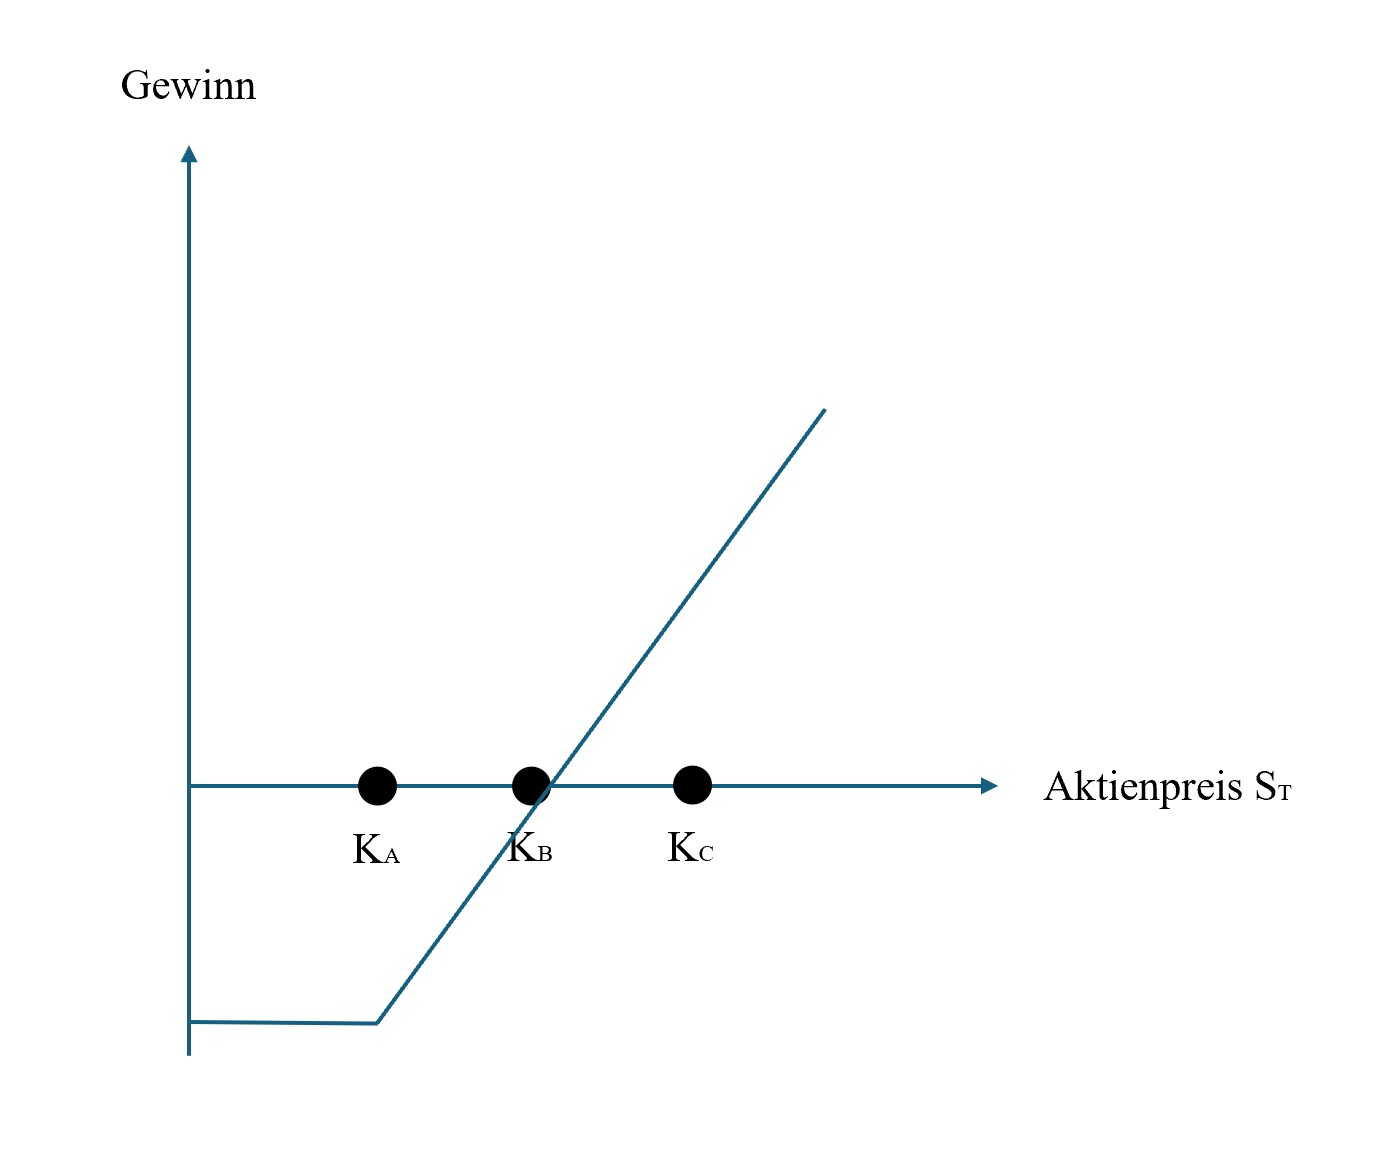
\includegraphics[width=7cm]{images/K_A.jpg}
    \caption{Gewinndiagramm der Call-Option mit $K=K_A$}
    \label{fig:K_A-butterfly}
  \end{minipage}
  \hfill
  \begin{minipage}[b]{0.4\textwidth}
    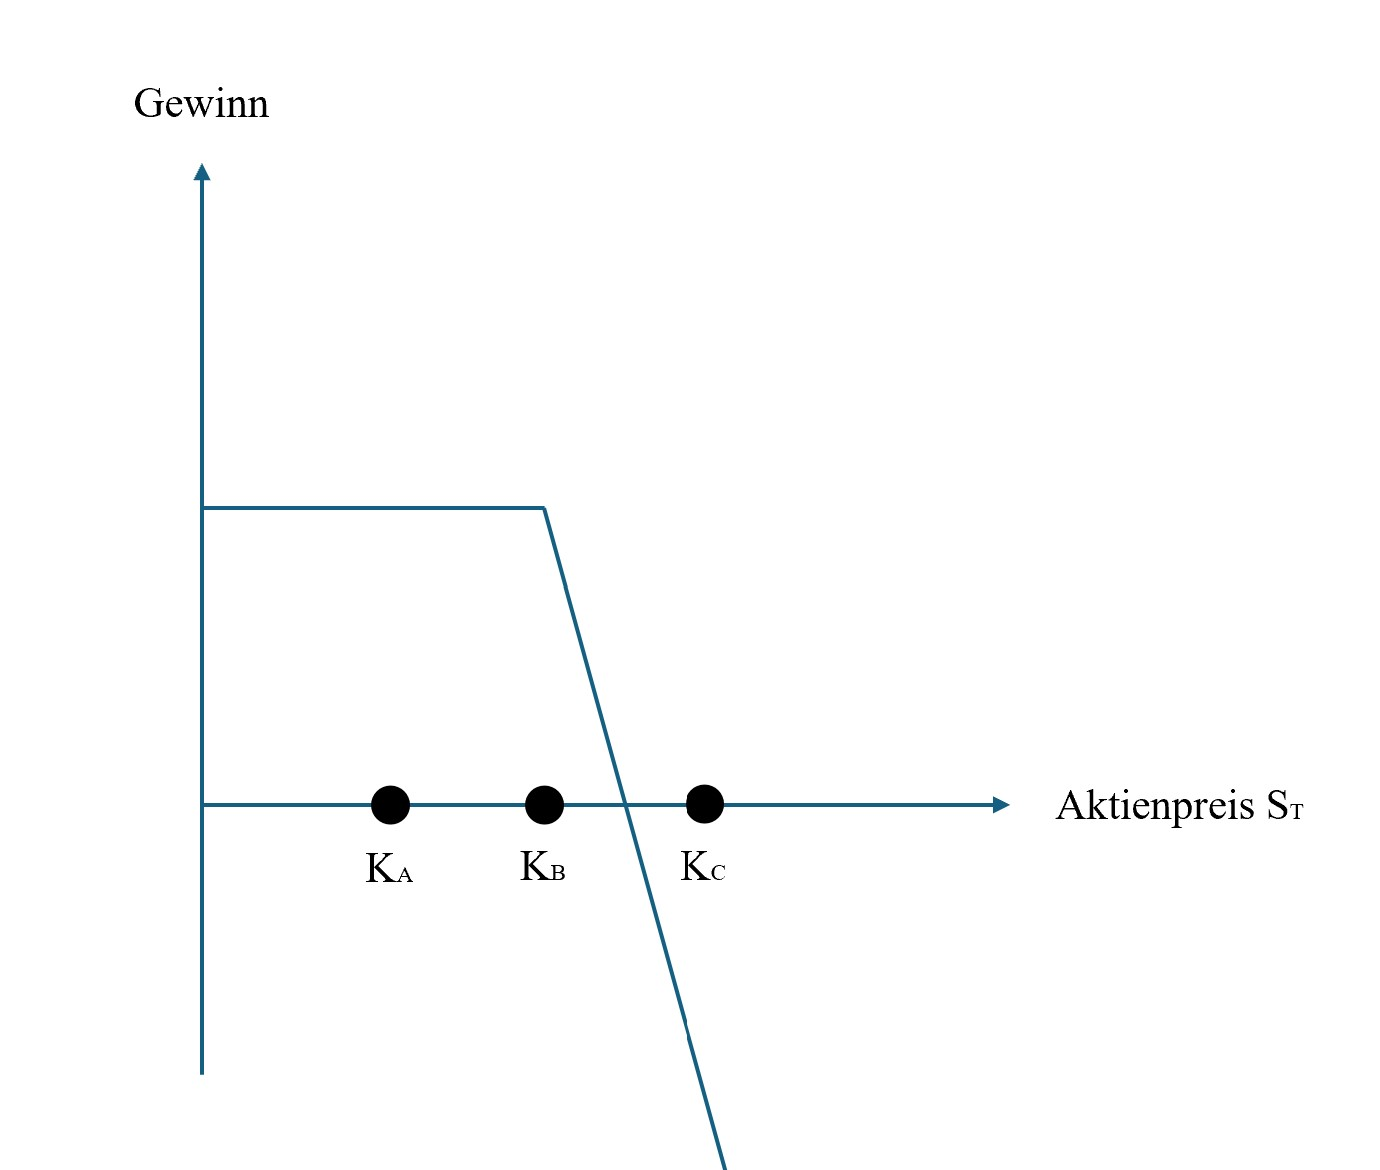
\includegraphics[width=7cm]{images/K_B.jpg}
    \caption{Gewinndiagramm der Call-Optionen mit $K=K_B$}
    \label{fig:K_B-butterfly}
  \end{minipage}
\end{figure}
\begin{figure}[H]
  \centering
  \begin{minipage}[b]{0.4\textwidth}
    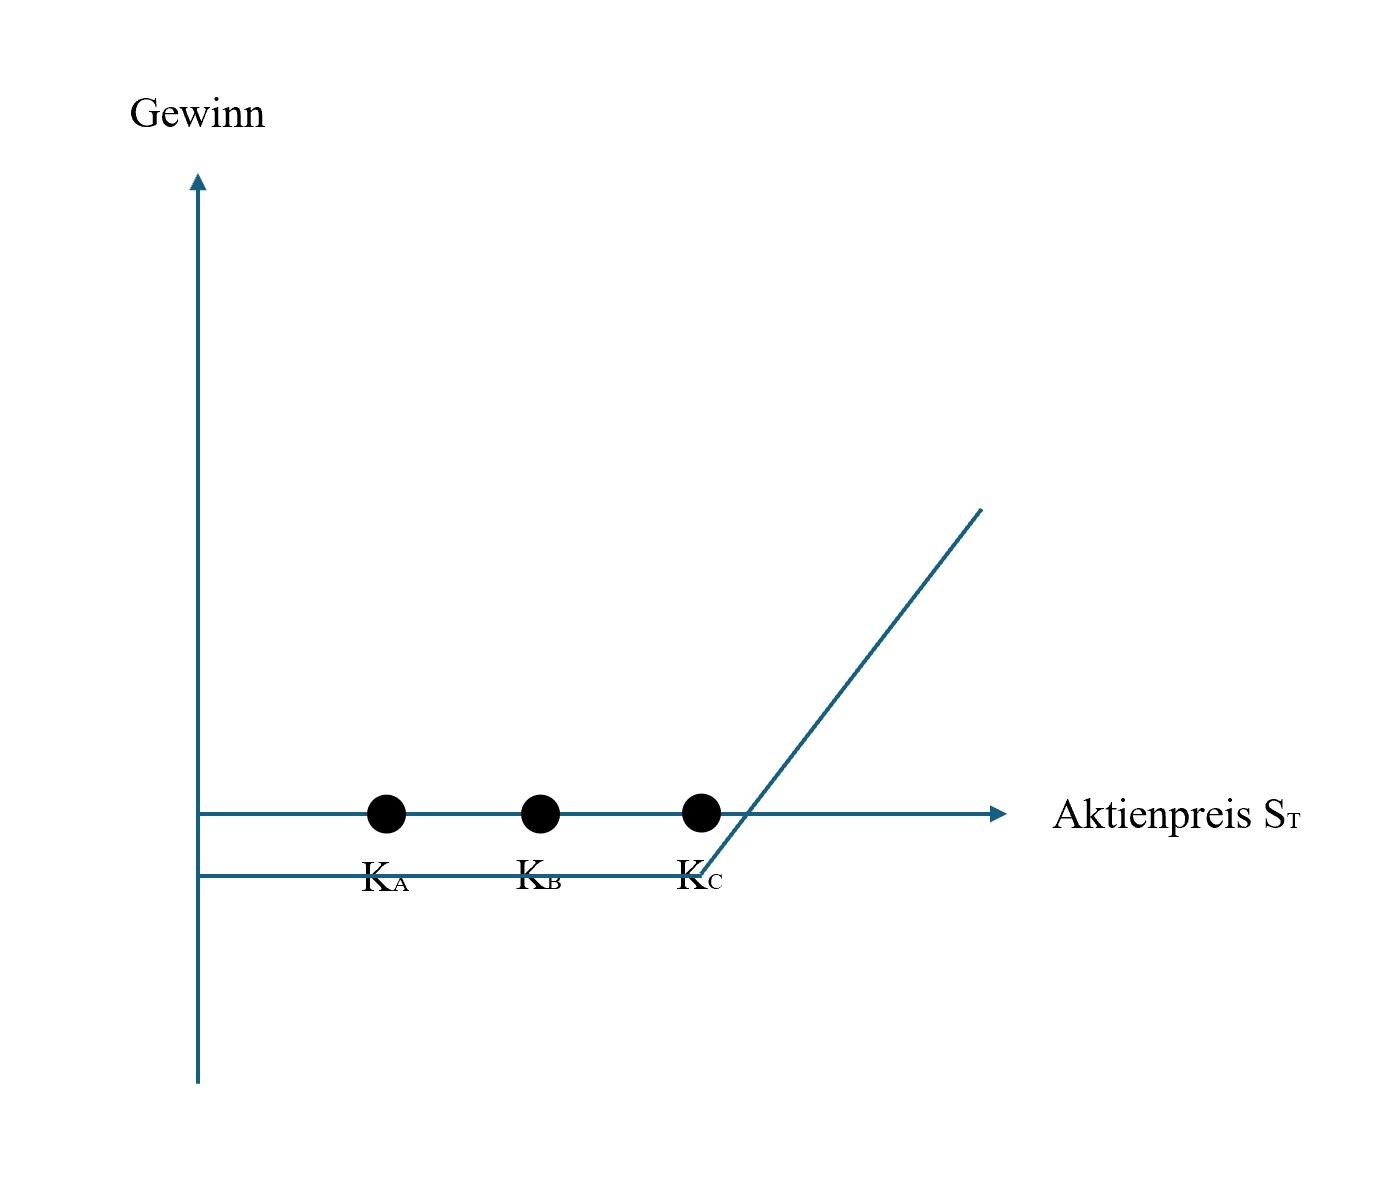
\includegraphics[width=7cm]{images/K_C.jpg}
    \caption{Gewinndiagramm der Call-Option mit $K=K_C$}
    \label{fig:K_C-butterfly}
  \end{minipage}
  \hfill
  \begin{minipage}[b]{0.4\textwidth}
    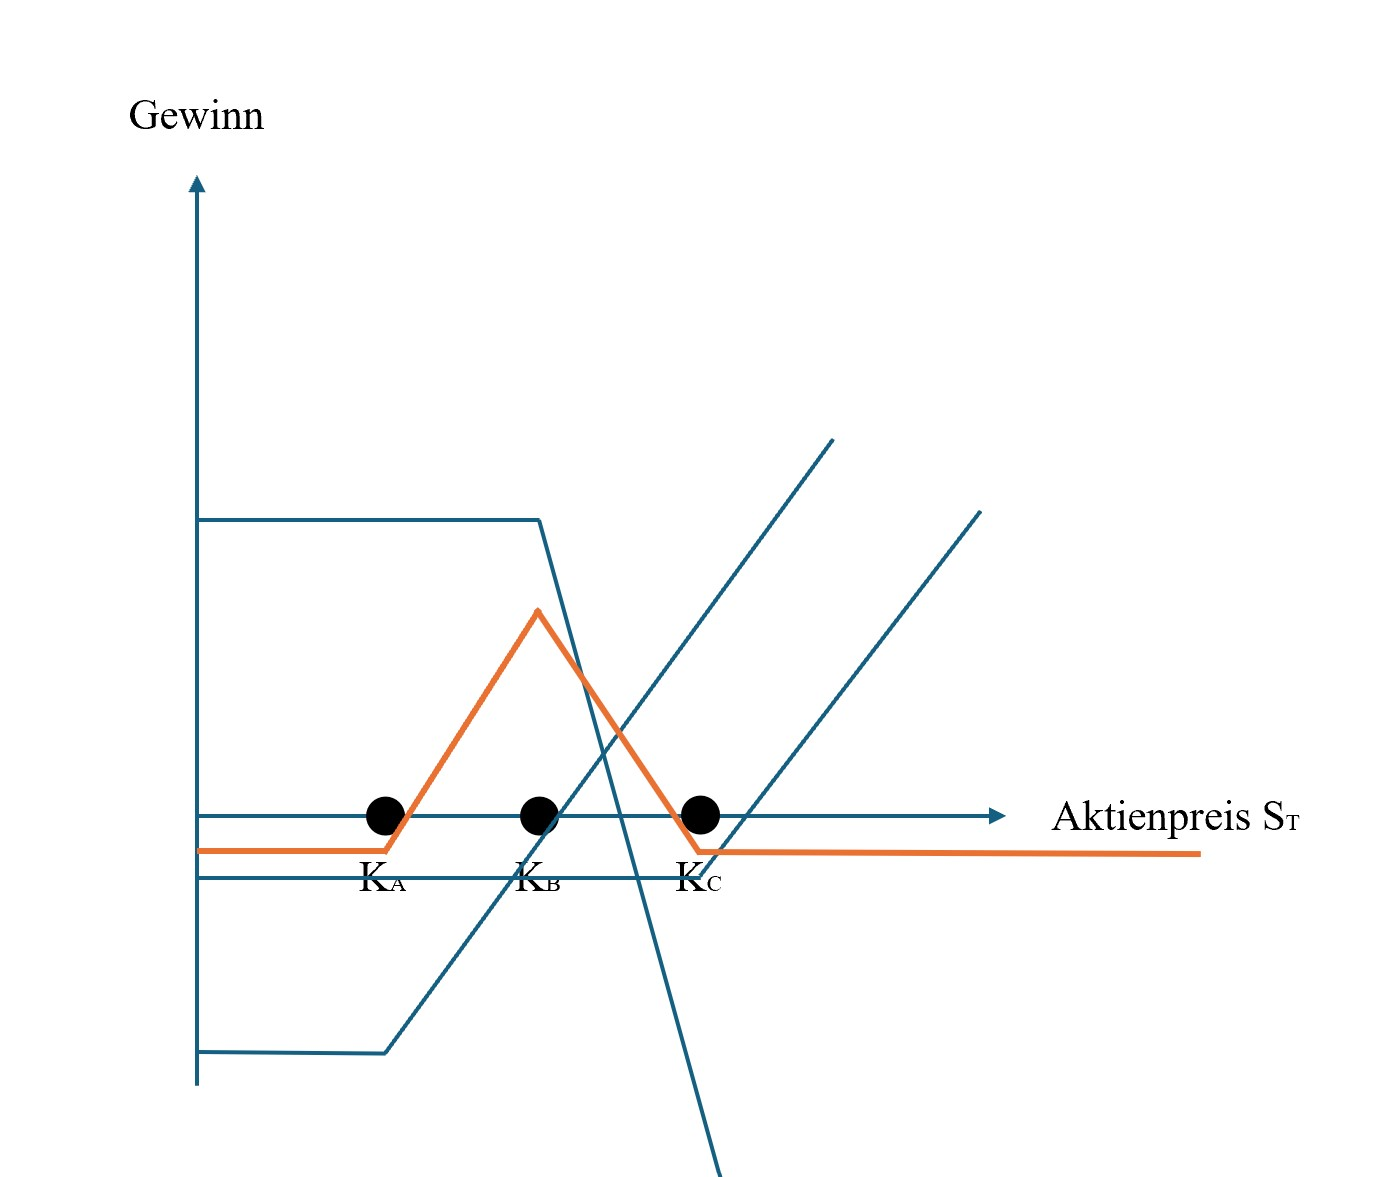
\includegraphics[width=7cm]{images/komplett-K_ABC.jpg}
    \caption{Gewinndiagramm des Long-Butterfly-Spreads}
    \label{fig:K_ABC-butterfly}
  \end{minipage}
\end{figure}
Abbildungen \ref{fig:K_A-butterfly}, \ref{fig:K_B-butterfly} und \ref{fig:K_C-butterfly} zeigen den Gewinn, der aus dem Kauf ($K=K_A$ und $K=K_C$) und Verkauf ($K=K_B$) der jeweiligen Optionen resultiert in Abhängigkeit des Aktienpreises. Abbildung \ref{fig:K_ABC-butterfly} zeigt das Gewinndiagramm, das entsteht, wenn man die Gewinne der einzelnen Optionen addiert und somit den Long-Butterfly-Spread erhält. Wie im Diagramm zu sehen, wettet man darauf, dass der Akienpreis zwischen $K_A$ und $K_C$ sein wird. \\\\Da Long-Butterfly-Spreads kein eigener Optionstyp sind und sich einfach aus mehreren Call- oder Put-Optionen zusammensetzen, braucht es für die Berechnung des Preises eines Long-Butterfly-Spreads keine neue Formeln.\\Kauft man für die Erzeugung eines Long-Butterfly-Spreads eine Call-Option mit Ausübungspreis $K_A$ für $C_A$, verkauft man zwei Calls mit $K=K_B$ für je $C_B$ und kauft man einen Call mit $K=K_C$ für $C_C$, so beträgt der Preis des Spreads $$\mathcal{B}_L=C_A-2C_B+C_C$$ Will man den Long-Butterfly-Spread aus Put-Optionen zusammenstellen, so kauft man eine Put-Option mit Ausübungspreis $K_A$ für $P_A$, verkauft zwei Puts mit $K=K_B$ für je $P_B$ und kauft einen Put mit $K=K_C$ für $P_C$. Somit beträgt der Preis des gesamten Long-Butterfly-Spreads $$\mathcal{B}_L=P_A-2P_B+P_A$$ (\cite{Kolb2009}).\\\\
Da man mit einem Long-Butterfly-Spread auf eine tiefe Volatilität wettet, sinkt sein Preis mit steigender Volatilität, was in Abbildung \ref{fig:sigma-B_L} erkennbar ist.
\begin{figure}[h]
    \centering
    \begin{tikzpicture}
        \begin{axis}[title=Long-Butterfly-Spread, xlabel=Volatilität $\sigma$ in \%, ylabel=$\mathcal{B}_L$ in \$, mark size = 0]
            \addplot+[
            scatter
            ]
            table[x index=0, y index=1]
            {B_L.dat};
        \end{axis}
    \end{tikzpicture}
    \caption{Einfluss der Volatilität auf den Preis eines Long-Butterfly-Spreads aus europäischen Call-Optionen mit Ausübungspreisen $K_A=80, K_B=100, K_C=120, t=1$ und $S_0=100, r=5.3\%$; berechnet mit den Black-Scholes-Formeln}
    \label{fig:sigma-B_L}
\end{figure} 

\subsection{Short-Butterfly-Spreads}
Neben Long-Butterfly-Spreads gibt es zudem Short-Butterfly-Spreads. Im Gegensatz zu Long-Butterfly-Spreads wettet man mit einem Short-Butterfly-Spread darauf, dass der Anlagekurs ausserhalb eines bestimmten Bereiches sein wird. Man wettet also auf eine hohe Volatilität des Anlagekurses. Man konstruiert den Spread so, indem man eine Option mit dem tiefen Ausübungspreis $K_A$ verkauft, zwei Optionen mit mittlerem Ausübungspreis $K_B$ kauft und eine Option mit hohem Ausübungspreis $K_C$ verkauft. Gleich wie Long-Butterfly-Spreads können Short-Butterfly-Spreads aus sowohl Call- als auch Put-Optionen bestehen (Butterfly (options), \cite{wikibutterfly2024}).
\begin{figure}[h]
    \centering
    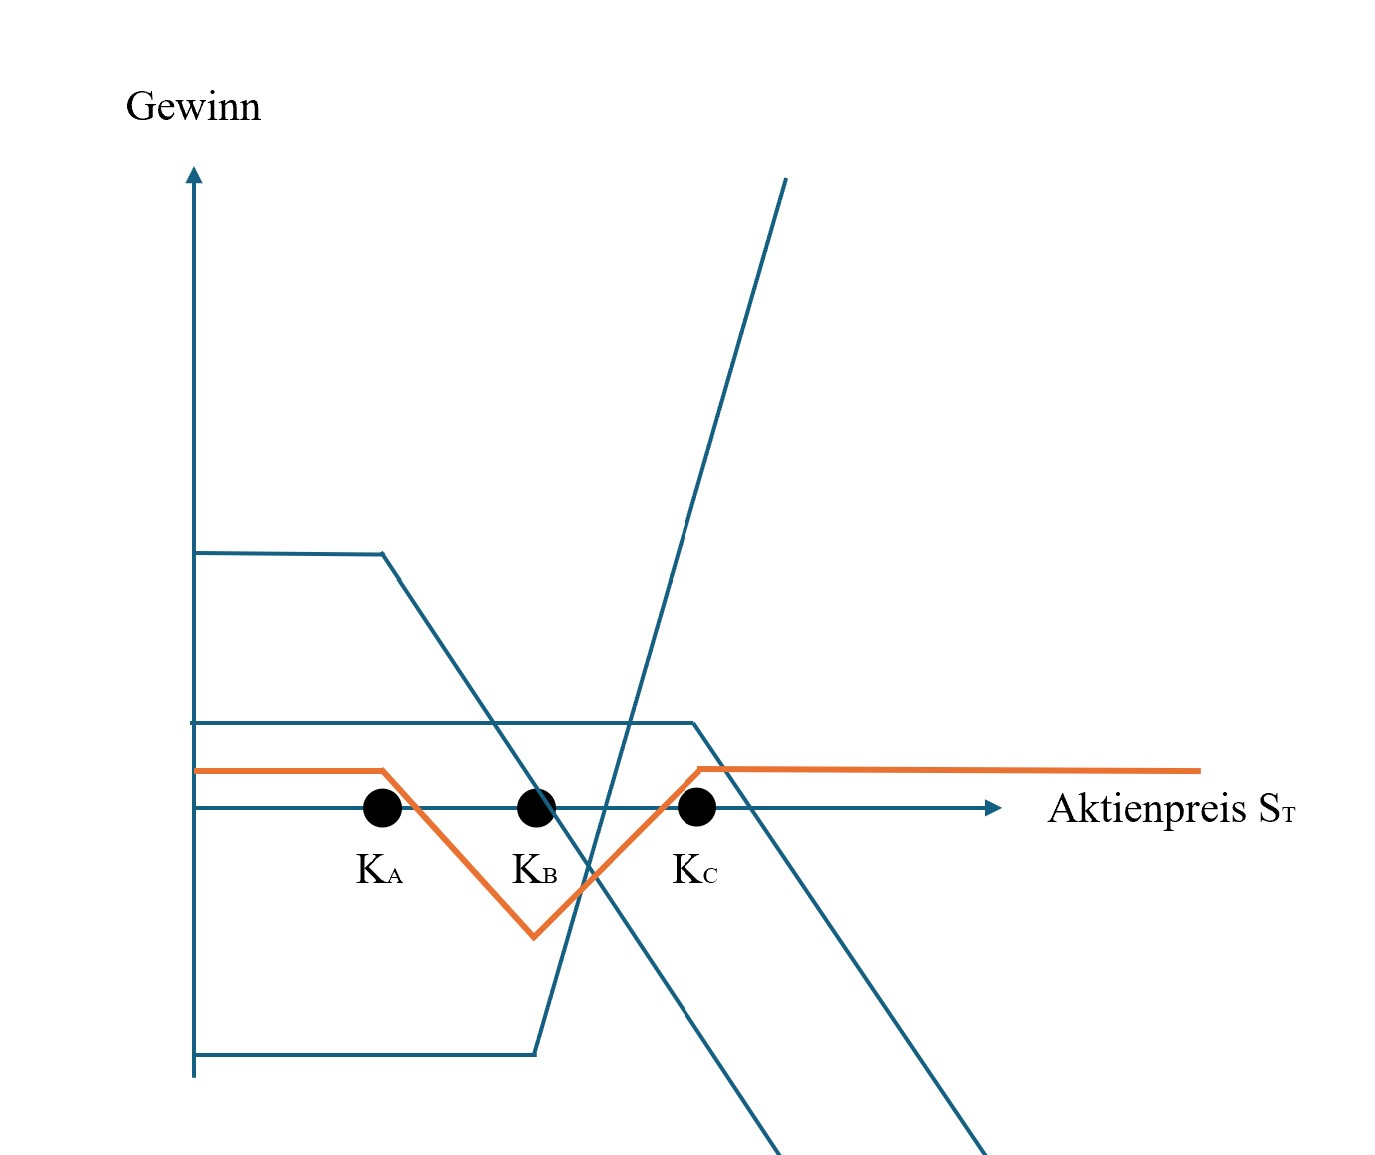
\includegraphics[width=0.5\linewidth]{images/short-butterfly-spread.jpg}
    \caption{Gewinndiagramm des Short-Butterfly-Spreads}
    \label{fig:short-butterfly}
\end{figure}
Abbildung \ref{fig:short-butterfly} zeigt den Gewinn des Short-Butterfly-Spreads in Abhängigkeit des Aktienpreises. Der Spread (orange eingezeichnet) wurde mithilfe der blau eingezeichneten Call-Optionen erzeugt. Man erkennt, dass mit dem Short-Butterfly-Spread darauf gehofft wird, dass der Anlagepreis tiefer als $K_A$ oder höher als $K_C$ sein wird, es wird somit auf eine hohe Volatilität gesetzt.\\\\Die Preise für Short-Butterfly-Spreads lassen sich wie bei Long-Butterfly-Spreads als Summe der Optionspreise, welche zur Erstellung des Spreads verwendet wurden, berechnen. Setzt sich der Spread aus Call-Optionen zusammen, so beträgt der Preis des Short-Butterfly-Spreads $$\mathcal{B}_S=-C_A+2C_B-C_C$$Besteht er aus Put-Optionen, beträgt der Preis $$\mathcal{B}_S=-P_A+2P_B-P_C$$ Man merkt, dass diese Preise stets negativ sind. Das rührt daher, dass Short-Positionen stets damit verbunden sind, Schulden zu machen. Diese Schulden muss man machen, um den Spread zu finanzieren. Dass der Preis des Short-Butterfly-Spreads negativ ist, heisst also, dass ich als Besitzer jemandem Geld \textit{bezahlen} müsste, dass dieser den Spread übernimmt. Ich muss dem neuen Besitzer Geld bezahlen, da dieser mit dem Spread automatisch auch die Schulden übernimmt, welche ich gemacht habe, um den Spread zu erstellen.

\section{Fantasieoptionen}
Bisher wurden in dieser Arbeit zwei Optionstypen besprochen: Call-Optionen und Put-Optionen. Call-Optionen haben einen Payoff von $$X=(S-K)^+$$und Put-Optionen haben einen Payoff von $$X=(K-S)^+$$ Die Theorie, die zur Herleitung der Pricing-Formeln geführt hat, funktioniert aber nicht nur für die beiden Payoff-Funktionen von Calls und Puts. Man kann auch Formeln für hypothetische Optionen herleiten, welche komplett andere Payoff-Funktionen haben.\\\\
Man stelle sich beispielsweise eine Option vor, die bei der Ausübung den Payoff $$X=\frac{(S-K)^2}{S+K}$$ erbringt.
\begin{figure}[H]
    \centering
    \begin{tikzpicture}
        \begin{axis}[title=Fantasieoption, xlabel=Aktienpreis $S_T$ in \$, ylabel=Payoff in \$, mark size = 0]
            \addplot+[
            scatter
            ]
            table[x index=0, y index=1]
            {fant.dat};
        \end{axis}
    \end{tikzpicture}
    \caption{Payoff-Diagramm der Fantasieoption mit $K=100$}
    \label{fig:payoff-fant}
\end{figure}
Abbildung \ref{fig:payoff-fant} zeigt den Payoff der Fantasieoption in Abhängigkeit des finalen Aktienpreises $S_T$. Der Graph besitzt ein Minimum bei $S_T=100$. Für kleiner bzw. grösser werdende $S_T$ 
 steigt der resultierende Payoff. Somit ist der Payoff der Fantasieoption jenem des Long-Butterfly-Spreads (siehe vorheriger Abschnitt) ähnlich, womit die Fantasieoption für steigende Volatiliät teurer werden müsste.\\\\Wenn die Fantasieoption im europäischen Stil erst am Ende der Ausübungsfrist ausgeübt werden kann, kann man für die Herleitung einer Pricing-Formel die Formel aus Abschnitt \ref{binom-modell-allg-form} verwenden:
\begin{align*}
    \mathcal{I}_0(X)&=e^{-rL}\sum_{\omega \in \Omega}X(\omega)\pi^{N_U(\omega)}(1-\pi)^{N_D(\omega)}
\end{align*}
Setzt man den oben definierten Payoff ein, erhält man
\begin{align*}
    \mathcal{I}_0(X)&=e^{-rL}\sum_{\omega \in \Omega}\frac{(S_T(\omega)-K)^2}{S_T(\omega)+K}\pi^{N_U(\omega)}(1-\pi)^{N_D(\omega)}\\
    &=e^{-rL}\sum_{\omega \in \Omega}\frac{(S_0u^{N_U(\omega)}d^{N_D(\omega)}-K)^2}{S_0u^{N_U(\omega)}d^{N_D(\omega)}+K}\pi^{N_U(\omega)}(1-\pi)^{N_D(\omega)}
\end{align*}
Auch hier gilt wieder die Binomialverteilung, womit die oben beschriebene Option als europäische Option folgenden Preis hätte:
$$\mathcal{I}_0(\text{Option})=e^{-rL}\sum_{k=0}^{T}\binom{T}{k}\frac{(S_0u^kd^{T-k}-K)^2}{S_0u^kd^{T-k}+K}\pi^k(1-\pi)^{T-k}$$
Um den Preis für dieselbe Option in amerikanischer Ausführung zu berechnen, muss man bei der allgemeinen rekursiven Vorgehensweise für die amerikanische Optionspreisberechnung einfach den Payoff ersetzen:
\begin{enumerate}
    \item $\mathcal{M}_T=\frac{(S_T-K)^2}{S_T+K}$
    \item $\mathcal{M}_k(\mathbb{X})=\max\left\{\frac{(S_k-K)^2}{S_k+K}, e^{-r\Delta t}\mathcal{E}_\Pi(\mathcal{M}_{k+1}(\mathbb{X})|\mathcal{P}_k)\right\}$\ für $k<T$
\end{enumerate}
\begin{figure}[H]
    \centering
    \begin{tikzpicture}
        \begin{axis}[title=Fantasieoption, xlabel=Aktienpreis $S_0$ in \$, ylabel=Optionspreis in \$, mark size = 0]
            \addplot+[
            scatter
            ]
            table[x index=0, y index=1]
            {S_0_fant.dat};
            \addplot+[
            scatter
            ]
            table[x index=0, y index=2]
            {S_0_fant.dat};
        \legend{Europäisch (Binomialmodell), Amerikanisch}
        \end{axis}
    \end{tikzpicture}
    \caption{Einfluss des Aktienpreises auf den Optionspreis der Fantasieoption für eine Aktie mit $K=240$, $T=20$, $L=1$, $r=5.3\%$, $\mu=-5.52\%$, $\sigma=65.9\%$. Die Kurven \textit{Europäisch (Binomialmodell)} und \textit{Amerikanisch} sind deckungsgleich.}
    \label{fig:S_0-fant}
\end{figure}
\begin{figure}[H]
    \centering
    \begin{tikzpicture}
        \begin{axis}[title=Fantasieoption, xlabel=Ausübungspreis $K$ in \$, ylabel=Optionspreis in \$, mark size = 0]
            \addplot+[
            scatter
            ]
            table[x index=0, y index=1]
            {K_fant.dat};
            \addplot+[
            scatter
            ]
            table[x index=0, y index=2]
            {K_fant.dat};
        \legend{Europäisch (Binomialmodell), Amerikanisch}
        \end{axis}
    \end{tikzpicture}
    \caption{Einfluss des Ausübungspreises auf den Optionspreis der Fantasieoption für eine Aktie mit $S_0=250$, $T=20$, $L=1$, $r=5.3\%$, $\mu=-5.52\%$, $\sigma=65.9\%$. Die Kurven \textit{Europäisch (Binomialmodell)} und \textit{Amerikanisch} sind deckungsgleich.}
    \label{fig:K-fant}
\end{figure}
Abbildungen \ref{fig:S_0-fant} und \ref{fig:K-fant} zeigen die Entwicklung des Optionspreises der oben beschriebenen Fantasieoption in Abhängigkeit des initialen Aktienpreises bzw. Ausübungspreises. Beide Graphen besitzen ein Minimum. Dieses Minimum scheint für $S_0\approx202$ und $K\approx234$ erreicht zu sein. Die europäischen und amerikanischen Optionspreise sind identisch. Dies führt zur Vermutung, dass es sich nie lohnen wird, die amerikanische Fantasieoption frühzeitig auszuüben. In dieser Hinsicht ist die Fantasieoption vergleichbar mit amerikanischen Call-Optionen.
\chapter{Pricing-Tool}
Zum gesamten Programm gehören fünf einzelne Skripte, welche alle in der Sprache Python geschrieben sind. $\texttt{get\_mu\_sigma.py}$ erhebt historische Kursdaten für die gewünschte Aktie und berechnet daraus die Drift $\mu$ und die Volatilität $\sigma$. $\texttt{binomial\_pricing.py}$ berechnet den europäischen Optionspreis mithilfe der Binomialformeln, $\texttt{american\_options\_pricing.py}$ den amerikanischen Optionspreis und $\texttt{european\_BS\_pricing.py}$ den europäischen Optionspreis mithilfe der Black-Scholes-Formeln. $\texttt{tool.py}$ generiert eine simple visuelle Benutzeroberfläche, wo man die gewünschte Art von Option und die nötigen Parameter eingibt. Anschliessend wird in einem Pop-up-Fenster das berechnete Resultat angezeigt.
\section{Berechnung von Drift und Volatilität}
Das Skript $\texttt{get\_mu\_sigma.py}$, welches sich im Anhang \ref{code:get_mu_sigma.py} befindet, beinhaltet die Methode $\texttt{yearly\_mu\_sigma(ticker)}$, welche als Argument den Kürzel der gewünschten Aktie nimmt und die jährliche Drift und die jährliche Volatilität ausgibt. Das Skript benutzt das Modul $\texttt{yfinance}$, um die Aktienkurse am Ende des Handelstags während des letzten Jahres herunterzuladen. Dafür ist die Zeile \begin{lstlisting}
stock_data = yf.download(ticker, start=start_date, end=end_date)
\end{lstlisting} verantwortlich, welche für die gewünschte Aktie alle Schlusskurse vom Datum vor einem Jahr bis heute herunterlädt. Die Zeilen \begin{lstlisting}
stock_data['Returns'] = stock_data['Adj Close'].pct_change()
pct_returns = stock_data['Returns'].dropna()
\end{lstlisting}
berechnen jeweils die prozentuale tägliche Rendite und löschen alle Einträge, welche keine Zahlen sind. \begin{lstlisting}
log_returns = []
for pct_return in pct_returns:
    log_returns.append(np.log(pct_return+1))
\end{lstlisting} rechnet die prozentualen täglichen Renditen in logarithmische tägliche Renditen um. Die Zeilen \begin{lstlisting}
mean_return_day = np.mean(log_returns)
std_dev_return_day = np.std(log_returns)

mu = (T_1/T_0)*mean_return_day
sigma = std_dev_return_day*np.sqrt(T_1/T_0)
\end{lstlisting} berechnen dann den Mittelwert und die Standardabweichung aller täglichen logarithmischen Renditen und rechnen sie nach den Formeln $$\mu_{T_1}=\frac{T_1}{T_0}\mu_{T_0}$$ und $$\sigma_{T_1}=\sqrt{\frac{T_1}{T_0}}\sigma_{T_0}$$ um, sodass man die jährliche Drift und die jährliche Volatilität der Aktie erhält.\\\\Der Programmcode von diesem Skript wurde teilweise von ChatGPT (persönliche Kommunikation, 5. April 2024) generiert. Der verwendete Prompt und die generierte Antwort findet sich im Anhang \ref{ai-tools}.
\section{Binomialformeln}
Das Skript $\texttt{binomial\_pricing.py}$, welches sich im Anhang \ref{code:binomial_pricing.py} befindet, beinhaltet die Methode $\texttt{euro\_bin\_price(ticker, time\_to\_maturity\_days, exercise\_price, step\_amount)}$, welche für den gegebenen Aktienkürzel, die Laufzeit in Tagen, den Ausübungspreis und die Anzahl Schritte im Modell den europäischen Call- und Put-Optionspreis mithilfe der Binomialformeln berechnet und ausgibt. Die Zeilen \begin{lstlisting}
stock = yf.Ticker(ticker)
S_0 = stock.info["currentPrice"]
(mu, sigma) = yearly_mu_sigma(ticker)
\end{lstlisting} laden den aktuellen Preis der gewünschten Aktie herunter und lassen mithilfe des Skripts $\texttt{get\_mu\_sigma.py}$ die Drift und die Volatilität berechnen. Der Code\begin{lstlisting}
u = np.exp(mu*(time_to_maturity_years/step_amount) + sigma*np.sqrt(time_to_maturity_years/step_amount))
d = np.exp(mu*(time_to_maturity_years/step_amount) - sigma*np.sqrt(time_to_maturity_years/step_amount))
pi = (np.exp(r*time_to_maturity_years/step_amount) - d)/(u - d)
\end{lstlisting} berechnet nach demselben Verfahren, das in Beispiel \ref{ex:u-d-derivation} verwendet wurde, die Faktoren $u$ und $d$.\footnote{Die Laufzeit wird von dem Benutzer in Tagen eingegeben und früher im Code in Jahre umgerechnet, sodass die Einheit der dabei verwendeten Variablen $\texttt{time\_to\_maturity\_years}$ stimmt.} Zudem wird die Martingalwahrscheinlichkeit $\pi$ berechnet, wie sie in Theorem \ref{th:binom-formulae} formuliert ist. In \begin{lstlisting}
sum1 = 0
for k in range(0, step_amount+1):
    sum1 += comb(step_amount, k)*max((S_0*u**k*d**(step_amount - k) - exercise_price), 0)*pi**k*(1 - pi)**(step_amount - k)
C_0 = np.exp(-r*time_to_maturity_years)*sum1
P_0 = C_0 + exercise_price*np.exp(-r*time_to_maturity_years) - S_0
\end{lstlisting}
wird mit der Formel in Theorem \ref{th:binom-formulae} der Call-Optionspreis $C_0$ und anschliessend mit der Put-Call-Parität (Theorem \ref{th:put-call-parity}) der Put-Optionspreis $P_0$ berechnet.

\section{Amerikanische Optionen}
Das Skript $\texttt{american\_options\_pricing.py}$, welches sich im Anhang \ref{code:american_options_pricing.py} befindet, beinhaltet drei Methoden: $\texttt{payoff(S, K)}$, welche in Abhängigkeit des Aktienpreises und des Ausübungspreises den Payoff liefert, $\texttt{snell(ups, downs, K, delta\_t)}$, welche für einen bestimmten Block im Zustandsbaum, den Ausübungspreis und die Länge eines Zeitintervalls $\Delta t$ den optimalen Wert ausgibt, und $\texttt{american\_option\_price(ticker, t\_days, K, T)}$, welche für den Aktienkürzel, die Laufzeit in Tagen, den Ausübungspreis und die Anzahl Schritte im Modell den amerikanischen Optionspreis berechnet.\\
Die Definition der Methode $\texttt{payoff(S, K)}$ spielt keine Rolle, da sie, je nachdem, ob der Preis einer Call- oder Put-Option gefordert wird, vom Skript $\texttt{tool.py}$ neu definiert wird.\\
Die Methode $\texttt{american\_option\_price(ticker, t\_days, K, T)}$ ist folgendermassen aufgebaut: Der Code\begin{lstlisting}
stock = yf.Ticker(ticker)
S_0 = stock.info["currentPrice"]
(mu, sigma) = get_mu_sigma.yearly_mu_sigma(ticker)
u = np.exp(mu*time_to_maturity/step_amount + sigma*np.sqrt(time_to_maturity/step_amount))
d = np.exp(mu*time_to_maturity/step_amount - sigma*np.sqrt(time_to_maturity/step_amount))
pi = (np.exp(r*time_to_maturity/step_amount) - d)/(u - d)
\end{lstlisting}
berechnet -- wie bei den Binomialformeln -- aus dem heruntergeladenen Aktienpreis und der generierten Drift und Volatilität sowohl die Faktoren $u$ und $d$ als auch die Martingalwahrscheinlichkeit $\pi$. Anschliessend gibt $\texttt{return snell(0, 0, K, time\_to\_maturity/step\_amount)}$ den optimalen Wert $\mathcal{M}_0$ zurück. Dieser wird mithilfe der Methode $\texttt{snell(ups, downs, K, delta\_t)}$ berechnet. Sie funktioniert folgendermassen: Sie nimmt als Argumente die Anzahl Auf- und Abbewegungen, die der Aktienkurs gemacht hat, den Ausübunspreis und die Länge eines Zeitintervalls. Für eine gegebene Anzahl Auf- und Abbewegungen wird der Aktienpreis mit \begin{lstlisting}
S = S_0*u**ups*d**downs
\end{lstlisting} berechnet. Anschliessend wird nach dem rekursiven Muster, welches in Theorem \ref{th:calc-snell-envelope} beschrieben wird, die Snell-Umhüllende berechnet: \begin{lstlisting}
if (ups + downs) == step_amount:
    return payoff(S, K)
elif (ups + downs) < step_amount:
    expected_snell = pi*snell(ups + 1, downs, K, delta_t) + (1 - pi)*snell(ups, downs + 1, K, delta_t)
    return max(payoff(S, K), np.exp(-r*delta_t)*expected_snell)
\end{lstlisting}Dabei wird für jede gegebene Anzahl Auf- und Abbwegegungen kontrolliert, ob man sich bereits in der letzten Schicht des Zustandbaumes befindet. Wenn ja, dann wird einfach der Payoff ausgegeben. Wenn nicht, dann wird der erwartete optimale Wert der nächsthöheren Schicht abgezinst und ausgegeben, wofür wiederum die Methode $\texttt{snell}$ angewendet wird. 

\section{Black-Scholes-Formeln}
Das Skript $\texttt{european\_BS\_pricing.py}$, welches sich im Anhang \ref{code:european_BS_pricing.py} befindet, beinhaltet die Methode $\texttt{european\_BS\_price(ticker, time\_to\_maturity\_days, exercise\_price)}$, die für den Aktienkürzel, Laufzeit in Tagen und den Ausübungspreis den Preis einer europäischen Call- und Put-Option berechnet und ausgibt. Mit \begin{lstlisting}
stock = yf.Ticker(ticker)
S_0 = stock.info["currentPrice"]
(mu, sigma) = yearly_mu_sigma(ticker)
\end{lstlisting} wird der aktuelle Aktienpreis heruntergeladen und die Drift und Volatilität berechnet. Gemäss Theorem \ref{th:black-scholes-formulae} werden mit \begin{lstlisting}
d_1 = 1/(sigma*np.sqrt(time_to_maturity_years))*(np.log(S_0/exercise_price) + time_to_maturity_years*(r + sigma**2/2))
d_2 = d_1 - sigma*np.sqrt(time_to_maturity_years)
\end{lstlisting} die beiden Parameter $d_1$ und $d_2$ berechnet. Mithilfe der Black-Scholes-Formeln in Theorem \ref{th:black-scholes-formulae} werden schliesslich durch den Code\begin{lstlisting}
C_0 = float(S_0*stats.norm.cdf(d_1) - np.exp(-r*time_to_maturity_years)*exercise_price*stats.norm.cdf(d_2))
P_0 = float(-S_0*stats.norm.cdf(-d_1) + np.exp(-r*time_to_maturity_years)*exercise_price*stats.norm.cdf(-d_2))
\end{lstlisting}Call- und Put-Optionspreis berechnet. Hierbei wird das Modul $\texttt{scipy}$ benutzt, um die Werte der Verteilungsfunktion $\texttt{stats.norm.cdf}$ zu erhalten.

\section{Pricing-Tool}
Das Skript \texttt{tool.py}, welches sich in voller Länge im Anhang \ref{code:tool.py} befindet, ist für die graphische Benutzeroberfläche verantwortlich. Die Benutzeroberfläche wird hierbei mithilfe des Moduls \texttt{tkinter} generiert. Mithilfe des Codes \begin{lstlisting}
wn = Tk()
wn.title("Optionspreisrechner")
wn.geometry("300x450")
...
wn.mainloop()
\end{lstlisting} wird das Fenster generiert. Der Ausdruck $\texttt{wn.mainloop()}$ befindet sich ganz am Ende des Skripts und sorgt dafür, dass das Fenster so lange existiert, bis das Programm von dem Benutzer beendet wird oder er das Fenster manuell schliesst. Der Code \begin{lstlisting}
option_method_var = tk.StringVar(value="")
option_method_lbl = Label(wn, text="Berechnungsmethode:").pack()
ttk.Radiobutton(wn, text="Europaeisch (Black-Scholes)", variable=option_method_var, value="BS").pack()
ttk.Radiobutton(wn, text="Europaeisch (Binomialmodell)", variable=option_method_var, value="Binomial").pack()
ttk.Radiobutton(wn, text="Amerikanisch", variable=option_method_var, value="American").pack()
\end{lstlisting} generiert sogenannte Radiobuttons, von denen der Nutzer einen auswählen kann, um sich zu entscheiden, ob der Optionspreis mit einer Black-Scholes-Formel, einer Binomialformel oder als amerikanischer Optionspreis berechnet wird. Zusätzlich werden zwei Radiobuttons generiert, um auszuwählen, ob der Call- oder der Put-Optionspreis berechnet werden soll. Mit \begin{lstlisting}
ticker_entry_lbl = Label(wn, text="Aktiensymbol:").pack()
ticker_entry = Entry(wn)
ticker_entry.pack()
\end{lstlisting} wird ein Eingabefeld generiert, wo der Benutzer den Aktienkürzel eingeben kann. Das Eingabefeld wird zudem beschriftet. Auf dieselbe Art werden Eingabefelder für Ausübungspreis, Laufzeit und Modellschrittanzahl generiert. Mit \begin{lstlisting}
submit_data_btn = Button(wn, text="BERECHNEN", command=submit_values)
submit_data_btn.pack()
\end{lstlisting} wird ein Knopf mit der Aufschrift \textit{BERECHNEN} generiert, der, wenn er gedrückt wird, die Methode \texttt{submit\_values} auslöst. Diese Methode funktioniert folgendermassen: Der Code in \begin{lstlisting}
try:
    selected_option_method = option_method_var.get()
    selected_option_type = option_type_var.get()
except:
    messagebox.showerror(title="Fehler", message="Es fehlen noetige Angaben.")
try:
    ticker = str(ticker_entry.get())
    exercise_price = float(exercise_price_entry.get())
    time_to_maturity_days = float(time_to_maturity_entry.get())
    if selected_option_method in ("Binomial", "American"):
        steps = int(steps_entry.get())
except:
    messagebox.showerror(title="Fehler", message="Ueberpruefe die Eingaben noch einmal!")
\end{lstlisting} speichert die eingegebenen Werte und öffnet gegebenenfalls ein Pop-up-Fenster, dass dem Benutzer mitteilt, dass er falsche oder ungenügende Werte eingegeben hat. Mit \begin{lstlisting}
if selected_option_method == "BS" and selected_option_type == "Call":
    show(european_BS_price(ticker, time_to_maturity_days, exercise_price)[0], "Europaeisch (Black-Scholes)", "Call")
elif selected_option_method == "Binomial" and selected_option_type == "Call":
    show(euro_bin_price(ticker, time_to_maturity_days, exercise_price, steps)[0], "Europaeisch (Binomialmodell)", "Call")
elif selected_option_method == "American" and selected_option_type == "Call":
    am.payoff = payoff_call
    show(am.american_option_price(ticker, time_to_maturity_days, exercise_price, steps), "Amerikanisch", "Call")
elif selected_option_method == "BS" and selected_option_type == "Put":
    show(european_BS_price(ticker, time_to_maturity_days, exercise_price)[1], "Europaeisch (Black-Scholes)", "Call")
elif selected_option_method == "Binomial" and selected_option_type == "Put":
    show(euro_bin_price(ticker, time_to_maturity_days, exercise_price, steps)[1], "Europaeisch (Binomialmodell)", "Put")
elif selected_option_method == "American" and selected_option_type == "Put":
    am.payoff = payoff_put
    show(am.american_option_price(ticker, time_to_maturity_days, exercise_price, steps), "Amerikanisch", "Put")
\end{lstlisting} wird für jede mögliche Kombination aus Optionstyp und gewünschter Berechnungsformel die Methode \texttt{show(calculated\_price, option\_method, option\_type)} aufgerufen. Wenn der amerikanische Optionspreis gewünscht wird, wird die Methode \texttt{payoff} im Skript $\texttt{american\_options\_pricing.py}$ überschrieben und so angepasst, dass entweder der Call- oder der Put-Preis berechnet wird -- je nachdem, was der Benutzer angewählt hat.\\Die Methode \texttt{show(calculated\_price, option\_method, option\_type)} generiert ein Pop-up-Fenster, das den berechneten Optionspreis anzeigt:\begin{lstlisting}
def show(calculated_price, option_method, option_type):
    messagebox.showinfo(title="Resultat", message=(option_type + "-Optionspreis " + option_method + ": $" + str(round(calculated_price, 2))))
\end{lstlisting}
Abbildungen \ref{fig:option-calc-tool}, \ref{fig:result-popup} und \ref{fig:tool-error} zeigen Screenshots der Benutzeroberfläche und der Pop-up-Fenster.
\begin{figure}
    \centering
    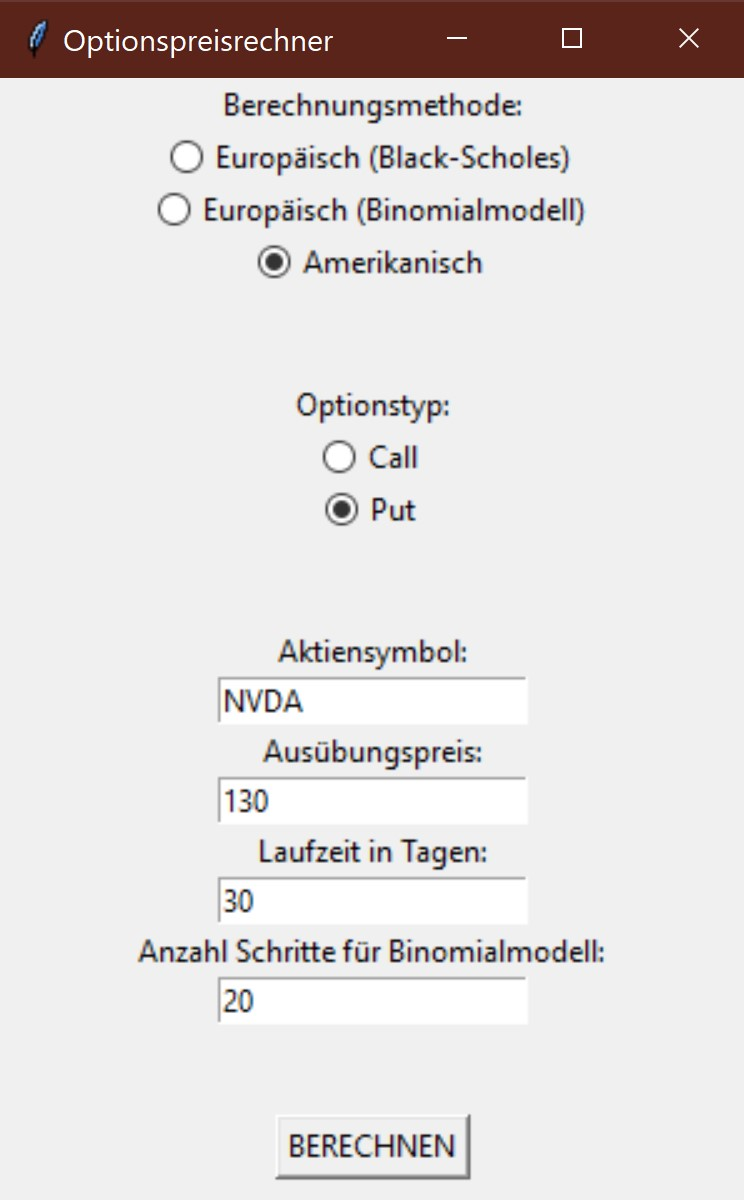
\includegraphics[width=0.4\linewidth]{images/option-calc-tool.jpg}
    \caption{Screenshot der Benutzerfläche des Pricing-Tools}
    \label{fig:option-calc-tool}
\end{figure}
\begin{figure}
    \centering
    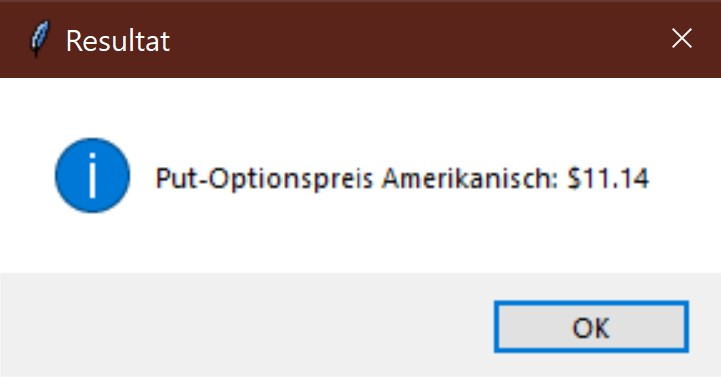
\includegraphics[width=0.4\linewidth]{images/result-popup.jpg}
    \caption{Screenshot des Pop-up-Fensters mit berechnetem Optionspreis}
    \label{fig:result-popup}
\end{figure}
\begin{figure}
    \centering
    
\includegraphics[width=0.4\linewidth]{images/ueberpruefe-eingaben-popup.jpg}
    \caption{Screenshot des Pop-up-Fensters mit Fehleranzeige}
    \label{fig:tool-error}
\end{figure}

\chapter{Diskussion}
\section{Modellkritik}
Bei der Herleitung der Pricing-Formeln wurden viele Annahmen gemacht, welche die Realität vereinfachen und somit erst ermöglichen, dass einfache Formeln hergeleitet werden können. Diese Annahmen sind jedoch oft unrealistisch. \textcite{Janková2018} nennt als Hauptkritikpunkt die als konstant angenommene Volatilität. So hange die Volatilität mit den Transaktionskosten\footnote{Kosten, die anfallen, wenn die Anlage verkauft oder gekauft wird. Die Transaktionskosten wurden in der in dieser Arbeit verwendeten Theorie als inexistent angenommen, was ebenfalls von \textcite{Janková2018} kritisiert wird.} und dem Handelsvolumen\footnote{Der Umsatz, der mit dem Handel der Anlage innerhalb eines Zeitraumes gemacht wird (Handelsvolumen (Börse), \cite{wikihandelsvolumen2023})} zusammen, was nicht in der Theorie berücksichtigt wird. Zusätzlich kann man an der Theorie, wie sie in dieser Arbeit besprochen wurde, kritisieren, dass man keinen allgemeingültigen Wert für den risikolosen Zinssatz hat. In dieser Arbeit wurde jeweils der Zinssatz der 3 Month Treasury Bill genommen, jedoch könnte man stattdessen auch beispielsweise britische oder Schweizer Staatsanleihen nehmen. Zudem wurde in der Theorie dieser Arbeit nicht berücksichtigt, dass viele Unternehmen regelmässig ihren Aktionären eine Dividende auszahlen. Diese Dividende hat einen Einfluss auf die Menge an Geld, die mit einer Aktie verdient werden kann, womit die Dividende auch den Optionspreis beinflusst. Es gibt Varianten der Black-Scholes-Formeln, welche Dividenden berücksichtigen, diese wurden aber nicht in dieser Arbeit behandelt. Ein weiterer Kritikpunkt wäre die Annahme, dass der Aktienkurs nur entweder steigen oder fallen kann. Im sogenannten \textit{Trinomialmodell} wird angenommen, dass der Kurs fallen, sinken und stagnieren kann. \textcite{Josheski2020} haben Binomial- und Trinomialmodell verglichen und sind zum Schluss gekommen, dass das sich die berechneten Optionspreise im Trinomialmodell schneller den Black-Scholes-Preisen annähern als Binomialmodellpreise. Das heisst, dass vor allem für kleine Modellschrittanzahlen das Trinomialmodell genauere Optionspreise liefert. Für grössere Modellschrittanzahlen verwendet man hingegen wieder vermehrt das Binomialmodell, da die benötigte Rechenzeit im Trinomialmodell sehr stark wächst im Vergleich zum Binomialmodell.
\\Jede weitere vereinfachende Annahme kann und soll man kritisch hinterfragen. Nichtsdestotrotz helfen sie, einfach und trotzdem genau Optionspreise zu berechnen. 

\section{Methodik und Arbeitsprozess}
\subsection{Arbeitsplanung}
Der Arbeitsprozess dieser Arbeit wurde zwar in der Projektvereinbarung grob skizziert, jedoch habe ich mich nicht exakt daran gehalten. In der Projektvereinbarung wurde festgelegt, dass bis Ende Sommerferien, dem 11. August 2024, alle Theorie erarbeitet und verschriftlicht sein soll. Dies wurde im Grossen und Ganzen auch erreicht, jedoch war laut Projektvereinbarung der Plan, die Theorie parallel zur Lektüre zu verschriftlichen. Dies wurde nicht so umgesetzt. Die Theorie von \textcite{Adelmeyer2003} und \textcite{Roman2012-sk} war bereits Anfang Mai gelesen, jedoch begann ich erst dann mit der Verschriftlichung der Theorie. Im Nachhinein stellte sich das als bessere Alternative heraus, da ich so gezwungen war, die Theorie ein zweites Mal vollständig durchzugehen, womit sich mein Verständnis nochmals merklich verbesserte. Ein Kritikpunkt meiner Arbeitsplanung hingegen ist die Programmierung des Pricing-Tools. Geplant war, die Programmierung erst nach den Sommerferien zu starten. Jedoch begann ich bereits im April damit, erste Fassungen des Pricing-Tools zu schreiben. Die ersten Versionen basierten auf der Theorie von \textcite{Adelmeyer2003}, welche leicht anders funktioniert als jene von \textcite{Roman2012-sk}, auf welcher ich schlussendlich diese Arbeit aufbaute. Somit entstanden mehrere Pricing-Tool-Versionen, welche unnötigerweise programmiert wurden und nicht ins Endprodukt einflossen. Hätte ich tatsächlich erst nach den Sommerferien mit der Pricing-Tool-Programmierung begonnen, hätte ich also Zeit sparen können, indem ich nur die Theorie von \textcite{Roman2012-sk} implementiert hätte.
\subsection{Autodidaktik}
Der Autodidaktikprozess funktionierte besser, als ich erwartet hätte. Es gab zwar während der Lektüre einige Fragen, diese konnten jedoch fast alle im Gespräch oder über eine Teams-Konversation mit Herrn Berchtold geklärt werden. Kritisieren muss ich am Autodidaktikprozess, dass ich die Theorie vor allem beim ersten Durchgang genauer hätte lesen sollen, sodass die Verschriftlichung anschliessend reibungsloser und schneller funktioniert hätte. Da das Buch von Roman (2012) grundsätzlich für Universitätsstudenten geschrieben ist, gab es hie und da Erklärungen, die schlichtweg zu kompliziert für meinen Wissensstand waren. Wie bereits erwähnt, besprach ich Schwierigkeiten grundsätzlich mit Herrn Berchtold. Jedoch gab es auch Stellen, die ich in die Arbeit übertragen musste, ohne sie zu 100\% verstanden zu haben. Dabei handelte es sich hauptsächlich um die Beweise \ref{proof:piecing-tg-stoptimes} und \ref{proof:fund-th-arb-theo}, die ich nicht gut genug verstanden habe, um sie völlig in eigene Worte umzuschreiben oder gar neu zu erfinden. Nach der Überarbeitung der Arbeit im Oktober hat sich jedoch mein Verständnis nochmals verbessert, sodass ich jede theoretische Überlegung im Hauptteil vollständig verstanden zu haben glaube. Im Anhang befinden sich einige Beweise, die ich sehr schwierig fand und einfach der Vollständigkeit wegen Teil der Arbeit sein mussten.
\subsection{Verschriftlichung der Theorie}
Die Verschriftlichung der Theorie war zu Beginn sehr schwierig für mich, da ich bis anhin noch die eine derartige Arbeit geschrieben hatte. Es war mir nicht klar, wie ich beginnen sollte, welche Mathematik- und Finanzkenntnisse ich bei den Lesern voraussetzen durfte und was in der Theorie relevant für meine Arbeit ist und was nicht. Ich probierte eine Woche lang, anzufangen, bis ich Herrn Berchtold nach einem Gespräch fragte, um nochmals über die Vorgehensweise zu sprechen. Nach der Besprechung konnte ich mir besser vorstellen, wie ich die Verschriftlichung der Theorie angehen sollte und konnte beginnen. Nachdem ich dann angefangen hatte, funktionierte es sehr gut. Jedoch war es teilweise schwierig, den passenden deutschen Begriff zu finden für Konzepte, die ich vor der Lektüre von \textcite{Roman2012-sk}, welche in englischer Sprache stattfand, noch nicht gekannt hatte (z. B. \textit{Snell-Umhüllende} oder \textit{Gesetz des Einheitspreises}). Eine Onlinesuche half jedoch in den allermeisten Fällen, die passende Übersetzung zu finden. Nachdem ich alles verschriftlicht hatte, ging ich die gesamte von mir geschriebene Theorie ein zweites Mal durch, um gewisse Ergänzungen zum besseren Verständnis des Lesers zu machen. Dies erwies sich im Nachhinein als förderlich, da ich die Arbeit so teilweise umstrukturieren und -- in meinen Augen -- verständlicher machen konnte. 
\subsection{Programmierung des Pricing-Tools}
Wie bereits erwähnt, ist wohl der grösste Kritikpunkt bei der Programmierung des Pricing-Tools, dass ich mehrere Versionen des Pricing-Tools geschrieben habe, welche auf der Theorie von Adelmeyer und Warmuth (2003) basierten. Da ich mich schlussendlich dazu entschieden habe, die Theorie von Roman (2012) in der Arbeit zu behandeln, musste ich eine neue Version des Pricing-Tools programmieren, welche die Pricing-Formeln von Roman (2012) benutzt. Ein weiterer Kritikpunkt beim Pricing-Tool ist, dass der berechnete Optionspreis in einem separaten Pop-up-Fenster angezeigt wird. Es wäre nutzerfreundlicher gewesen, eine Möglichkeit zu finden, dass der berechnete Optionspreis ebenfalls im Pricing-Tool-Fenster angezeigt wird. Zudem sind die Standardbenutzeroberflächen, die vom Modul \texttt{tkinter} generiert werden, im Design veraltet. So wäre es möglicherweise optisch ansprechender gewesen, ein anderes Modul zu verwenden (z. B. \texttt{kivy} oder \texttt{PyQt}). Mit anderen, zusätzlichen Modulen (und deutlich mehr Zeit) hätte ich unter Umständen mehr Freiheiten bezüglich der Gestaltung der Benutzeroberfläche gehabt und je nachdem sogar die Möglichkeit, das Pricing-Tool als App für das Smartphone oder als Web-App der Allgemeinheit zur Verfügung zu stellen. Ich bin jedoch bisher nur mit \texttt{tkinter} vertraut und hätte mir das Umgehen mit anderen Modulen zuerst aneignen müssen. Was man sonst noch kritisieren könnte am Pricing-Tool, ist die programmiertechnische Umsetzung der Berechnung von amerikanischen Optionspreisen. Die Rechenzeit für grössere Schrittanzahlen $T$ wächst sehr stark im Vergleich zu europäischen Optionen (siehe Abbildung \ref{fig:runtime}), was möglicherweise mit besseren Informatikkenntnissen verbessert werden könnte.
\begin{figure}[h]
    \centering
    \begin{tikzpicture}
        \begin{axis}[title=Rechenzeit, xlabel=Schrittanzahl $T$, ylabel=Rechenzeit in Sekunden, mark size = 0]
            \addplot+[
            scatter
            ]
            table[x index=0, y index=1]
            {runtime.dat};
            \addplot+[
            scatter
            ]
            table[x index=0, y index=2]
            {runtime.dat};
        \legend{Europäisch (Binomialmodell), Amerikanisch}
        \end{axis}
    \end{tikzpicture}
    \caption{Benötigte Rechenzeit für die Berechnung von europäischen und amerikanischen Optionspreisen in Abhängigkeit der Schrittanzahl $T$}
    \label{fig:runtime}
\end{figure}

\chapter{Zusammenfassung}
\section{Thematik}
Das Ziel dieser Arbeit war, Methoden zur Optionspreisberechnung mathematisch zu behandeln und deren Herleitung so verständlich zu formulieren, dass ein Mitschüler an der Kantonsschule sie verstehen könnte. Namentlich wurde die Berechnung von europäischen Put- und Call-Optionspreisen mithilfe des Binomialmodells und mithilfe der Black-Scholes-Formeln, die rekursive Berechnung von amerikanischen Put- und Call-Optionspreisen als auch die Berechnung von europäischen und amerikanischen Optionspreisen mit beliebig gewählten Payoff-Funktionen mithilfe des Binomialmodells behandelt. Zudem wurden Long- und Short-Butterfly-Spreads und deren Verwendung und Preisberechnung besprochen. Es wurde der Einfluss von verschiedenen Parametern, wie beispielsweise der Volatilität, des Ausübungspreises oder der Laufzeit, auf den Optionspreis untersucht, graphisch dargestellt und auch mathematisch hergeleitet. In diesem Zusammenhang wurden auch die sogenannten \textit{Griechen} -- wichtige Kennzahlen in der Finanzanalyse -- hergeleitet. Es wurde mithilfe von Python ein Programm geschrieben, das für eingegebene Parameter den gewünschten Optionspreis berechnet. Es wurde ebenfalls eine graphische Benutzeroberfläche programmiert, die dem Benutzer des Programms die Verwendung erleichtert und anschaulicher macht.

\section{Vorgehensweise und Ergebnisse}
Die Herleitung der Theorie folgt dem Buch von \textcite{Roman2012-sk}. Nachdem ich zuerst die Theorie von \textcite{Adelmeyer2003} und anschliessend \textcite{Roman2012-sk} durchgelesen habe, begann das Aufschreiben der Theorie in möglichst eigenen Worten. Parallel entstanden die ersten Versionen des Pricing-Tools, die letztlich aber nicht ins Endresultat einflossen. Nach dem Verfassen der Herleitung der Pricing-Formeln begann das Verfassen der Kapitel zum Einfluss der Parameter auf den Optionspreis und der Preisberechnung von Optionen mit anderen Payoff-Strukturen. Schliesslich wurde die mittlerweile fertiggestellte Programmierung des Pricing-Tools dokumentiert. Die hergeleiteten Pricing-Formeln finden sich in Theorem \ref{th:binom-formulae} (Binomialmodellformeln), Theorem \ref{th:black-scholes-formulae} (Black-Scholes-Formeln) und Theorem \ref{th:calc-snell-envelope} (amerikanische Optionspreise). Für den Einfluss der Parameter auf die Optionspreise gilt: Für eine steigende Modellschrittanzahl nähert sich der Binomialpreis dem Black-Scholes-Preis und der amerikanische Put-Preis einem anderen, leicht höheren Preis. Für steigende Aktienpreise steigt der Call-Preis und sinkt der Put-Preis. Für steigende risikolose Zinssätze steigt der Call-Preis und sinkt der Put-Preis. Für steigende Ausübungspreise hingegen sinkt der Call-Preis und steigt der Put-Preis. Für eine steigende Volatilität wächst sowohl der Call- als auch der Put-Preis. Für eine steigende Laufzeit steigt der Call-Preis, wobei über den Put-Preis keine allgemeine Aussage gemacht werden kann. Der amerikanische Optionspreis ist stets mindestens so gross wie der europäische, da eine amerikanische Option ihrem Inhaber mindestens genauso viele Rechte bringt wie eine entsprechende europäische. Amerikanische Call-Preise sind stets gleich hoch wie europäische Call-Preise für dieselbe Option. Es wurde zudem herausgefunden, dass, der Erwartung entsprechend, der Preis eines Long-Butterfly-Spreads für eine steigende Volatilität sinkt. 

\section{Diskussion}
Es wurde besprochen, dass die vielen vereinfachenden Annahmen, wie zum Beispiel konstante Volatilität oder keine Dividenden, dazu führen, dass die hergeleiteten Pricing-Formeln unrealistisch sind. Zudem gibt es keinen allgemeingültigen risikolosen Zinssatz, man muss sich stattdessen willkürlich für einen entscheiden. Zudem würde das Trinomialmodell vor allem für kleinere Schrittanzahlen genauere Optionspreise liefern als das hier verwendete Binomialmodell. Den Arbeitsprozess kann man insofern kritisieren, als dass die in der Projektvereinbarung festgelegte Projektplanung nur teilweise eingehalten wurde. Zudem wurde zu früh bereits mit der Programmierung des Pricing-Tools begonnen. So sind einige Versionen des Programms entstanden, die schlussendlich keinen Einfluss auf das Endresultat hatten. Obwohl es mir grundsätzlich gut gelungen ist, mir die Theorie autodidaktisch anzueignen, gab es selten Schwierigkeiten, Beweise in meinen eigenen Worten wiederzugeben. Zudem war die Verschriftlichung zu Beginn sehr schwierig. Auch gibt es bei der graphischen Benutzeroberfläche des Pricing-Tools Verbesserungspotential in ästhetischer Hinsicht. Zudem ist die Berechnung von amerikanischen Optionspreisen für grosse Schrittanzahlen sehr rechenintensiv, was möglicherweise effizienter hätte gemacht werden können. 

\renewcommand\bibname{Literaturverzeichnis}
\addtocounter{chapter}{1}
\setcounter{section}{0}
\addcontentsline{toc}{chapter}{\arabic{chapter}~Verzeichnisse}
\addtocounter{section}{1}
\addcontentsline{toc}{section}{\arabic{chapter}.\arabic{section}~Literaturverzeichnis}
\printbibliography
\addtocounter{section}{1}
\addcontentsline{toc}{section}{\arabic{chapter}.\arabic{section}~Abbildungsverzeichnis}
\listoffigures

\chapter{Anhang}
\section{Beweis von Eigenschaften des bedingten Erwartungswerts}
    \begin{Beweis}{Eigenschaften des bedingten Erwartungswerts}{towerprop}
    \begin{enumerate}
        \item Der bedingte Erwartungswert bezüglich eines Ereignisses ist linear, daraus folgt, dass dies auch gilt bezüglich einer Partition.
        \begin{align*}
        \mathcal{E}(aX+bY|\mathcal{P})&=\sum_{i=1}^{n}\mathcal{E}(aX+bY|B_i)1_{B_i}\\
        &=\sum_{i=1}^{n}a\mathcal{E}(X|B_i)1_{B_i}+b\mathcal{E}(Y|B_i)1_{B_i}\\
        &=a\sum_{i=1}^{n}\mathcal{E}(X|B_i)1_{B_i}+b\sum_{i=1}^{n}\mathcal{E}(Y|B_i)1_{B_i}\\
        &=a\mathcal{E}(X|\mathcal{P})+b\mathcal{E}(Y|\mathcal{P})
        \end{align*}
        \item Da, wie in Punkt 1 bewiesen, der bedingte Erwartungswert bezüglich einer Partition linear und $Y$ eine Linearkombination aus den Indikatorfunktionen $1_{B_k}$ ist, muss man nur beweisen, dass $$\mathcal{E}(1_{B_k}X|\mathcal{P})=1_{B_k}\mathcal{E}(X|\mathcal{P})$$ Multipliziert man diese Gleichung mit der Indikatorfunktion $1_{B_j}$, erhält man $$\mathcal{E}(1_{B_k}X|\mathcal{P})1_{B_j}=1_{B_k}\mathcal{E}(X|\mathcal{P})1_{B_j}$$ Genau dann gilt aber auch $$\mathcal{E}(1_{B_k}X|B_j)1_{B_j}=1_{B_k}\mathcal{E}(X|B_j)1_{B_j}$$Multipliziert man beide Seiten mit $\mathbb{P}(B_j)$, erhält man $$\mathcal{E}(1_{B_k}1_{B_j}X)1_{B_j}=1_{B_k}1_{B_j}\mathcal{E}(X1_{B_j})$$ Wenn $k\neq j$, sind beide Seiten 0, wenn $k=j$, sind beide Seiten ebenfalls gleich. Somit stimmt die Gleichung und die Aussage ist bewiesen. 
    \item Wenn $\mathcal{E}(X|\mathcal{P})$ $\mathcal{P}$-messbar ist und $\mathcal{P}\succ\mathcal{Q}$, dann ist $\mathcal{E}(X|\mathcal{P})$ auch $\mathcal{Q}$-messbar. Punkt zwei zeigt nun, dass $$\mathcal{E}(\mathcal{E}(X|\mathcal{P})|\mathcal{Q})=\mathcal{E}(X|\mathcal{P})\mathcal{E}(1_\Omega|\mathcal{Q})=\mathcal{E}(X|\mathcal{P})$$ Für das zweite Gleichheitszeichen gilt zu beweisen, dass für alle $B_i\in\mathcal{P}$ gilt, dass $$\mathcal{E}(\mathcal{E}(X|\mathcal{Q})|B_i)=\mathcal{E}(X|B_i)$$Multipliziert man mit $\mathbb{P}(B_i)$, erhält man $$\mathcal{E}(\mathcal{E}(X|\mathcal{Q})1_{B_i})=\mathcal{E}(X1_{B_i})$$ Um dies zu überprüfen, geht man folgendermassen vor: Wenn $\mathcal{Q}=\{C_1, \ldots, C_m\}$, dann ist
    \begin{align*}
        \mathcal{E}(\mathcal{E}(X|\mathcal{Q})1_{B_i})&=\mathcal{E}\left(\sum_{k=1}^{m}\mathcal{E}(X|C_k)1_{C_k}1_{B_i}\right)\\
        &=\mathcal{E}\left(\sum_{C_k\subseteq B_i}\mathcal{E}(X|C_k)1_{C_k}\right)\\
        &=\sum_{C_k\subseteq B_i}\mathcal{E}(X|C_k)\mathcal{E}(1_{C_k})\\
        &=\sum_{C_k\subseteq B_i}\mathcal{E}(X1_{C_k})\\
        &=\mathcal{E}(X1_{B_i})
    \end{align*}
    \end{enumerate}
\end{Beweis}

\section{Beweis des ersten Fundamentalsatzes der Arbitragepreistheorie}
\begin{Beweis}{Erster Fundamentalsatz der Arbitragepreistheorie}{fund-th-arb-theo}
    Es gilt zu beweisen, dass $$\overline{G}_T(\Phi)\not>0\Longleftrightarrow\mathcal{E}_{\mathbb{P}}(\overline{G}_T(\Phi))=0$$ für alle selbstfinanzierenden Handelsstrategien $\Phi$.\\Angenommen, $\overline{G}_T(\Phi)\not>0$ für alle selbstfinanzierenden Handelsstrategien $\Phi$. Man muss also ein Wahrscheinlichkeitsmass $\Pi$ finden, für das $\mathcal{E}_{\Pi}(\overline{G}_T(\Phi))=0$ gilt. Es ist $$\mathcal{E}_{\Pi}(\overline{G}_T(\Phi))=\sum_{i=1}^{m}\overline{G}_T(\Phi)(\omega_i)\pi_i=0$$Denkt man sich $\overline{G}_T(\Phi)$ und $\Pi$ als Vektoren $\overline{G}_T(\Phi)=(g_1, \ldots, g_m)$ und $\Pi=(\pi_1, \ldots, \pi_m)$, so muss also das Skalarprodukt $\overline{G}_T(\Phi)\cdot\Pi=0$ sein. Da $\overline{G}_T$ eine lineare Abbildung ist, ist die Menge $$\mathcal{G}=\{\overline{G}_T(\Phi)|\Phi \text{ ist eine Handelsstrategie}\}$$ ein Unterraum von $\mathbb{R}^{m}$. Da laut Voraussetzung $\overline{G}_T\not>0$, schneidet $\mathcal{G}$ den nichtnegativen Orthanten $$\mathbb{R}_{+}^{m}=\{(x_1, \ldots, x_m)|x_i\geq0\}$$ genau im Punkt $(0, \ldots, 0)$.\\
    Für den Fall $m=2$ muss man also beweisen: Schneidet die Gerade von $\mathcal{G}$ den ersten Quadranten nur im Ursprung $(0, 0)$ (somit ist für den Fall $m=2$ $\mathcal{G}$ ein Unterraum des Raums $\mathbb{R}^2$), so gibt es einen Vektor $\Pi\neq\Vec{0}$, der senkrecht zur Geraden $\mathcal{G}$ ist (da nur dann das Skalarprodukt $\overline{G}_T(\Phi)\cdot\Pi=0$ ist). Wenn $\mathcal{G}$ eine Gerade in $\mathbb{R}^2$ ist und den ersten Quadranten nur im Punkt $(0, 0)$ schneidet, muss $\mathcal{G}$ eine Gerade mit der Steigung $a<0$ sein. Somit hat der dazu senkrechte Vektor $\Pi$ eine Steigung von $-\frac{1}{a}$. Somit wäre $(-a, 1)$ ein möglicher Kandidat für den Vektor $\Pi$.\\Dies ist der Beweis für den Fall $m=2$, für höhere Dimensionen ist der Beweis leider anders und erfordert Kenntnisse, welche deutlich über den Rahmen dieser Arbeit hinausgehen. Für den Beweis für Fälle mit $m>2$ konsultiert man am besten das Theorem A7 im Anhang A in Roman (2012).\\
    Für den Beweis der Aussage von rechts nach links denkt man sich $\overline{G}_T(\Phi)$ nochmals als Vektor $(g_1, \ldots, g_m)$. Man setzt $\mathcal{E}(\overline{G}_T(\Phi))=0$ voraus. Wenn das Modell $\mathbb{M}$ das Martingalmass $\mathbb{P}$ hat, so gilt $$0=\mathcal{E}(\overline{G}_T(\Phi))=\sum_{i=1}^{m}g_i\mathbb{P}(\omega_i)$$ Das Martingalmass $\mathbb{P}$ ist jedoch $>0$ für alle $\omega_i$, womit unmöglich alle $g_i >0$ sein können. Es ist somit bewiesen, dass $$\overline{G}_T\not>0$$Die zu beweisende Aussage ist somit von beiden Seiten des Äquivalenzpfeiles bewiesen und gilt somit auch als ganze. 
\end{Beweis}

\section{Herleitung des Erwartungswerts und der Varianz von $e^Y$}
\begin{Beweis}{Erwartungswert und Varianz von $e^Y$}{lognorm-props}
    Es sei die Zufallsvariable $Y=\ln{X}$ normalverteilt mit den Parametern ($\mu$, $\sigma^2$). Es gilt also
    $$\mathcal{E}(X)=\mathcal{E}(e^Y)=\int_{-\infty}^{\infty}e^y\frac{1}{\sqrt{2\pi}\sigma}e^{-\frac{1}{2}\left(\frac{y-\mu}{\sigma}\right)^2}dy$$
    Substituiere $u=\frac{y-\mu}{\sigma}$:
    \begin{align*}
        \mathcal{E}(e^Y)&=\int_{-\infty}^{\infty}e^{\mu+\sigma u}\frac{1}{\sqrt{2\pi}}e^{-\frac{1}{2}u^2}du\\
        &=e^\mu\int_{-\infty}^{\infty}\frac{1}{\sqrt{2\pi}}e^{-\frac{1}{2}u^2-2\sigma u}du\\
        &=e^\mu\int_{-\infty}^{\infty}\frac{1}{\sqrt{2\pi}}e^{-\frac{1}{2}(u-\sigma)^2+\frac{\sigma^2}{2}}du\\
        &=e^{\mu+\frac{\sigma^2}{2}}\int_{-\infty}^{\infty}\frac{1}{\sqrt{2\pi}}e^{-\frac{1}{2}(u-\sigma)^2}du\\
    \end{align*}
    Substituiere $v=u-\sigma$:
    \begin{align*}
        \mathcal{E}(e^Y)&=e^{\mu+\frac{\sigma^2}{2}}\int_{-\infty}^{\infty}\frac{1}{\sqrt{2\pi}}e^{-\frac{1}{2}v^2}dv\\
        &=e^{\mu+\frac{\sigma^2}{2}}
    \end{align*}
    Für die Varianz wird die Formel $\text{Var}(X)=\mathcal{E}(X^2)-(\mathcal{E}(X))^2$ gebraucht:
    $$\text{Var}(e^Y)=\mathcal{E}((e^Y)^2)-(\mathcal{E}(e^Y))^2=\mathcal{E}(e^{2Y})-e^{2\mu+\sigma^2}$$
    $Y$ ist normalverteilt mit den Parametern $(\mu, \sigma^2)$, somit ist $2Y$ normalverteilt mit den Parametern $(2\mu, 4\sigma^2)$. Es ist also
    $$\text{Var}(e^Y)=e^{2\mu+2\sigma^2}-e^{2\mu+\sigma^2}=e^{2\mu+\sigma^2}(e^{\sigma^2}-1) $$ 
\end{Beweis}

\section{Bernoulli-verteilte Zufallsvariablen}
\begin{Beweis}{Bernoulli-verteilte Zufallsvariablen}{bernoulli-dist-rand-var}
    Wenn eine Bernoulli-verteilte Zufallsvariable nur die beiden Werte $a$ (mit Wahrscheinlichkeit $p$) und $b$ (mit Wahrscheinlichkeit $q=1-p$) annehmen kann, dann ist $$\mathcal{E}(X)=ap+bq$$und \begin{align*}
        \text{Var}(X)&=\mathcal{E}(X^2)-\mathcal{E}(X)^2=a^2p+b^2q-(ap+bq)^2\\
        &=a^2p+b^2q-a^2p^2-2apbq-b^2q^2
    \end{align*}
    Wenn $a=1$ und $b=0$, dann sind $$\mathcal{E}(X)=p$$ und $$\text{Var}(X)=pq$$
    Standardisiert man nun $X$ für den Fall, dass $a=1, b=0$, dann erhält man
    $$X=\begin{cases}
        \frac{1-p}{\sqrt{pq}}=\frac{q}{\sqrt{pq}} \text{ mit Wahrscheinlichkeit $p$}\\
        \frac{0-p}{\sqrt{pq}}=\frac{-p}{\sqrt{pq}} \text{ mit Wahrscheinlichkeit $q$}
    \end{cases}$$
\end{Beweis}

\section{Regel von de l'Hôpital}
\begin{Theorem}{Regel von de l'Hôpital}{delhopital-rule}
Die Funktionen $f$ und $g$ seien in einer Umgebung von $x_0$ differenzierbar, wobei $g$ in dieser Umgebung keine Nullstelle hat. Wenn entweder
\begin{itemize}
    \item $\displaystyle \lim_{x\to x_0}f(x)=\lim_{x\to x_0}g(x)=0$
\end{itemize}
oder
\begin{itemize}
    \item $\displaystyle \lim_{x\to x_0}f(x)=\lim_{x\to x_0}g(x)=\pm \infty$
\end{itemize}
Dann gilt
$$\lim_{x\to x_0}\frac{f(x)}{g(x)}=\lim_{x\to x_0}\frac{f'(x)}{g'(x)}$$
\end{Theorem}

\section{Programmcode $\texttt{get\_mu\_sigma.py}$}
Der Programmcode ist ebenfalls auf \texttt{https://github.com/nlsblnr/MA} zu finden.
\label{code:get_mu_sigma.py}
\begin{lstlisting}
import yfinance as yf
import numpy as np
from datetime import date, timedelta

def yearly_mu_sigma(ticker):
    # Zeitraum berechnet ist 1 Tag, ich will aber mu und sigma für 1 Jahr
    T_0 = 1
    T_1 = 365

    # Bestimmt heutiges Datum und Datum vor 365 Tagen für historischen Kursabruf
    end_date = date.today()
    start_date = end_date - timedelta(days=365)

    # Abrufen der historischen Kursdaten von Yahoo Finance
    stock_data = yf.download(ticker, start=start_date, end=end_date)
    
    # Berechnung der täglichen Renditen
    stock_data['Returns'] = stock_data['Adj Close'].pct_change()
    
    # Entfernen von NaN-Werten
    pct_returns = stock_data['Returns'].dropna()
    
    # Konvertierung in logarithmische Rendite
    log_returns = []
    for pct_return in pct_returns:
        log_returns.append(np.log(pct_return+1))
    
    # Berechnung des Erwartungswerts und der Standardabweichung
    mean_return_day = np.mean(log_returns)
    std_dev_return_day = np.std(log_returns)

    # Erwartungswert und Standardabweichung auf die gegebene Zeitdauer (1 Jahr) hochrechnen
    mu = (T_1/T_0)*mean_return_day
    sigma = std_dev_return_day*np.sqrt(T_1/T_0)

    return(mu, sigma)
\end{lstlisting}

\section{Programmcode $\texttt{binomial\_pricing.py}$}
Der Programmcode ist ebenfalls auf \texttt{https://github.com/nlsblnr/MA} zu finden.
\label{code:binomial_pricing.py}
\begin{lstlisting}
import yfinance as yf
import numpy as np
from get_mu_sigma import yearly_mu_sigma
from math import comb

def euro_bin_price(ticker, time_to_maturity_days, exercise_price, step_amount):

    # Zinssatz einer U.S. Treasury Bill (3 Monate) am 5.4.24 =: risikofreier Zins
    r = 0.05351

    # Rechne Tage in Jahre um
    time_to_maturity_years = time_to_maturity_days/365

    # Hole aktuellen Preis S_0
    stock = yf.Ticker(ticker)
    S_0 = stock.info["currentPrice"]

    # Hole erwartete jährliche Rendite mu und Volatilität sigma
    (mu, sigma) = yearly_mu_sigma(ticker)

    # Berechne u und d
    u = np.exp(mu*(time_to_maturity_years/step_amount) + sigma*np.sqrt(time_to_maturity_years/step_amount))
    d = np.exp(mu*(time_to_maturity_years/step_amount) - sigma*np.sqrt(time_to_maturity_years/step_amount))

    # Berechne die Martingal-Up-Tick-Wahrscheinlichkeit
    pi = (np.exp(r*time_to_maturity_years/step_amount) - d)/(u - d)

    # Berechne Summe für die Berechnung des Call-Optionspreises
    sum1 = 0
    for k in range(0, step_amount+1):
        sum1 += comb(step_amount, k)*max((S_0*u**k*d**(step_amount - k) - exercise_price), 0)*pi**k*(1 - pi)**(step_amount - k)
    
    # Berechne Call-Optionspreis C_0
    C_0 = np.exp(-r*time_to_maturity_years)*sum1

    # Berechne Put-Optionspreis P_0 mithilfe Put-Call-Parität
    P_0 = C_0 + exercise_price*np.exp(-r*time_to_maturity_years) - S_0

    return (C_0, P_0)
\end{lstlisting}

\section{Programmcode $\texttt{american\_options\_pricing.py}$}
Der Programmcode ist ebenfalls auf \texttt{https://github.com/nlsblnr/MA} zu finden.
\label{code:american_options_pricing.py}
\begin{lstlisting}
import numpy as np
import get_mu_sigma
import yfinance as yf

# Konstante definieren
r = 0.053

# Payoff definieren (z.B. für Call oder Put)
def payoff(S, K):

    return max(K-S, 0)

# rekursives Berechnen der Snell-Umhüllenden
def snell(ups, downs, K, delta_t):
    
    # Aktienpreis für eine gegebene Anzahl ups und downs
    S = S_0*u**ups*d**downs

    # ist man in der letzten Schicht des Modells angekommen, ist snell = payoff
    if (ups + downs) == step_amount:
        return payoff(S, K)
    
    # ist man noch nicht bei der letzten Schicht angekommen, wird snell rekursiv berechnet
    elif (ups + downs) < step_amount:
        expected_snell = pi*snell(ups + 1, downs, K, delta_t) + (1 - pi)*snell(ups, downs + 1, K, delta_t)
        return max(payoff(S, K), np.exp(-r*delta_t)*expected_snell)

def american_option_price(ticker, t_days, K, T):

    # Variablen globalisieren
    global step_amount
    global pi, u, d
    global S_0

    step_amount = T 
    time_to_maturity = t_days/365

    # Aktuellen Preis der Aktie holen
    stock = yf.Ticker(ticker)
    S_0 = stock.info["currentPrice"]

    # mu und sigma holen
    (mu, sigma) = get_mu_sigma.yearly_mu_sigma(ticker)

    # u und d berechnen
    u = np.exp(mu*time_to_maturity/step_amount + sigma*np.sqrt(time_to_maturity/step_amount))
    d = np.exp(mu*time_to_maturity/step_amount - sigma*np.sqrt(time_to_maturity/step_amount))

    # pi berechnen
    pi = (np.exp(r*time_to_maturity/step_amount) - d)/(u - d)

    return snell(0, 0, K, time_to_maturity/step_amount)

\end{lstlisting}

\section{Programmcode $\texttt{european\_BS\_pricing.py}$}
Der Programmcode ist ebenfalls auf \texttt{https://github.com/nlsblnr/MA} zu finden.
\label{code:european_BS_pricing.py}
\begin{lstlisting}
import yfinance as yf
import numpy as np
from get_mu_sigma import yearly_mu_sigma
from scipy import stats

# Zinssatz einer U.S. Treasury Bill (3 Monate) am 5.4.24 =: risikofreier Zins
r = 0.05351

def european_BS_price(ticker, time_to_maturity_days, exercise_price):

    # Rechne Tage in Jahre um
    time_to_maturity_years = time_to_maturity_days/365

    # Hole aktuellen Preis S_0
    stock = yf.Ticker(ticker)
    S_0 = stock.info["currentPrice"]

    # Hole erwartete jährliche Rendite mu und Volatilität sigma
    (mu, sigma) = yearly_mu_sigma(ticker)

    # d_1 und d_2 berechnen
    d_1 = 1/(sigma*np.sqrt(time_to_maturity_years))*(np.log(S_0/exercise_price) + time_to_maturity_years*(r + sigma**2/2))
    d_2 = d_1 - sigma*np.sqrt(time_to_maturity_years)

    # Call-Optionspreis C_0 berechnen
    C_0 = float(S_0*stats.norm.cdf(d_1) - np.exp(-r*time_to_maturity_years)*exercise_price*stats.norm.cdf(d_2))

    # Put-Optionspreis P_0 berechnen
    P_0 = float(-S_0*stats.norm.cdf(-d_1) + np.exp(-r*time_to_maturity_years)*exercise_price*stats.norm.cdf(-d_2))

    return (C_0, P_0)
\end{lstlisting}

\section{Programmcode $\texttt{tool.py}$}
Der Programmcode ist ebenfalls auf \texttt{https://github.com/nlsblnr/MA} zu finden.
\label{code:tool.py}
\begin{lstlisting}
import tkinter as tk
from tkinter import *
from tkinter import messagebox, ttk
from european_BS_pricing import *
from binomial_pricing import *
import american_options_pricing as am

# Definiere Payoff-Funktionen für Call- und Put-Optionen
def payoff_call(S, K):
    return max(S - K, 0)
def payoff_put(S, K):
    return max(K - S, 0)


def submit_values():

    # Hole die Info, ob es sich um Call oder Put bzw. BS, euro (Bin) oder amerikanisch handelt
    # Zeige Fehler an, wenn eine nötige Angabe nicht gemacht wurde
    try:
        selected_option_method = option_method_var.get()
        selected_option_type = option_type_var.get()
    except:
        messagebox.showerror(title="Fehler", message="Es fehlen nötige Angaben.")

    # Daten aus Eingabefeldern entnehmen
    # Zeige Fehler an, wenn eine nötige Angabe fehlt oder wenn ein unbrauchbarer Wert eingegeben wurde
    try:
        ticker = str(ticker_entry.get())
        exercise_price = float(exercise_price_entry.get())
        time_to_maturity_days = float(time_to_maturity_entry.get())
        if selected_option_method in ("Binomial", "American"):
            steps = int(steps_entry.get())
    except:
        messagebox.showerror(title="Fehler", message="Überprüfe die Eingaben noch einmal!")

    # Berechne den gewünschten Preis
    if selected_option_method == "BS" and selected_option_type == "Call":
        show(european_BS_price(ticker, time_to_maturity_days, exercise_price)[0], "Europäisch (Black-Scholes)", "Call")
    elif selected_option_method == "Binomial" and selected_option_type == "Call":
        show(euro_bin_price(ticker, time_to_maturity_days, exercise_price, steps)[0], "Europäisch (Binomialmodell)", "Call")
    elif selected_option_method == "American" and selected_option_type == "Call":
        am.payoff = payoff_call
        show(am.american_option_price(ticker, time_to_maturity_days, exercise_price, steps), "Amerikanisch", "Call")
    elif selected_option_method == "BS" and selected_option_type == "Put":
        show(european_BS_price(ticker, time_to_maturity_days, exercise_price)[1], "Europäisch (Black-Scholes)", "Call")
    elif selected_option_method == "Binomial" and selected_option_type == "Put":
        show(euro_bin_price(ticker, time_to_maturity_days, exercise_price, steps)[1], "Europäisch (Binomialmodell)", "Put")
    elif selected_option_method == "American" and selected_option_type == "Put":
        am.payoff = payoff_put
        show(am.american_option_price(ticker, time_to_maturity_days, exercise_price, steps), "Amerikanisch", "Put")

# Generiere eine Infobox mit dem Resultat
def show(calculated_price, option_method, option_type):
    messagebox.showinfo(title="Resultat", message=(option_type + "-Optionspreis " + option_method + ": $" + str(round(calculated_price, 2))))

# Programmfenster erstellen
wn = Tk()
wn.title("Optionspreisrechner")
wn.geometry("300x450")

# Eingabeknopf für Berechnungsmethode
option_method_var = tk.StringVar(value="")
option_method_lbl = Label(wn, text="Berechnungsmethode:").pack()
ttk.Radiobutton(wn, text="Europäisch (Black-Scholes)", variable=option_method_var, value="BS").pack()
ttk.Radiobutton(wn, text="Europäisch (Binomialmodell)", variable=option_method_var, value="Binomial").pack()
ttk.Radiobutton(wn, text="Amerikanisch", variable=option_method_var, value="American").pack()

# vertikaler Abstand
br0 = Label(wn, text="\n").pack()

# Eingabeknopf für Optionstyp
option_type_var = tk.StringVar(value="")
option_type_lbl = Label(wn, text="Optionstyp:").pack()
ttk.Radiobutton(wn, text="Call", variable=option_type_var, value="Call").pack()
ttk.Radiobutton(wn, text="Put", variable=option_type_var, value="Put").pack()

# vertikaler Abstand
br1 = Label(wn, text="\n").pack()

#Eingabefelder und -beschriftungen generieren
ticker_entry_lbl = Label(wn, text="Aktiensymbol:").pack()
ticker_entry = Entry(wn)
ticker_entry.pack()

exercise_price_entry_lbl = Label(wn, text="Ausübungspreis:").pack()
exercise_price_entry = Entry(wn)
exercise_price_entry.pack()

time_to_maturity_entry_lbl = Label(wn, text="Laufzeit in Tagen:").pack()
time_to_maturity_entry = Entry(wn)
time_to_maturity_entry.pack()

steps_entry_lbl = Label(wn, text="Anzahl Schritte für Binomialmodell:").pack()
steps_entry = Entry(wn)
steps_entry.pack()

# vertikaler Abstand
br2 = Label(wn, text="\n").pack()

# Knopf für Einreichen der Daten
submit_data_btn = Button(wn, text="BERECHNEN", command=submit_values)
submit_data_btn.pack()

wn.mainloop()
\end{lstlisting}
\section{Programmcode der Monte-Carlo-Simulation}
\label{code:montecarlo}
\begin{lstlisting}
import numpy as np
from scipy import stats

total_time = 1
steps = 365
delta_t = total_time/steps
sigma_brownian_motion = 1
mu = 0
S_0 = 100
r = 0.042
sigma_volatility = 0.20
K = 100

option_prices = []
averages = []

for i in range(5000):

    # Zeige alle 200 Durchgänge den Stand an
    if i%200==0:
        print(i)

    times = []
    stock_price = []
    W = []
    time_now = 0

    for x in range(steps + 1):
        times.append(time_now)
        
        if x == 0:
            stock_price.append(S_0)
            W.append(0)
        else:
            W_t = np.random.normal(loc=0, scale=sigma_brownian_motion*np.sqrt(delta_t))
            W.append(W[x-1] + W_t)
            stock_price.append(S_0*np.exp((r-sigma_volatility**2/2)*time_now + sigma_volatility*np.sqrt(time_now)*W[x]))

        time_now += delta_t
    
    option_prices.append(np.exp(-r*total_time)*max(stock_price[365]-K, 0))
    averages.append(np.average(option_prices))

print("\nAVERAGE:", np.average(option_prices))

d_1 = 1/(sigma_volatility*np.sqrt(total_time))*(np.log(S_0/K) + total_time*(r + sigma_volatility**2/2))
d_2 = d_1 - sigma_volatility*np.sqrt(total_time)
black_scholes_price = S_0*stats.norm.cdf(d_1) - K*np.exp(-r*total_time)*stats.norm.cdf(d_2)
print("Black-Scholes:", black_scholes_price)

# Ausgeben der Daten
print("\n")
for ix, average in enumerate(averages):
    if ix%10==0:
        print(ix)
for ix, average in enumerate(averages):
    if ix%10==0:
        print(average)
\end{lstlisting}
\section{Verwendete KI-Tools}
\label{ai-tools}
ChatGPT, chat.openai.com (5. April 2024). Prompts:
\begin{enumerate}
    \item Ich will mit Python den Erwartungswert und die Standardabweichung der Rendite einer bestimmten Aktie über den letzten Monat bestimmen. Wie mache ich das?
\end{enumerate}
\begin{figure}[H]
    \centering
    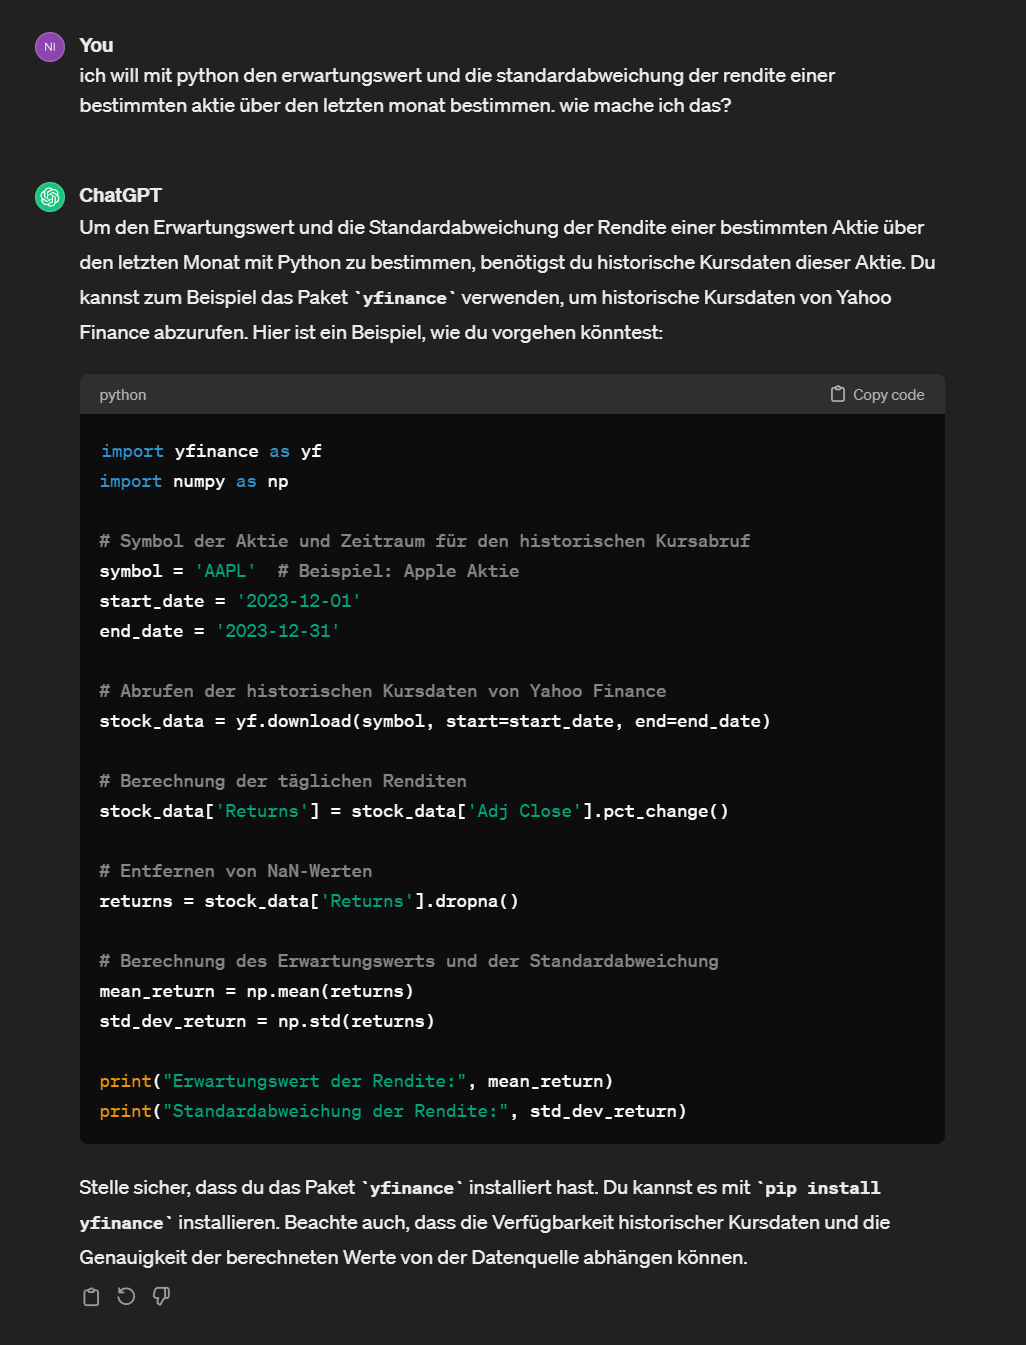
\includegraphics[width=0.6\linewidth]{images/chatgpt-answer-5.4.24.png}
    \caption{Screenshot der Konversation mit ChatGPT vom 5. April 2024}
    \label{fig:chatgpt-answer-5.4.24}
\end{figure}
\end{document}